\documentclass[12pt,oneside,final]{vlsithesis}
\title{Crawling and Analyzing Repository in GitHub}
\author{Zhongpei Zhang}
\degree{Master of Science}
\doctype{Thesis}
\dept{School of Computer Science}
\numberofmembers{3}

\membera{H. Wu}
\depta{Department of  Electrical and Computer Engineering}
\memberb{X. Yuan}
\deptb{School of Computer Science}
\memberc{J. Lu, Advisor}
\deptc{School of Computer Science}
%\memberd{D. Wu, Chair of Defense}
%\deptd{School of Computer Science}

\defenseyear{2016}
\defensedate{September 16, 2016}


\usepackage{amsmath}
\usepackage{graphicx}
\usepackage{caption}
\usepackage{subcaption}
%\usepackage[aboveskip=-5pt]{subcaption}
\usepackage{pbox}
\usepackage[ruled]{algorithm2e}
\usepackage{hyperref}
\usepackage{rotating}
\usepackage[numbers]{natbib}
\bibliographystyle{apalike}
\usepackage{appendix}
\usepackage{pgfplots}
\usepackage{comment}
\usepackage{array}
\usepackage{url}
\usepackage{booktabs}
\usepackage{multirow}
\usepackage{longtable}
%\usepackage{subfigure}
%\renewcommand{\thesubfigure}{(\Alph{subfigure})}
\captionsetup[subfigure]{skip=1pt}
\newcolumntype{P}[1]{>{\centering\arraybackslash}p{#1}}


\pgfdeclarelayer{background}
\pgfdeclarelayer{foreground}
\pgfsetlayers{background,main,foreground}

\usepackage{tikz}

\usetikzlibrary{shapes,snakes}
\usetikzlibrary{shadows}
\usetikzlibrary{positioning}
\usetikzlibrary{arrows}
\usetikzlibrary{calc} 



\newtheorem{Definition}{Definition}
\newtheorem{Example}{Example}
\newtheorem{Algorithm}{Algorithm}
\newtheorem{Theorem}{Theorem}
\newtheorem{Corollary}{Corollary}
\newtheorem{Lemma}{Lemma}
\newcommand{\mud}{\langle d \rangle}

\usepackage{CJK}
\newcommand{\Chinese}[1]{\begin{CJK}{UTF8}{gbsn}#1\end{CJK}}
\newcommand{\minitab}[2][l]{\begin{tabular}{#1}#2\end{tabular}}


%\date{}
%\linespread{1.3}

\begin{document}


\maketitle
\makeapproval
\pagenumbering{Roman}
\setcounter{page}{3}

\tikzstyle{user} = [circle, inner sep = 0pt, text centered, draw = black, fill=blue!30]
\tikzstyle{repository} = [rectangle, rounded corners, minimum width = 30 pt, minimum height = 15pt, text centered, draw = black,  fill=red!50]
\tikzstyle{language} = [ellipse, text centered, draw=black, minimum width=60pt, minimum height = 20pt, fill=orange!40]
\tikzstyle{hide} = [circle, inner sep = 1pt, draw = white]
\tikzstyle{node} = [circle, inner sep = 0pt, text centered, draw = black, fill=blue!30,  minimum size = 1cm]
\tikzstyle{arrow1} = [thick, ->, >=stealth]
\tikzstyle{arrow2} = [bend right, ->, thick]
\tikzstyle{arrow3} = [thick, ->, >=open triangle 45, line width = 1.5pt]
\tikzstyle{arrow4} = [thick, -]
\tikzset{every edge/.append style={font=\small}}
\tikzset{every node/.append style={font=\small}}

\makedeclaration

\abstract{
GitHub has become one of the most popular online software developing website. I have crawled the most popular software repositories (own over 500 star number) in GitHub, along with their contributors and stargazers. In total, we have crawled 10,665 repositories, 176,256 contributors, and 1,170,449 stargazers. One of the most important missions of analyzing is detecting communities from the network. While the heterogeneous Github network includes three objects, user, repository and programming languages and two kinds of relation between user and repository, i.e., star and contribute. Mining heterogeneous information network is a fresh and promising research field in data mining. A lot of algorithms has been proposed for heterogeneous network clustering. However, most of these methods directly cluster the heterogeneous networks. This thesis aims to transform the heterogeneous network to the homogeneous network using different schemes and then cluster the new network. We studied three weighting schemes, including dot product, Jaccard similarity and cosine similarity between the vector representations of objects. Then I cluster the homogeneous network by using modularity maximization optimization algorithms, in particular, greedy modularity maximization optimization algorithm and spectral modularity maximization optimization algorithm. The performance of clustering is evaluated using F-measure and rand index based on the programming language the software repository used. To compare the interaction between the weighting schemes and clustering algorithms, we applied out methods on GitHub dataset. Then we transformed the whole network to repository-repository and furthermore transformed it to the language-repository network. Based on this network, we discovered the relation between languages. Among 94 programming languages used by the top 10,000 projects, we studied their relations using several clustering methods. Overall, we find that languages fall into five communities, i.e., web and  scripting languages (JavaScrip, HTML, etc.), system programming languages (C, C++, etc.), OS X and IOS programming languages (Objective-C, Swift, etc.), numerical and statistical languages (Matlab, FORTRAN, Julia and R), and functional programming (Lisp, Scheme, etc.).}

%This thesis studies graph clustering algorithms, in particular, algorithms based on modularity maximization, and their applications on clustering software repositories in GitHub. I implemented four clustering algorithms, including the Garvin-Newman, greedy modularity maximization, spectral modularity optimization, and Laplacian algorithms, and compared their time complexity and accuracy on several datasets.  I crawled the most popular software repositories (own over 500 star number) in GitHub, along with their contributors and stargazers. In total, we have crawled 10,665 repositories,176,256 contributors and 1,170,449 stargzers. To find communities between repositories, this two-mode network is transformed into one-mode repository network with different weighting schemes. Weighting schemes are a variety of similarity measures between repositories. They include dot product, Jaccard similarity and cosine similarity between the vector representations of repositories. I will study the interaction between the weighting schemes and clustering algorithms. The performance of clustering is evaluated using F-measure and rand index based on the programming language the software repository used. }


%\dedication{}

\acknowledgements{
I would like to present my gratitude to my supervisor Dr. Jianguo Lu for his valuable assistance and support during the past two years.

I also would like to express my appreciation to Dr. Xiaobu Yuan, and Dr. Huapeng Wu. Thank you all for your valuable comments and suggestions to this thesis.

Finally, I want to thanks to my parents, my friends who give me consistent help over the past two years.
}
\tableofcontents
\listoftables
\listoffigures
%\listofappendix




\chapter{Introduction}
\pagenumbering{arabic}
\setcounter{page}{1}
Nowadays, GitHub\cite{1}, an open source website for software repositories, has become increasingly popular and attracts a great number of software developers around the world. It provides the services of code hosting, as some platforms have done before, such as SourceForge, BitBucket, and Aseembla. Different from these websites, it more focuses on the social features. Actually, GitHub could be seen as a storage of codes but also as a free and easy-to-use on-line tool for collaborative software development. Besides, it also offers a lot of functions to support the community of developers. The network of the users of GitHub can be regarded as a small-scale social network. In this network, the developer can follower those who attracts their attention. The GitHub provide a function called event, which may send an intermediate notification of the latest information about what happen to their following developers to the developer. Moreover, in GitHub, any user can create their own code repository. Every repository can be developed by more than one developer. The owner of the repository can add other collaborators and invite them to complete the repository together. But they are not the only one who can change the code of the repository. In fact, every developer who wants to join the development of the repository can make the contribution to it by forking. This action copies all the files of the repository to those who fork it, which allows the developers work independently without changing the original code. When the developers complete a new task, like fixing a bug, they can send pull requests to the owner of the original repository. Then the owner can review the changes that they have made and decide whether or not apply these changes in the original repository. Once the changes are accepted, the author becomes one collaborator of the original repository. The GitHub not only be used to develop software but also can be seen as a resource to search for high-quality software. The users can find out the repository which they are interested in and star and star it. Then when the software updates, they may get the latest information about it. The GitHub also provides download, clone in desktop and some other functions. For April 2016, GitHub claims that it has over 14 million users and over 35 million repositories, which makes it becoming the largest host of source code in the world. Therefore, mining data from GitHub and analyze these information has become an important study subject. 

%In the real world, most objects are not independent but often are instead connect to other objects, no matter the same type or other different types, in various methods. Datasets including interrelated objects are usually displayed as networks. There are two categories of the networks. One is homogeneous, which is only constructed by one type of objects and one kind of relationship between objects. For example, a social network only includes users and there is only one kind of relationship that one user follows another one. While, in reality, most of the networks are heterogeneous. A network includes multiple objects or different relationship between objects is a heterogeneous network\cite{philip2010link}. For instance, a citation network includes papers and authors. The author could collaborate  with other authors and one paper could be cited by other papers. So there are two kinds of objects and two categories of relationship. 

An important task in network data mining is clustering and it is also a classical object-related mission in network mining. Object clustering on networks, which is also known as community detection\cite{fortunato2010community} or group detection \cite{getoor2005link}, aims to distribute objects in a dataset to either separate or overlapping clusters\cite{han2011data} based on their relationship and similarity. Each cluster could also be call community\cite{newman2006modularity, girvan2002community}  or group \cite{getoor2005link}. (Note that the terms communities, cluster and group are same in this work.) Clustering has been widely studies for several years in various areas, such as machine learning, pattern recognition, and data mining. Unlike traditional attribute-based clustering techniques\cite{huang1998extensions, karypis1999chameleon,guha1998cure, zhang1996birch}, clustering based on the network structure also consider the links between objects. So clustering on the network is also called like-based clustering\cite{philip2010link} or relational clustering\cite{yin2006linkclus}. For homogeneous network clustering, we can directly apply the traditional clustering methods. While applying the traditional methods on the heterogeneous network usually leads to terrible results and this problem has drawn a lot of attention in recent years. One solution for this problems is directly clustering the heterogeneous network and simultaneously cluster objects of each type,  but this method is not available for a large network. Another one is heterogeneous-transformed homogeneous clustering \cite{huang2014clustering}, which means first transforming the heterogeneous network to homogeneous network and then clustering the homogeneous one. There has been a lot of researches about the directly clustering methods, but less attention has been paid on the heterogeneous-transformed homogeneous clustering. 

In my thesis, I cluster the programming languages and  investigate the relation between programming languages. Categorization of programming languages is an important approach to understanding languages. Languages can be clustered according to a variety of criteria, such as  by programming paradigms ( e.g., functional programming vs. OO programming), by genealogy (e.g., C is the ancestor of C++), by applications (e.g., numerical analysis vs. logic inferences), or by syntax similarities (e.g., Java vs. C\#).  Traditionally, categorizations are done based on anecdotal accounts, which are hard to verify and quantify. 

Thanks to the availability of open source projects such as GitHub, relations between languages can be derived from user interactions. GitHub lists the language for each project and the users who favour the project. Assuming that projects favoured by the same person are related in some way, the relationship between projects can be derived based on the common users they share. Based on the relations between projects, the language relation can be simply the sum of relations of repositories that use the language.  

Quantifying the relation is not a trivial task. Existing similarity metrics can not be applied directly. For instance, Jaccard similarity tends to biased towards popular repositories/languages--the more popular the repositories/languages are, the higher similarity they have.  To solve this problem, we represent each repository as a vector of users, and the similarity is the cosine of the vectors. Another problem is caused by very active users who give stars profusely to many projects.  Their weight should be reduced. Following the IDF(Inverse Document Frequency) heuristic in information retrieval, where popular words are discredited inversely proportional to their document frequencies, we also suggest reducing a user's weight inversely proportional to its stars he gives. 

Considering these two observations, we propose to use doc product-idf as the similarity function between two vectors of projects. To verify such weighting scheme, we evaluate it again others, including dot product, cosine, Jaccard Similarity, and cosine-idf.  We cluster projects using modularity maximization algorithm. The ground truth is labeled by languages: two projects belong to the same cluster is they are labeled by the same language.  Evaluating the result by F-measure and rand index, the experiment indicates that dot product-idf is the best weighting schemes.

We have applied the above method on the dataset we have crawled. For the data collection, I have crawled the whole list of GitHub users in May 2015. Then based on the user information, I collected the follower information and those repositories with at least 500 stars.  I also collect the contributor and stargazers of these repositories and create two networks, repository-contributor network, and repository-stargazer network. As the repository-stargazer network provides more information than the repository-contributor network, we used dot product-idf as the weighting scheme to reveal the relationship between communities of the repository-stargazer network. We separately detected 7 communities for greedy modularity algorithm and 4 communities for spectral modularity algorithm. From the result of both clustering algorithm, we found that there are some programming languages are usually belong to the same community, such web development programming languages (JavaScript, HTML, CSS and PHP), system programming languages (Python, C, C++ and Go) and programming languages for OS X and iOS system (Objective-C and Swift). 

We also investigated the relation between programming languages on three different clustering methods. These methods separately based on the high dimensional language-repository matrix, 2 dimensional language-repository matrix, and language-user matrix. From the experiment, it is difficult to decide which methods better performs the relation between programming languages, but we found some common phenomenon. Some pairs of programming languages are usually close, such as HTML\&CSS, C\&C++ and Matlab\&FORTRAN. The results can also have direct commercial applications. For instance, it can be applied in recommending programming related products, such as books, courses, jobs etc. When a programmer buys a Fortran book, she may be also interested in Matlab books. In addition, we find that languages fall into five communities, i.e., web and  scripting languages (JavaScrip, HTML, CSS, etc.), system programming languages (C, C++, Python, etc.), OS X and IOS programming languages (Objective-C, Swift, Objective-C++, etc.), numerical and statistical languages (Matlab, FORTRAN, Julia and R), and functional programming (List, Scheme, Racket, Haskell, etc.). 

Main contributions of the thesis can be summarized below: 
\begin{itemize}
\item We crawled a large network that contains millions of users and 10,000 top repositories. It is extremely time consuming to identify the top stared repositories. 
\item When transforming heterogeneous network to homogeneous network, we propose to use the IDF heuristics. The weighting scheme improves the clustering result significantly. 
\item We cluster programming languages using a variety of methods, including based on repositories, users and the reduced dimensionality of repositories. And our study surface some deeper knowledge between programming languages, such as FORTRAN and Matlab, Groovy and IDL are usually used in one repository. 
\end{itemize}

For software companies, the knowledge would help them to select the best combination of languages to support. For software developers, they can logically arrange the learn of programming languages. The results can also have direct commercial applications. For instance, it can be applied in recommending programming related products, such as books, courses, jobs etc. When a programmer buys a Fortran book, she may be also interested in Matlab books. 

The remainder of this thesis is structured as follows: In chapter \ref{chapter:relatedWork}, we introduce the previous works on heterogeneous network clustering and recent research on GitHub dataset. In chapter \ref{chapter:dataset}, we detailedly explain the process of crawling data from GitHub and describe the detail of our dataset. In chapter \ref{chapter:network transformation}, we present the three weighting schemes we used to transform the heterogeneous network to homogeneous network. Then in chapter \ref{chapter:Clustering Networks}, we introduce the two clustering methods based on the modularity maximization optimization strategy and evaluation measures. And we apply the methods on the subdatasets extracted from the dataset we collected. In chapter \ref{chapter:communities in repositories}, we applied the suitable weighting schemes on the whole network to find out the relation between repositories and then in chapter \ref{chapter:relationship between programming languages} we analyze the relation between programming languages. Finally, we summarize our work, give out the conclusions and describe the future work in chapter \ref{chapter:conclusion}.
%-------------------------------------------------------------------------------------
%\chapter{Review of the Literature}\label{chapter:relatedWork}
%In this chapter, we first review papers about  heterogeneous network clustering. Then we introduce recent research on GitHub datasets, such as the network structure and transparency and collaboration between users.  
%%-------------------------------------------------------------------------------------
%\section{Previous Work of Heterogeneous Network Clustering}
%\subsection{Mining Hidden Community in Heterogeneous Social Networks}
%\citet{cai2005mining} explore the question of mining hidden communities on heterogeneous social networks, which includes various categories of relationship. 
%
%\textbf{Method}
%As multiple, heterogeneous social networks are common in reality and they often affect the people's social activities together, \citet{cai2005mining} proposed a new approach for relation extraction and two algorithms for different situations. One is a regression-based algorithm. The algorithm finds a combination of relation to getting the tightest relationship between intra-community instances and the loosest relationship between the inter-community. But this approach may fail if the instances given by the user belong to only one community. 
%So to solve this problem they propose the mincut-based  algorithm, which considers the weakest connection in the extracted relation and use the value of minimum cut to evaluate the tightness of the graph.
%
%\textbf{Dataset}
%\citet{cai2005mining} used two datasets, one is the Iris dataset and another is DBLP dataset. The Iris dataset, which is widely utilized for evaluating clustering, contains 3 classes and each class represents a kind of Iris plant. Each class includes 50 instances, each of which has four features. For the DBLP dataset, it includes more than 500,000 articles and more than 1000 conferences(By May 2004). \citet{cai2005mining} took the authors as objects and treat the author publish the paper in the same conference as a category of the relation between authors to construct a network includes multiple relations between authors.
%
%\textbf{Experiment}
%For Iris dataset, the authors applied their regression-based relation extraction algorithm and  chosen the Normalized Cut algorithm to detective communities.  Then they compared the obtained label of each object with the ground truth. While for the DBLP dataset, the authors gave query example which belongs to the same community and they applied the MinCut based relation extraction algorithm to extract the hidden relation.
%
%\textbf{Result and Conclusion}
%The authors claimed that the experimental result on Iris and DBLP dataset implies that their algorithms improve the prediction accuracy compared with the baseline methods and it also convincingly finds valuable communities and relations. They also stated that the query-based relation extraction and community mining could be applied to a great number of new applications in social network analysis.
%%-------------------------------------------------------------------------------------
%\subsection{Co-clustering documents and words using bipartite spectral graph partitioning}
%\citet{dhillon2001co} treated the document collection as a bipartite graph between documents and words and used the spectral co-clustering algorithm to simultaneous cluster documents and words.
%
%\textbf{Methods}
%The authors proposed a bipartite spectral algorithm. First, for a given word-document network, create a $m \times n$ matrix A, where m is the number of document and n is the number of word. The value of each element $A_{ij}$ in A is equal to the weight between i and j. Suppose $D_{d}$ and $D_{w}$ separately is the degree matrix of document and word. Then form $A_{n} = D_{d}^{-1/2}AD_{w}^{-1/2}$. Next, calculate the second singular vectors v  and u of $A_{n}$.  Based on these two vectors, form the 1-dimensional data $ z = \left[
%\begin{matrix}
%D_{d}^{-1/2}u \\
%D_{w}^{-1/2}v
%\end{matrix}
%\right] $. At last, apply k-means algorithm on z to get the desired bipartition. The algorithm can also be applied to solve multipartition problem. We just need to compute $s = \lceil log_{2}c \rceil$ singular vectors U, V of $A_{n}$, where c is number of cluster you want to obtain. Then we form the l-dimensional matrix $ Z = \left[
%\begin{matrix}
%D_{d}^{-1/2}U \\
%D_{w}^{-1/2}V
%\end{matrix}
%\right] $ and run the k-means algorithm to get the c-way multipartition.
%
%\textbf{Dataset and Experiment}
%The authors mainly used two datasets to testify their algorithm. The first one the collections of Medline, Cranfield and Cisi. The there collections separately contain 1,033 medical abstracts, 1,400 aeronautical systems abstracts and 1460 information retrieval abstracts. To test the bipartition algorithm, they created mixtures including two of the three collections. While for testing multipartition algorithm, they mixed all three collections together. Besides, they also created the dataset consists 2340 Reuters news articles downloaded from Yahoo in October 1997\cite{boley1998hierarchical}. The articles can be divided into six categories: Entertainment(1,384), Health(494), Business(142), Spots(141), Politics(114) and Technology(114). The author extract two matrices form this collection, one includes 1459 and another contains 21839 words after deleting stop words.
%
%\textbf{Result and Conclusion}
%The valuable result proved that the bipartition algorithm performs good and the author also found that the top words in each cluster are those have the highest internal edge weight. The bipartition algorithm is able to recover the original clusters with removing the stop words. And  the multipartition algorithm also gives good results, no matter for the large or small dataset. The authors claimed that their algorithm using the singular vectors solve the real relaxation to the NP-complete graph bipartition question. 
%%-------------------------------------------------------------------------------------
%\subsection{Multi-way Clustering on Relation Graphs}
%\citet{banerjee2007multi} proposed a multi-way relation graph clustering(MRGC) to cluster objects of different communities simultaneously. This approach not only based on the intrinsic attribute values of entities but also the relationship between them.
%
%\textbf{Method}
%The authors introduced a multi-way clustering formulation extracted from the objective of capturing the maximal "information" in the original relation network. Based on the formulation and  minimum Bregman information(MBI) principle \cite{banerjee2007generalized}, the multi-way clustering algorithm considers each dimension in sequence. Then find the optimal clustering with respect to that dimension keeping everything else fixed and repeatedly compute the MBI solution. The process terminate until convergence. 
%
%\textbf{Dataset and Experiment}
%First, \citet{banerjee2007multi} tested their method on synthetic data to analyze the dependence of the clustering accuracy and the resulting approximation of the selection of Bergman divergence the multi-way clustering basis. Then the authors applied their approach on the subset, including 100 documents randomly selected from 4 newsgroups, of 20 Newsgroups data\cite{dhillon2003information}. To illustrate the utility of clustering on the relation graph structure, they created a subset consisting 100 movies and 39,031 users of the IMDB-EachMovie dataset\cite{banerjee2005model}. At last, for studying the collaborative filtering, the authors used a subset of MoiveLens dataset(movielens.umn.deu), which has 456 users, 600 movies and 19 movie-genre. 
%
%\textbf{Result and Conclusion}
%The authors claimed that their clustering techniques not only simultaneously  cluster multiple communities of objects but is also available for multiple relations network. They also suggested that the MRGC algorithm performs pretty good for handling high dimensional sparse dataset with mixed data categories. Besides, they stated their formulation can be extended to active, online and semi-supervised learning. 
%%-------------------------------------------------------------------------------------
%\section{Previous Work on GitHub Dataset}
%\subsection{Network Structure of Social Coding in GitHub}
%\citet{thung2013network} address the question what kind of the actual relationship between developers and projects in the social network of GitHub, a popular project hosting website, which provides a new experience to the developer cause they can easily share and connect with others. To understand the phenomenon of social coding better and analyze the features of the online social network of GitHub, the authors addresses four questions: Q1 "How strong are the relationship among projects?", Q2 "How strong are the relationship among developers?", Q3 "Which projects are the most influential?", Q4 "Which developers are the most influential?". 
%
%\textbf{Method}
%The authors introduce a method for constructing a sample network from GitHub. To create a project-project network, the authors first identify the developers for each project. They find all the projects that the developers have contributed to. There is a small set of projects and the authors figures whether  the input project is in the set. This method can also be used to construct the developer-developer network. Another algorithm described by the authors is the PageRank algorithm, which is introduced by\cite{brin1998anatomy}. This algorithm is designed for evaluating the importance of web pages. The authors use the equation below to calculate the PageRank value:
%\begin{align}
%	PR(p,i) = \dfrac{1- r}{T} + r\sum\limits_{q \in K_{p}} \dfrac{PR(q,i -1)}{\mid L_{q} \mid}
%\end{align}
%In this formula, r presents the probability of random transition, T is the total count of the web pages,  $ K_{p} $ is the set link to i, $ L_{q} $ is the set of an outbound link to page q.
%
%\textbf{Experiment}
%To answers the four proposed questions, the authors conducted four experiments. The experiment is based on 100,000 projects that obtained from GitHub API and randomly select 30,000 developers from the developers of the 100,000 projects. For the project-project relationship, the authors measured the count of edges in the graph. Then, they computed each node's degree, the number of inbound edges in this network. At last, the authors calculated the average shortest path between each pair of sample nodes and the diameter of the largest connected component. This method is also used in analyzing the developer-developer relationship. In addition, to identify the most influential project and developer, the authors ran the PageRank algorithm in both project-project and developer-developer networks and this algorithm returns the score for every project and developer, which could be used to order the projects and developers.
%
%\textbf{Result and Conclusion}
%Based on the evaluating results, the authors claim to observe that the degree distribution of projects follows a long tail distribution. Moreover, in the project-project network, the diameter of the largest connect component is 9 and the average shortest path is 3.7. Both of the numbers are lower than the results reported in other real networks \cite{leskovec2008planetary}, which means this project network is more interconnected than human social networks. On the other hand, the authors claim that the degree distribution does not appear the power law distribution in the developer-developer network. The value of the diameter of the largest connected component and the average shortest path are 5 and 2.47, separately. The authors claim that the low value implies that the social coding improves the collaboration among developers.The authors claim that the influential project is homebrew, which provides an easy-used package for Mac user to install UNIX tools, and this project owns 7233 developers. In addition, Joshua Peek, who the authors state is an influential developer, collaborate with other top influential developers on 81 projects.
%
%In this paper, the authors contribute to a great deal of  knowledge about social coding by analyzing the network of open source code website--GitHub. The authors claim that from the experiment the evaluation result displays that the degree distribution appears a power law phenomenon in the project-project network while does not follow a long tail distribution in the network of  developer-developer. In addition, according to the small value of the average shortest path in the largest graph of developers, the authors also claim that they have found that the social coding concept actually improves the collaboration among the developers.
%%-------------------------------------------------------------------------------------
%\subsection{Social Coding in GitHub: Transparency and Collaboration in an Open Software Repository}
%\citet{dabbish2012social} state that social web application enables users to follow and track a lot of others users activities. The transparency completely improves the collaboration and learning in complex online software development.The authors address two questions: 1) What inferences do people make when transparency is integrated into a web-based workspace? and 2) What is the value of transparency for collaboration in knowledge-based work?
%
%\textbf{Method}
%The authors propose a grounded method to analyze the transparency related inference in their interview answers. First, they labeled different types of inferences for examples in five interview transcripts. For this example, they identify the information made by GitHub system and the inferences made by participants based on the information. Then the authors compare these examples with the previously examined example and put the similar ones together. The process presents kinds of transparency related inferences and higher level behaviors supported by this inference. They repeat the process until the interviews no longer present new behaviors or categories. Based on the new idea, the authors state that they completed a series of semi-structured interviews with 24 GitHub users via email, phone or person by person. Based on the answers of interviews, the authors labeled the categories of inference and then tested what categories of higher-level activities supported by these inferences.
%
%\textbf{Result and Conclusion}
%Based on the evaluational experiments, the authors claim that transparency in GitHub allow developers to collaborate on a progress or a project more generally. In addition, the authors realize that the immediate prompt of what others are working on  or commenting helps developers find 'useful' and 'interesting' repositories and events. However, the authors also find out the transparency limits the communication between developers.
%
%The authors claim that they found four crucial elements of visible feedback drove a large number of inferences around commitment, work quality, community significance and personal relevance. The authors also claim that their findings inform the design of large-scale collaboration on social media and imply a serious of methods that transparency enable innovation, knowledge sharing and community construction.
%%-------------------------------------------------------------------------------------
%\subsection{Coding Together at Scale: GitHub as a Collaborative Social Network}
%\citet{lima2014coding} claim that the interaction happened on GitHub is the problem. GitHub has already become the most popular open source software platform and has over 3.5 million registered users and 10 million repositories in 2013. Interactions of GitHub users are complex and it happens in different ways. Investigating a different kind of interactions of developers could help us better understand the structure of open source software platform and the collaboration between the developers. 
%
%\textbf{Method}
%The authors propose a new idea constructing the social network. The authors derivate four networks from the dataset. The authors create a directed social graph  $ G_{F} $ describing the relationship between users and followers. The authors build a bipartite network $ G_{C} $ describing the repositories connected to the users' collaborations. The authors construct a bipartite network $ G_{S} $ representing  users assigning a star to the repository. The authors also describe the relationship between contributors and repositories by using a bipartite graph $ G_{N}$. 
%
%\textbf{Experiment}
%Based on the new idea, the authors conduct the experiment. The authors claimed that the experiment is based on a dataset including 183.54 million events, 2.19 million users information and  5.68 million repositories information. The authors analyzed the basic structure and calculate the distribution of contributors and watchers for each project and followers of each user. The authors also investigated the correlation between the social tie and repository. The authors studied the width and depth of the trees related to the forked repositories. The authors analyzed the relationship between the activity of users and the numbers of followers. The authors also research the geographic distributions of followers and collaborators.
%
%\textbf{Result and Conclusion}
%Based on the evaluational results, the authors state that the distribution of the numbers of collaborators each project, contributor of each project, stargazes of each project and the followers of user show a power-law shape. The authors also claim that the reciprocity of the social ties is very low. Besides, the authors claim that some very active users do not own a great number of followers. The authors also claim that the collaboration between developers usually happens on a small size project and a lot of collaborators prefer to work with other developers around a specific location.
%
%The authors claim that they analyze the events occurring on GitHub for 18 months from March 2012 to September 2013. The authors also claim that their work provides a new opinion about the complex collaboration on a large scale.
%
%-------------------------------------------------------------------------------------
\chapter{Review of the Literature}\label{chapter:relatedWork}
Association between programming languages has been studied using data from open sources such as SourceForge \cite{delorey2007programming}, GitHub \cite{sanatinia2016github} and StackOverflow \cite{vasilescu2013stackoverflow}. One approach is to use language co-occurrence in projects. Deloray et al. found that the closest pairs are (C, Perl), (C, C++), (Javascript, PhP). \citet{karus2011study} found associations such as (Java, XML). (C, make), (JavaScript, CSS) \cite{karus2011study}. Language co-occurrence can not reveal the similarity between languages.  Similar languages may not co-occur in a project.  Matlab and R are similar. In a project, either one of them is used, not both at the same time. The other approach is to use user interactions. \citet{vasilescu2013stackoverflow} use  StackOverflow data to study the similarities between language pairs based on user's language tags \cite{vasilescu2013stackoverflow}. \citet{sanatinia2016github} use user commit data in GitHub to study language relations. They focus on the top 10 languages and use k-means to cluster the programming languages. In this chapter, we will detail these related work. 
%-------------------------------------------------------------------------------------
\section{Programming Language Trends in Open Source Development:
An Evaluation Using Data from All Production Phase SourceForge Projects}
\citet{delorey2007programming} analyzed projects from SourceForge to realize the trends in programming language. 

\textbf{Dataset}
\citet{delorey2007programming} collected the CVS repositories Open Source projects hosted on Source Forge and data from SourceForge Research Archive(SFRA). They have totally crawled 9,997 projects and 23,83 authors. All these information are written in more than 7.5 million individual files and these files are distinctly changed over 25 million times. 

\textbf{Result and Conclusion}
For the popularity of programming language, \citet{delorey2007programming} found that web development languages becomes more popular, but the traditional desktop development languages are decreasing in popularity. Besides, although there is just a little of people like scripting languages, the number of these people remain consistent. The author also studied the use of multiple programming languages for individual projects and individual users. They claimed that only nearly tenth using three languages, less than a quarter using two languages and over two thirds using one language. At last, they believed that each year, the three most common languages profile were single language profiles. While for profiles written by two language, the most popular ones are web development profiles. 
%-------------------------------------------------------------------------------------
\section{On GitHub's Programming Languages}
\citet{sanatinia2016github} studied the popularity of programming languages and existence of trends in the relations between users, repositories, and programming languages on Github.

\textbf{Dataset}\citet{sanatinia2016github} designed  and implement a resilient distributed data collection system, which inlaces 200 collection advantage points to collect data from Github to avoid the limitation of Github API, that each hour can only sending 5000 requests. In total, the authors collected information of nearly 10 million (9,993,767) users and less than 17 million (16,812,452) repositories. For the user information, over 95\% are user account and the rest are organization account. For the repositories, they are designed by over 200 different programming languages, which is denoted by Github.                

\textbf{Method}
To identify the relationship between top 10 popular programming languages, \citet{sanatinia2016github} separately calculate the correlation between programming languages by the commits made by users and the repositories built by each users. Then utilizing the correlation as input, they clustered top 10 programming languages on Github by k-means clustering\cite{arthur2007k}.  Then the authors selected top 100 repositories of each top 10 programming languages and they created a directed graph to represent the relationship between the programming languages. In the graph, each vertex represents a programming language and the edge between each two vertices means whether these two programming languages are simultaneously used in one repository. Then they ran PageRank algorithm\cite{page1999pagerank} on the graph to rank the programming language. 

\textbf{Result and Conclusion}
From the collecting data, \citet{sanatinia2016github} claimed that JavaScript is the most popular programming language in Github, and it has more than 7 million stars, which is over twice that the second one. Through the experiment of top 10 programming languages, \citet{sanatinia2016github} discovered two clear communities. One is the "web programming" languages including JavaScript, PHP, Ruby and CSS. Another form for "System oriented programming" languages, such as C, C++ and Python. Based on the classification result, the authors created a phylogenetic tree for the use of programming languages Github. The authors also ranked top 1000 repositories using different metrics, i.e. percentage of lines of code and PageRank. They believed that HTML is utilized in many repositories with other programming languages, and it is followed by script languages, such as Perl and Makefile. 
%-------------------------------------------------------------------------------------
\section{StackOverflow and GitHub: Associations between software development and crowdsourced knowledge}
\citet{vasilescu2013stackoverflow} investigated the interaction between StackOverflow actions and the process of development, indicated by the change of code on Github. 

\textbf{Dataset}
\citet{vasilescu2013stackoverflow} downloaded the list of StackOverflow members and the history of their activities in August 2012. The information including 1,295,622 registered users from July 2008 to August 2012. All of this information are stored in XML format. On the other hand, the data of Github is collected from GHTorrent\cite{gousios2012ghtorrent} and the data is stored as MongoDB data dumps. This dataset contains 397,348 users and over 10 million (10,323,714) commits. Most of this information are crawled since July 2011 until April 2012. The authors merge these two datasets following a conservative method, if the computed MD5 hash of the Github user's email address is identical to the MD5 email hash of the StackOverflow user, to prevent the number of false positives. So they totally found 46,967 users who are active on both websites. 

\textbf{Experiment}
\citet{vasilescu2013stackoverflow} firstly took a macroscopic view to find how Github commits effect the actives on StackOverflow. The applied a "split-and-compare" method on the appropriate statistical testing process and compared multiple distributions. Then they took a intermediate view to understand the commit distribution of users. To satisfy this purpose, they improved their approach by defining a working rhythm. At last, they studied the interaction between activities on  Github and StackOverflow. 

\textbf{Result and Conclusion}
\citet{vasilescu2013stackoverflow} observed that people who commit a lot on Github prefer to answer questions rather than ask questions on StackOverflow. The also found that there is no connection between the working rhythm of Github contributors and their actives on StackOverflow.  In addition, they claimed that the active users on StackOverflow are also involved in a great number of contribution on Github  and they believed that StackOverflow improves commits on Github. 
%-------------------------------------------------------------------------------------
\section{A study of language usage evolution in open source software}
\citet{karus2011study} researched the evolution of combined use of programming languages on 22 open source software projects over 12 years. 

\textbf{Dataset}
\citet{karus2011study} created a dataset including 22 OSS projects and these projects are classified as two categories, desktop type and business(server) type. Projects, usually used in desktop environments, beyond to desktop type and those projects, providing business function, are regard as business type. For the files of these projects, 45 major file types are identified, such as C, C\#, C++. 

\textbf{Experiment}
\citet{karus2011study} extracted the user information to study their habits and discovered the combination of programming languages in projects. The mainly analyzed three major classes of developers, C/C++ developers, Java developers and XML developers. They also analyzed  the first commit made by developers to learn their initial experience. In addition, they studied the commits file types to find out which programming languages are used together and which file types are co-changed. 

\textbf{Result and Conclusion}
\citet{karus2011study} found that in the 22 OSS projects, the most popular programming language is XML, which is followed by Java and C. They also claimed that the files of the same type easily co-evolve, such as Java file most co-evolve with XML. They believed that XSL is important for the transformation of documents and creation of interfaces. While for developers, although most of them worked on more than programming languages during their studying period, new developers  just used a few number of programming languages on their first commit. Based on the usage of programming languages, the authors claimed that developers not only need to utilize multiple programming languages but also should understand different kinds of coding paradigms. 
%-------------------------------------------------------------------------------------
\chapter{Crawling GitHub}\label{chapter:dataset}
\section{GitHub}
GitHub is a web-based hosted service for Git repositories. Git is a popular open-source version control system. GitHub allows programmers to host remote Git repositories, and also adds a wealth of community-based services. It is a social networking site for programmers. Users can follow others to know their recent activities, and invite other users to collaborate on one repository. 
\begin{figure*}
	\centering
	\begin{tikzpicture}
	\node(l1) at (3, 5)[language]{L1};
	\node(l2) at (9, 5)[language]{L2};
	\node(r1) at (1, 3)[repository]{R1};
	\node(r2) at (4.25, 3)[repository]{R2};
	\node(r3) at (7.75, 3)[repository]{R3};
	\node(r4) at (11, 3)[repository]{R4};
	\node(u1) at (0,0)[user]{U1};
	\node(u2) at (2,0)[user]{U2};
	\node(u3) at (4,0)[user]{U3};
	\node(u4) at (6,0)[user]{U4};
	\node(u5) at (8,0)[user]{U5};
	\node(u6) at (10,0)[user]{U6};
	\node(u7) at (12,0)[user]{U7};
	\draw [arrow1] (r1) --(l1);
	\draw [arrow1] (r2) --(l1);
	\draw [arrow1] (r2) --(l2);
	\draw [arrow1] (r3) --(l2);
	\draw [arrow1] (r4) --(l1);
	\draw [arrow1] (r4) --(l2);
	\draw [arrow1] (u1) --(r1);
	\draw [arrow1] (u1) --(r2);
	\draw [arrow1] (u2) --(r1);
	\draw [arrow1] (u2) --(r3);
	\draw [arrow1] (u3) --(r1);
	\draw [arrow1] (u3) --(r4);
	\draw [arrow1] (u4) --(r2);
	\draw [arrow1] (u4) --(r3);
	\draw [arrow1] (u5) --(r2);
	\draw [arrow1] (u6) --(r3);
	\draw [arrow1] (u6) --(r4);
	\draw [arrow1] (u7) --(r1);
	\draw [arrow1] (u7) --(r3);
	\draw [arrow1] (u7) --(r4);
	\draw [arrow2] (u1) to node [auto] {} (u3);
	\draw [arrow2] (u2) to node [auto] {} (u5);
	\draw [arrow2] (u3) to node [auto] {} (u4);
	\draw [arrow2] (u3) to node [auto] {} (u7);
	\draw [arrow2] (u4) to node [auto] {} (u7);
	\draw [arrow2] (u5) to node [auto] {} (u2);
	\end{tikzpicture}
	\caption{GitHub network structure}
	\label{fig:GitHub network}
\end{figure*}
GitHub has two kinds of objects, i.e., users and repositories.  Figure \ref{fig:GitHub network} illustrates their relationships. Each repository is labeled by programming languages, so we also add programming languages in this graph. In this figure, we can notice that there are three different kinds of relationships:

\begin{itemize}
	\item Users to Users: A user follows other users. 
	\item User to Repository:
	\begin{itemize}
		\item A user contributes to a repository: A user participates in the development  of a repository. The contribution includes adding codes, deleting codes and send commits. %Those users who contribute to one repository could be called the contributors to the repository. 
		\item A user stars a repository: A user can star a repository. Those users who star a  repository are called the stargazers of the repository. 
	\end{itemize}

	\item Repositories to Programming Languages: Repositories are labeled by programming languages based on the number of lines of code. As some repositories are written by using different programming languages, one repository could be labeled by more than one programming language. 
\end{itemize}

To analyze GitHub, we first crawl these three kinds of objects. The crawling process and the obtained networks are described in the next subsections. 

\section{User Network}

In the User network, the nodes are the users. There is a link from one node to another if one user follows the other. We crawled all the users and the relationships. The crawling is a challenging task due to the access restriction imposed by GitHub. Each hour an account can send maximal 5000 requests. Each request can return certain data, such as getting the basic information of a user, or a list of its followers. But the list is restricted as well-- each request will return one page that contains at most 30 followers. To obtain more followers, additional requests need to be sent to flip through the pages. Because of the limitation on the number of requests and the length of the return list, it is not easy to collect all the data.  

More specially,  we use the API provided by GitHub to collect the data. %GitHub API is a powerful and convenient tool to crawl data from GitHub. 
First, we need to require authentication by GitHub API and there are three methods to authenticate through GitHub API. The easiest way to authenticate with the GitHub API is by simply utilizing your GitHub login and password via basic authentication.  Then we send requests to GitHub API to collect the information we are interested in. All data is sent and received in JSON format.

\subsection{Crawling details}
For the user network, we collected all the users and their followers. The crawling process is described below.
\begin{itemize}
	\item Users: As user id is numbered sequentially\cite{2}, we repeatedly send request  "https://api.GitHub.com/users?since= \textbf{id};rel='next'"to the service to obtain all the users. In the request, 'since' represents the integer id of the last user you have collected and "rel = 'next'" means getting the next user. For instance, if we let id equals to 136, after sending a request, we receive the information of the user whose id is 137. 
	
Although the IDs are numbered sequentially, some users were deleted, resulting null return. In this case,  we increment the ID until the next user is found. The process of crawling terminates until there is no user returned by the API services. 

Each hour the service returns maximal 5000 different users as the limitation of GitHub API. The information of each user contains login,  id and a serious of URLs for its followers, repositories etc.. Figure \ref{fig:user information} is an example of the user information we collected from GitHub API.
	\begin{figure*}
		\centering
		\includegraphics[width = 5in]{figure/user_information}
		\caption{Example of user information}
		\label{fig:user information}
	\end{figure*}  
	\item Followers: Using the login (the username provided for register) of each user,  we repeatedly sent request  "https://api.GitHub.com/users/\textbf{user login} /followers?page=\textbf{page number}" to the API. Each request returns one page of its followers and each page contains 30 followers. To retrieve all the followers, we flip through the pages until the service returns an empty without any followers information. 
\end{itemize}

\subsection{Crawled data}
The crawling was done from May 2015 to July 2015. The data of users and followers we collected is summarized in Table \ref{tab:user and follower dataset}:
\begin{table*}[h]
	\centering
	\begin{tabular}{c|c} \toprule
		Item & Number \\ \hline
		Users & 12,007,048 \\ 
		Users have followers & 1,190,388 \\ 
		Followers & 1,175,466 \\ 
		Relationship between user and followers & 6,986,128 \\ \bottomrule
	\end{tabular}
	\caption{User and follower dataset}
	\label{tab:user and follower dataset}
\end{table*}

Note that in the user graph, the vast majority (90\%) of the vertices (users) are isolated, do not connect with any other nodes by the following relationship.  For all users, the average number of followers is only 0.58. After removing isolated nodes, the graph only contains 1,668,324 vertices and 6, 986,128 edges. The average degree of followers rises to 4.19. Fig \ref{fig:degree distribution of followers} plots the degree distributions of the graph and we noticed that the user degree distribution is close to the power law degree distribution, which is similar to other networks, such as Twitter \cite{kwak2010twitter} and Facebook \cite{ugander2011anatomy}. While, for Twitter, the average number of followers is 208 and the number of Facebook is 155.
\begin{figure*}
	\centering
	\includegraphics[width = 2.8 in]{figure/user_degree.eps}
	\caption{Degree distribution of followers}
	\label{fig:degree distribution of followers}
\end{figure*} 

\section{Repository-User Network}

There are two types of repository-user networks, each is a bipartite graph. One is the repository-stargazer graph, another is the repository-contributor graph. In the repository-stargazer graph, there are two types of nodes, i.e., repositories and users. There is an edge between a repository and a user if the user gives a star or contribution to the repository. The user is also called a stargazer or contributor.

\subsection{Crawling details}
\begin{itemize}
	\item Repository: We scan repositories associated with each user. This is enabled by an HTTP request like "https://api.GitHub.com/users/\textbf{user login}/repos?page=\\\textbf{page number}". As the large number of users, there are over 35 millions of repositories but not all of them are useful for us. We just scanned the repository list of each user and downloaded the information of those repositories whose star count is over 500. Because one repository has over 500 stars means this repository is popular and a great number of users follow this repository, these popular repositories can present the features of the whole network in some degree. Figure \ref{fig:repository information} is an example of the repository. Each repository contains id, language, which is labeled by GitHub based on the total size of the files that belongs to each programming language, and several links to its attributes, such as its languages, contributors, and stargazers. To obtain details of the language, contributors or stargazers, we need to send requests again.
	\begin{figure*}
		\centering
		\includegraphics[width = 3.6 in]{figure/repository_information}
		\caption{Example of repository information}
		\label{fig:repository information}
	\end{figure*}
	\item Stargazers: As we have the name of repositories, we could collect the stargazers information of repositories. We sent request "https://api.GitHub.com/repos/\\\textbf{repository name}/stargazers?\textbf{page number}" to the service and then received the information of stargazers of repositories. And we also used the page number to guarantee that all the stargazers of the repository have been collected. 
	\item Contributors: Same as the crawling of contributors information, we sent request "https://api.GitHub.com/repos/\textbf{repository name}/contributors?\textbf{page number}" to the service and then received the information of contributors of repositories. As each page only contents 30 contributors, we added the page number to promise all of these contributors information have been crawled.
	\item Programming Languages: For the repository, we have already collected the programming language of repository labeled by GitHub. While, some repositories may use more than one kind of program language. To get all the programming languages that the repository used, we sent request " https://api.GitHub.com\\/repos/\textbf{repository name}/languages" to API and download all the information including the list of programming languages and the number of lines of code for each programming language. Figure \ref{fig:language information} is an example. This repository is written by two programming languages, C and Python. There are 78,769 lines of code is written by C and 7,769 is written by Python in this repository.
	\begin{figure*}
		\centering
		\includegraphics[width = 5 in]{figure/language_information}
		\caption{Example of language information}
		\label{fig:language information}
	\end{figure*}
\end{itemize}

\subsection{Crawled data}
The repository and user data are summarized in Table \ref{tab:repository and user dataset}.  From the table, we can see that the number of stargazers is over 6 times than the number of contributors. Furthermore, the connection between repository and stargazer is over 50 times than the connection between repository and contributor. 
For the repository-stargazer network, a user gives 15.73 stars in average, and a repository receives 1,726.07 stars in average. Figure \ref{fig:degree distribution of repository-stargazer} shows the distributions of the in-degrees of repositories (a) and  out-degrees of the stargazers (b). The in-degree of repositories is the number of stargazers of repositories and the out-degree of stargazers is the number of repositories that users star. From the figures,  we realized that the out-degree distribution of stargazers displays the power law distribution. Actually, the in-degree of repositories should also show this, but as we just selected the repository with over 500 stars, we just plotted part of the in-degree distribution of all repositories.
\begin{table*}
	\centering
	\begin{tabular}{c|c} \toprule
		Item & Number \\ \hline
		Repositories & 10,665 \\ 
		Stargazers &  1,170,449 \\ 
		Contributors & 176,256 \\ 
		Relationship between repositories and stargazers & 18,408,518 \\ 
		Relationship between repositories and contributors & 354,870 \\ 
		Different programming languages used for these repositories & 94 \\ \bottomrule
	\end{tabular}
	\caption{Repository and user dataset}
	\label{tab:repository and user dataset}
\end{table*}

% \begin{figure*}
%    	\centering
%  	\subfigure[In-degree distribution of repository]{
%  		\includegraphics[width=2.8in]{figure/pindegree_star.eps}}
%  	\subfigure[Out-degree distribution of stargazers]{
%  		\includegraphics[width=2.8in]{figure/uoutdegree_star.eps}}
%  	\caption{Degree distribution of repository-stargazer network}
%  	\label{fig:degree distribution of repository-stargazer}
%  \end{figure*}

\begin{figure*}
	\centering
	\subcaptionbox{In-degree distribution of repository}{
		\includegraphics[width = 2.8 in]{figure/pindegree_star.eps}}
	\subcaptionbox{Out-degree distribution of stargazers}{
		\includegraphics[width = 2.8 in]{figure/uoutdegree_star.eps}}
	\caption{Degree distribution of repository-stargazer network}
	\label{fig:degree distribution of repository-stargazer}
\end{figure*}

\begin{figure*}
	\centering
	\subcaptionbox{In-degree distribution of repository}{
		\includegraphics[width = 2.8 in]{figure/pindegree_con.eps}}
	\subcaptionbox{Out-degree distribution of contributors}{
		\includegraphics[width = 2.8 in]{figure/uoutdegree_con.eps}}
	\caption{Degree distribution of repository-contributor network}
	\label{fig:degree distribution of repository-contributor}
\end{figure*}

%From the data, we noticed that the number of stargazers is far more than the number of contributors. For the repository-stargazer network, the average in-degree of repository is 1,726.07 and the average out-degree of stargazer is 15.73. Figure \ref{fig:degree distribution of repository-stargazer} a and b separately displays the in-degree distribution of repository and the out-degree distribution of stargzaers. While, for the repository-contributor network, the average in-degree of repository is 33.27 and the average out-degree of contributors is 2.01. Figure \ref{fig:degree distribution of repository-contributor} a and b separately describes the in-degree distribution of repository and the out-degree distribution of contributors. For the programming languages, we totally collected 95 different ones and Table \ref{tab:programming languages} displays the number of repositories for each programming languages. From the table, we can see that the number of JavaScript repository, which is 2258,  is far more than the number of repository labeled by other programming languages. And only 34 programming languages have more than ten repositories. Most of programming languages just have less than ten repository and 34 programming languages only have one repository. We also noticed that those programming languages has a great number of repository are also popular used in real life. So by analyzing the data we have collected, the result may also reflect the relationship between programming languages in real world.

The repository-contributor network is much more sparse. The average in-degree of the repository is 33.27, and the average out-degree of the contributor is 2.01. Here, the in-degree of repositories is the number of contributors of one repository and the out-degree of a contributor is the number of repositories that the user participates in.  Figure \ref{fig:degree distribution of repository-contributor} (a) and (b) separately describes the in-degree distribution of repositories and the out-degree distribution of contributors. From the figure, we noticed that both degree distribution follow the power law distribution.

Among these 10,665 repositories, there are 94 different programming languages used. Table \ref{tab:programming languages} shows the number of repositories for each programming language. From the table, we can see that the JavaScript is the most popular language (2258), followed by Java (960) and Objective-C (932). Besides, only 34 programming languages have more than ten repositories and there are 487 repositories are unlabelled. 
\begin{table*}
	\renewcommand\arraystretch{0.65}
	\small \centering
	\begin{tabular}{rr|rr} \toprule
		Programming language & Number of repository & Programming language & Number of repository \\ \hline
		JavaScript&2866&Objective-C++&3 \\  
		Java&959&Arduino&3 \\  
		Objective-C&932&Nginx&3 \\  
		Python&909&Matlab&3 \\  
		Ruby&883&D&3 \\  
		Unlabelled&487&PostScript&2 \\  
		PHP&461&Perl6&2 \\  
		C&395&Scheme&2 \\  
		HTML&356&Batchfile&2 \\  
		Go&356&F\#&2 \\  
		CSS&318&Vala&2 \\  
		C++&310&Pascal&2 \\  
		Swift&234&XML&1 \\  
		Shell&212&IDL&1 \\  
		C\#&169&MoonScript&1 \\  
		VimL&128&wisp&1 \\  
		CoffeeScript&111&Modelica&1 \\  
		Clojure&78&Yacc&1 \\  
		Scala&70&NSIS&1 \\  
		Emacs Lisp&38&PLpgSQL&1 \\  
		Perl&33&Racket&1 \\  
		Lua&29&AGS Script&1 \\  
		Haskell&28&SQLPL&1 \\  
		Erlang&27&Mirah&1 \\  
		TeX&23&Awk&1 \\  
		Rust&22&GLSL&1 \\  
		Makefile&19&FORTRAN&1 \\  
		Jupyter Notebook&15&Mathematica&1 \\  
		TypeScript&14&Nix&1 \\  
		Groovy&12&PigLatin&1 \\  
		ActionScript&11&Protocol Buffer&1 \\  
		R&11&Vue&1 \\  
		OCaml&11&Nimrod&1 \\  
		Assembly&10&CMake&1 \\  
		Elixir&8&Crystal&1 \\  
		PowerShell&7&KiCad&1 \\  
		Groff&5&PureBasic&1 \\  
		Haxe&5&Cuda&1 \\  
		ApacheConf&5&Frege&1 \\  
		XSLT&4&nesC&1 \\  
		Processing&4&Stan&1 \\  
		Julia&4&Elm&1 \\  
		Objective-J&4&Arc&1 \\  
		Kotlin&4&Handlebars&1 \\  
		Common Lisp&4&Red&1 \\  
		LiveScript&4&QML&1 \\  
		Eagle&4&Puppet&1 \\ \bottomrule
	\end{tabular}
	\caption{Programming Languages}
	\label{tab:programming languages}
\end{table*}

%-------------------------------------------------------------------------------------
\subsection{Sub Networks}\label{section:sub networks}
In my experiments, we extracted four subnetworks, Python\&HTML, Objective-C\&C, PHP\&CSS, and Java\&Ruby, from the repository-stargazer network and repository-contributornetwork. The details of the subnetworks are shown in Table \ref{tab:detail of datasets}. From the table, we noticed that except Java\&Ruby dataset, all the other three datasets are unbalanced dataset and Java\&Ruby dataset is the largest one, totally  including 1842 repositories, 41,034 contributors, and 427,205 stargazers. On the contrary, PHP\&CSS dataset is the smallest one with only 779 repositories. We also found that although the repository of PHP\&CSS network is much less than Objective-C\&C network, PHP\&CSS has more contributors than Objective-C\&C and the number of stargazers is almost equal. Besides, for the average degree of contributors of four datasets, it is no more than 2. But the average degree of stargazer is at least almost 3 times of the average degree of contributor, which means the repository-stargazer network provides more information and it could obtain better clustering results. 
\begin{table*}
	\centering
	\begin{tabular}{c|cccc}\toprule
		Dataset & Python and HTML & Objective-C and C & PHP and CSS & Java and Ruby \\ \hline
		\multirow{2}{*}{Repository} & 909 Python& 932 Objective-C& 461 PHP & 959 Java \\ 
		& 356 HTML & 395 C & 318 CSS& 883 Ruby\\
		Contributor &  35,987 & 20,893 & 24,100 & 41,034 \\
		Stargazer & 453,451 &  332,846 & 326,300 & 427,205 \\
		r-c relation&  50,381 & 29,677 & 34,104 & 68,916 \\
		r-s relation &  2,115,079 &  2,019,679 & 1,294,113 & 2,841,085 \\ 
		av degree-c &  1.40 &  1.42 & 1.41 & 1.68 \\
		av degree-s &  4.66 &  6.07 & 3.97 & 6.65 \\ \bottomrule
	\end{tabular}
	\caption{Detail of Datasets, r-c relation means relation between repository and contributor, r-s relation means relation between repository and stargazer, av degree-c means average degree of contributors, av degree-s means average degree of stargazers}
	\label{tab:detail of datasets}
\end{table*}
%-------------------------------------------------------------------------------------
\chapter{Network Transformation}\label{chapter:network transformation}
To cluster the repositories, I applied the heterogeneous-transform homogeneous network clustering \cite{huang2014clustering} on the GitHub dataset that we have crawled. First, I transformed the heterogeneous network constructed by the repositories and users to a homogeneous network which only includes repositories. For the process of transformation, we selected three kinds of weighting schemes, dot product, cosine similarity and Jaccard similarity to represent the similarity between repositories. 

We transformed the repository-user networks to repository networks using three weighting schemes, dot product, cosine similarity and Jaccard similarity. In addition, to reduce the effect of users that participate in a large number of repositories, we also applied the inverse document frequency on the repository-user subnetworks and then transformed the new heterogeneous network to the homogeneous one. As Jaccard similarity is only available for the binary object, we just utilized dot product and cosine similarity to complete the transformation. 


Based on the relationship between repositories and users(contributors or stargazers), we can construct the repository-user network, a heterogeneous network that includes different kinds of vertices. As the modularity optimization algorithm is only applied to the homogeneous network, which only includes one kind of vertex, we should transform the heterogeneous network into a homogeneous one, which means we should remove the user vertex and form a network only includes repositories(as Figure \ref{fig:hetro_to_homo} shown). To satisfy this purpose, we need to determine the similarity between two repositories. In order to represent the similarity, we need to calculate the similarity score between two repositories.  For the transformation, we select three different categories of weighting schemes, dot product, cosine similarity and Jaccard similarity. In addition, the repository-user network can also be shown as a matrix. For example, the repository-user network shown in Figure \ref{fig:hetro_to_homo} (a) can be represented by the matrix shown in Table \ref{tab:repository-user matrix}. Therefore, we can consider each repository as a vector whose element represent the relationship between users and the repositories. If the user is connected to the repository, the value of the element is 1, otherwise is 0. Here we give the definition of the three similarity scores.  
\begin{figure*}
	\centering
	\subcaptionbox{Repository-user network}{
		\begin{minipage}[b]{0.45\textwidth}
			\centering
			\resizebox{2in}{!}{
				\begin{tikzpicture}
				\node(r1) at (0, 4)[repository]{R1};
				\node(r2) at (4, 4)[repository]{R2};
				\node(r3) at (4, 0)[repository]{R3};
				\node(r4) at (0, 0)[repository]{R4};
				\node(u1) at (2,4)[user]{U1};
				\node(u2) at (3,2)[user]{U2};
				\node(u3) at (0,2)[user]{U3};
				\node(u4) at (4,2)[user]{U4};
				\node(u5) at (2,2)[user]{U5};
				\node(u6) at (2,0)[user]{U6};
				\node(u7) at (1,2)[user]{U7};			
				\draw [arrow4] (u1) --(r1);
				\draw [arrow4] (u1) --(r2);
				\draw [arrow4] (u2) --(r2);
				\draw [arrow4] (u2) --(r3);
				\draw [arrow4] (u3) --(r1);
				\draw [arrow4] (u3) --(r4);
				\draw [arrow4] (u4) --(r2);
				\draw [arrow4] (u4) --(r3);
				\draw [arrow4] (u5) --(r2);
				\draw [arrow4] (u6) --(r3);
				\draw [arrow4] (u6) --(r4);
				\draw [arrow4] (u7) --(r1);
				\draw [arrow4] (u7) --(r2);
				\draw [arrow4] (u7) --(r3);
				\draw [arrow4] (u7) --(r4);
				\end{tikzpicture}}
		\end{minipage}}
		\begin{minipage}{0.1\textwidth}
			\begin{tikzpicture}
			\node(h1) at (-1,5)[hide]{}; 
			\node(h2) at (1,5)[hide]{};
			\node(h3) at (0,0)[hide]{};
			\draw[arrow3] (h1) -- (h2);
			\end{tikzpicture}
		\end{minipage}
	\subcaptionbox{Repository-repository network}{
		\begin{minipage}[b]{0.4\textwidth}
			\centering
			\resizebox{2in}{!}{
				\begin{tikzpicture}
				\node(r1) at (0,4)[repository]{R1};
				\node(r2) at (4,4)[repository]{R2};
				\node(r3) at (4,0)[repository]{R3};
				\node(r4) at (0,0)[repository]{R4};
				\draw [arrow4](r1) -- (r2);
				\draw [arrow4](r1) -- (r3);
				\draw [arrow4](r1) -- (r4);
				\draw [arrow4](r2) -- (r3);
				\draw [arrow4](r2) -- (r4);
				\draw [arrow4](r3) -- (r4);
				\end{tikzpicture}}
		\end{minipage}}	
	\caption{Heterogeneous network transform to homogeneous network}
	\label{fig:hetro_to_homo}
\end{figure*}

\begin{table*}
	\centering
	\begin{tabular}{c|ccccccc} \toprule
		& U1 & U2 & U3 & U4 & U5 & U6 & U7\\ \hline
		R1 & 1 & 0 & 1 & 0& 0& 0& 1\\ 
		R2 & 1 & 1 & 0 & 1& 1& 0& 1\\ 
		R3 & 0 & 1 & 0 & 1& 0& 1& 1\\ 
		R4 & 0 & 0 & 1 & 0& 0& 1& 1\\ \bottomrule
	\end{tabular}
	\captionof{table}{Repository-user matrix}
	\label{tab:repository-user matrix}
\end{table*}
%-------------------------------------------------------------------------------------
\section{Dot Product}
For a repository-user network, the dot product\cite{strang2011introduction} of two repositories is the number of shared users(stargazers or contributors) between these two repositories. Here is the definition of dot product. For two vectors $ A = [A_{1}, A_{2}, \dots A_{n}]$  and $ B = [B_{1}, B_{2}, \dots B_{n}]$, the dot product is
\begin{equation*}
Dot Product(A,B) = A \cdot B = A_{1}B_{1} + A_{2}B_{2} + \dots + A_{n}B_{n}
\end{equation*}
%dot product of A and B
Here we give an example to explain(see Figure \ref{fig:network transformation} (a) and (b)) how to using the dot product to transform the repository-user network to repository-repository network. If we want to calculate the dot product between R1 and R4, we notice that R1 = [1, 1, 1, 0, 0, 0, 1] and R4 = [0, 0, 1, 0, 0, 1, 1], so the dot product of R1 and R4 is the dot product of these two vectors, then 
\begin{equation*}
Dot Product(R1,R4) = R1 \cdot R4 = 0 + 0 + 1 + 0 + 0 + 0 + 1 =2
\end{equation*}
In Figure \ref{fig:network transformation}, (a) and (b) displays the dot product transformation for the network and in Table \ref{tab:matrix transformation} (a) and (b) displays the dot product transformation of the matrix.

%\begin{table*}
%	\centering
%	\begin{tabular}{cc}\\
%		\subcaptionbox{Repository-user network}{
%		\begin{minipage}{0.45\textwidth}
%			\centering
%			\resizebox{3.1in}{!}{
%				\begin{tikzpicture}
%				\node(r1) at (0, 6)[repository]{R1};
%				\node(r2) at (6, 6)[repository]{R2};
%				\node(r3) at (6, 0)[repository]{R3};
%				\node(r4) at (0, 0)[repository]{R4};
%				\node(u1) at (3,6)[user]{U1};
%				\node(u2) at (4,3)[user]{U2};
%				\node(u3) at (0,3)[user]{U3};
%				\node(u4) at (6,3)[user]{U4};
%				\node(u5) at (8,3)[user]{U5};
%				\node(u6) at (3,0)[user]{U6};
%				\node(u7) at (2,3)[user]{U7};
%				\node(hide) at (-3,3)[hide]{};
%				\draw [arrow4] (u1) --(r1);
%				\draw [arrow4] (u1) --(r2);
%				\draw [arrow4] (u2) --(r2);
%				\draw [arrow4] (u2) --(r3);
%				\draw [arrow4] (u3) --(r1);
%				\draw [arrow4] (u3) --(r4);
%				\draw [arrow4] (u4) --(r2);
%				\draw [arrow4] (u4) --(r3);
%				\draw [arrow4] (u5) --(r2);
%				\draw [arrow4] (u6) --(r3);
%				\draw [arrow4] (u6) --(r4);
%				\draw [arrow4] (u7) --(r1);
%				\draw [arrow4] (u7) --(r2);
%				\draw [arrow4] (u7) --(r3);
%				\draw [arrow4] (u7) --(r4);
%				\end{tikzpicture}}
%		\end{minipage}}&
%	\subcaptionbox{Dop product transformation}{
%		\begin{minipage}{0.45\textwidth}
%			\centering
%			\resizebox{2in}{!}{
%				\begin{tikzpicture}
%				\node(r1) at (0,6)[repository]{R1};
%				\node(r2) at (6,6)[repository]{R2};
%				\node(r3) at (6,0)[repository]{R3};
%				\node(r4) at (0,0)[repository]{R4};
%				\draw [arrow4](r1) --node[above, sloped]{2} (r2);
%				\draw [arrow4](r1) --node[right, pos = 0.3]{1} (r3);
%				\draw [arrow4](r1) --node[left, pos = 0.65]{2} (r4);
%				\draw [arrow4](r2) --node[pos = 0.65, right]{3} (r3);
%				\draw [arrow4](r2) --node[pos = 0.75, right]{1} (r4);
%				\draw [arrow4](r3) --node[below, sloped]{2} (r4);
%				\end{tikzpicture}}
%		\end{minipage}}	\\
%	\subcaptionbox{Cosine similarity transformation}{
%		\begin{minipage}{0.45\textwidth}
%			\centering
%			\resizebox{2in}{!}{
%				\begin{tikzpicture}
%				\node(r1) at (0,6)[repository]{R1};
%				\node(r2) at (6,6)[repository]{R2};
%				\node(r3) at (6,0)[repository]{R3};
%				\node(r4) at (0,0)[repository]{R4};
%				\draw [arrow4](r1) --node[above, sloped]{$2\sqrt{15}/15$} (r2);
%				\draw [arrow4](r1) --node[right, pos = 0.3]{$\sqrt{3}/6$} (r3);
%				\draw [arrow4](r1) --node[left, pos = 0.65]{$2/3$} (r4);
%				\draw [arrow4](r2) --node[pos = 0.65, right]{$3\sqrt{5}/10$} (r3);
%				\draw [arrow4](r2) --node[pos = 0.85, right]{$\sqrt{15}/15$} (r4);
%				\draw [arrow4](r3) --node[below, sloped]{$\sqrt{3}/3$} (r4);
%				\end{tikzpicture}}
%		\end{minipage}}	&
%	\subcaptionbox{Jaccard similarity transformation}{
%		\begin{minipage}{0.45\textwidth}
%			\centering
%			\resizebox{1.8in}{!}{
%				\begin{tikzpicture}
%				\node(r1) at (0,6)[repository]{R1};
%				\node(r2) at (6,6)[repository]{R2};
%				\node(r3) at (6,0)[repository]{R3};
%				\node(r4) at (0,0)[repository]{R4};
%				\draw [arrow4](r1) --node[above, sloped]{1/3} (r2);
%				\draw [arrow4](r1) --node[right, pos = 0.3]{1/6} (r3);
%				\draw [arrow4](r1) --node[left, pos = 0.65]{1/2} (r4);
%				\draw [arrow4](r2) --node[pos = 0.65, right]{1/2} (r3);
%				\draw [arrow4](r2) --node[pos = 0.75, right]{1/7} (r4);
%				\draw [arrow4](r3) --node[below, sloped]{2/5} (r4);
%				\end{tikzpicture}}
%		\end{minipage}}	\\
%	\subcaptionbox{Dot Product \& IDF}{
%		\begin{minipage}{0.45\textwidth}
%			\centering
%			\resizebox{2in}{!}{
%				\begin{tikzpicture}
%				\node(r1) at (0,6)[repository]{R1};
%				\node(r2) at (6,6)[repository]{R2};
%				\node(r3) at (6,0)[repository]{R3};
%				\node(r4) at (0,0)[repository]{R4};
%				\draw [arrow4](r1) --node[above, sloped]{5/16} (r2);
%				\draw [arrow4](r1) --node[right, pos = 0.3]{1/16} (r3);
%				\draw [arrow4](r1) --node[left, pos = 0.65]{5/16} (r4);
%				\draw [arrow4](r2) --node[pos = 0.65, right]{9/16} (r3);
%				\draw [arrow4](r2) --node[pos = 0.75, right]{1/16} (r4);
%				\draw [arrow4](r3) --node[below, sloped]{5/16} (r4);
%				\end{tikzpicture}}
%		\end{minipage}}	&
%	\subcaptionbox{Cosine similarity \& IDF}{
%		\begin{minipage}{0.45\textwidth}
%			\centering
%			\resizebox{2.2in}{!}{
%				\begin{tikzpicture}
%				\node(r1) at (0,6)[repository]{R1};
%				\node(r2) at (6,6)[repository]{R2};
%				\node(r3) at (6,0)[repository]{R3};
%				\node(r4) at (0,0)[repository]{R4};
%				\draw [arrow4](r1) --node[above, sloped]{$5\sqrt{29}/87$} (r2);
%				\draw [arrow4](r1) --node[right, pos = 0.3]{$\sqrt{13}/39$} (r3);
%				\draw [arrow4](r1) --node[left, pos = 0.65]{$5/9$} (r4);
%				\draw [arrow4](r2) --node[pos = 0.65, right]{$9\sqrt{377}/377$} (r3);
%				\draw [arrow4](r2) --node[pos = 0.85, right]{$\sqrt{29}/87$} (r4);
%				\draw [arrow4](r3) --node[below, sloped]{$5\sqrt{13}/39$} (r4);
%				\end{tikzpicture}}
%		\end{minipage}}\\
%	\end{tabular}
%	\captionof{figure}{Network transformation}
%	\label{fig:network transformation}
%\end{table*}

\begin{figure*}
	\centering
	\begin{minipage}{0.45\textwidth}
		\centering
		\subcaptionbox{Repository-user network}{
			\resizebox{2in}{2in}{
				\begin{tikzpicture}
				\node(r1) at (0, 4)[repository]{R1};
				\node(r2) at (4, 4)[repository]{R2};
				\node(r3) at (4, 0)[repository]{R3};
				\node(r4) at (0, 0)[repository]{R4};
				\node(u1) at (2,4)[user]{U1};
				\node(u2) at (3,2)[user]{U2};
				\node(u3) at (0,2)[user]{U3};
				\node(u4) at (4,2)[user]{U4};
				\node(u5) at (2,2)[user]{U5};
				\node(u6) at (2,0)[user]{U6};
				\node(u7) at (1,2)[user]{U7};			
				\draw [arrow4] (u1) --(r1);
				\draw [arrow4] (u1) --(r2);
				\draw [arrow4] (u2) --(r2);
				\draw [arrow4] (u2) --(r3);
				\draw [arrow4] (u3) --(r1);
				\draw [arrow4] (u3) --(r4);
				\draw [arrow4] (u4) --(r2);
				\draw [arrow4] (u4) --(r3);
				\draw [arrow4] (u5) --(r2);
				\draw [arrow4] (u6) --(r3);
				\draw [arrow4] (u6) --(r4);
				\draw [arrow4] (u7) --(r1);
				\draw [arrow4] (u7) --(r2);
				\draw [arrow4] (u7) --(r3);
				\draw [arrow4] (u7) --(r4);
				\end{tikzpicture}}} \\
		\subcaptionbox{Cosine similarity}{
			\resizebox{2in}{2in}{
				\begin{tikzpicture}
				\node(r1) at (0,4)[repository]{R1};
				\node(r2) at (4,4)[repository]{R2};
				\node(r3) at (4,0)[repository]{R3};
				\node(r4) at (0,0)[repository]{R4};
				\draw [arrow4](r1) --node[above, sloped]{$2\sqrt{15}/15$} (r2);
				\draw [arrow4](r1) --node[right, pos = 0.3]{$\sqrt{3}/6$} (r3);
				\draw [arrow4](r1) --node[left, pos = 0.5]{$2/3$} (r4);
				\draw [arrow4](r2) --node[pos = 0.5, right]{$3\sqrt{5}/10$} (r3);
				\draw [arrow4](r2) --node[pos = 0.85, right]{$\sqrt{15}/15$} (r4);
				\draw [arrow4](r3) --node[below, sloped]{$\sqrt{3}/3$} (r4);
				\end{tikzpicture}}}\\
		\subcaptionbox{Dot Product \& IDF}{
			\resizebox{2in}{2in}{
				\begin{tikzpicture}
				\node(r1) at (0,4)[repository]{R1};
				\node(r2) at (4,4)[repository]{R2};
				\node(r3) at (4,0)[repository]{R3};
				\node(r4) at (0,0)[repository]{R4};
				\draw [arrow4](r1) --node[above, sloped]{5/16} (r2);
				\draw [arrow4](r1) --node[right, pos = 0.3]{1/16} (r3);
				\draw [arrow4](r1) --node[left, pos = 0.5]{5/16} (r4);
				\draw [arrow4](r2) --node[pos = 0.5, right]{9/16} (r3);
				\draw [arrow4](r2) --node[pos = 0.75, right]{1/16} (r4);
				\draw [arrow4](r3) --node[below, sloped]{5/16} (r4);
				\end{tikzpicture}}}
	\end{minipage}
	\begin{minipage}{0.45\textwidth}
		\subcaptionbox{Dop product}{
			\resizebox{2in}{2in}{
				\begin{tikzpicture}
				\node(r1) at (0,4)[repository]{R1};
				\node(r2) at (4,4)[repository]{R2};
				\node(r3) at (4,0)[repository]{R3};
				\node(r4) at (0,0)[repository]{R4};
				\draw [arrow4](r1) --node[above, sloped]{2} (r2);
				\draw [arrow4](r1) --node[right, pos = 0.3]{1} (r3);
				\draw [arrow4](r1) --node[left, pos = 0.5]{2} (r4);
				\draw [arrow4](r2) --node[pos = 0.5, right]{3} (r3);
				\draw [arrow4](r2) --node[pos = 0.75, right]{1} (r4);
				\draw [arrow4](r3) --node[below, sloped]{2} (r4);
				\end{tikzpicture}}}\\
		\subcaptionbox{Jaccard similarity}{
				\resizebox{2in}{2in}{
					\begin{tikzpicture}
					\node(r1) at (0,4)[repository]{R1};
					\node(r2) at (4,4)[repository]{R2};
					\node(r3) at (4,0)[repository]{R3};
					\node(r4) at (0,0)[repository]{R4};
					\draw [arrow4](r1) --node[above, sloped]{1/3} (r2);
					\draw [arrow4](r1) --node[right, pos = 0.3]{1/6} (r3);
					\draw [arrow4](r1) --node[left, pos = 0.5]{1/2} (r4);
					\draw [arrow4](r2) --node[pos = 0.5, right]{1/2} (r3);
					\draw [arrow4](r2) --node[pos = 0.75, right]{1/7} (r4);
					\draw [arrow4](r3) --node[below, sloped]{2/5} (r4);
					\end{tikzpicture}}}
		\subcaptionbox{Cosine similarity \& IDF}{
			\resizebox{2.2in}{2in}{
				\begin{tikzpicture}
				\node(r1) at (0,4)[repository]{R1};
				\node(r2) at (4,4)[repository]{R2};
				\node(r3) at (4,0)[repository]{R3};
				\node(r4) at (0,0)[repository]{R4};
				\draw [arrow4](r1) --node[above, sloped]{$5\sqrt{29}/87$} (r2);
				\draw [arrow4](r1) --node[right, pos = 0.3]{$\sqrt{13}/39$} (r3);
				\draw [arrow4](r1) --node[left, pos = 0.5]{$5/9$} (r4);
				\draw [arrow4](r2) --node[pos = 0.5, right]{$9\sqrt{377}/377$} (r3);
				\draw [arrow4](r2) --node[pos = 0.85, right]{$\sqrt{29}/87$} (r4);
				\draw [arrow4](r3) --node[below, sloped]{$5\sqrt{13}/39$} (r4);
				\end{tikzpicture}}}
	\end{minipage}
	\caption{Network transformation}
	\label{fig:network transformation}
\end{figure*}
%-------------------------------------------------------------------------------------
\section{Cosine Similarity}
Cosine similarity \cite{huang2008similarity}  is measured as the angle between two vectors. As the cosine similarity is easy to explain and simple to calculate for sparse vectors, so it is widely used in clustering \cite{larsen1999fast} and information retrieval \cite{baeza1999modern}.  For two vectors A and B, the definition of cosine similarity is
\begin{equation*}
Cosine(A,B) = \dfrac{A \cdot B}{\parallel A \parallel \parallel B \parallel}	
\end{equation*}
where $\parallel A \parallel$ is the length of vector A.In Figure \ref{fig:network transformation} (a), R1 can be represent as [1, 1, 1, 0, 0, 0, 1] and R4 can be represent as [0, 0, 1, 0, 0, 1, 1], so the cosine similarity between R1 and R4 is
\begin{equation*}
Cosine(R1,R4) = \dfrac{R1 \cdot R4}{\parallel R1 \parallel \parallel R4 \parallel} = \frac{2}{ \sqrt{3}\times \sqrt{3} } = \frac{2}{3}
\end{equation*}
Figure \ref{fig:network transformation} (c) and Table \ref{tab:matrix transformation} (c) separately shows the results of transformation for the network and the matrix based on cosine similarity.

\begin{table*}
	\subcaptionbox{Repository-user network}{
		\begin{minipage}[b]{0.5\textwidth}
			\begin{center}
				\begin{tabular}{c|ccccccc} \toprule
					& U1 & U2 & U3 & U4 & U5 & U6 & U7\\ \hline
					R1 & 1 & 0 & 1 & 0& 0& 0& 1\\ 
					R2 & 1 & 1 & 0 & 1& 1& 0& 1\\ 
					R3 & 0 & 1 & 0 & 1& 0& 1& 1\\ 
					R4 & 0 & 0 & 1 & 0& 0& 1& 1\\ \bottomrule
				\end{tabular}
			\end{center}
		\end{minipage}}
	\subcaptionbox{Dop product transformation}{
		\begin{minipage}[b]{0.5\textwidth}
			\begin{center}
				\resizebox{3in}{0.85in}{
				\begin{tabular}{c|cccc} \toprule
					& R1 & R2 & R3 & R4 \\ \hline
					R1 & 0 & 2 & 1 & 2 \\ 
					R2 & 2 & 0 & 3 & 1 \\ 
					R3 & 1 & 3 & 0 & 2 \\ 
					R4 & 2 & 1 & 2 & 0 \\ \bottomrule
				\end{tabular}}
			\end{center}
		\end{minipage}}
	\subcaptionbox{Cosine similarity transformation}{
		\begin{minipage}[b]{0.5\textwidth}
			\begin{center}
				\resizebox{3in}{0.85in}{
				\begin{tabular}{c|cccc} \toprule
					& R1 & R2 & R3 & R4 \\ \hline
					R1 & 0 & $2\sqrt{15}/15$ &$\sqrt{3}/6$ & 2/3 \\ 
					R2 & $2\sqrt{15}/15$ & 0 & $3\sqrt{5}/10$ & $\sqrt{15}/15$ \\ 
					R3 & $\sqrt{3}/6$ &  $3\sqrt{5}/10$ & 0 & $\sqrt{3}/3$ \\ 
					R4 & 2/3 & 0 & $\sqrt{15}/15$ & 0 \\ \bottomrule
				\end{tabular}}
			\end{center}
		\end{minipage}}	
	\subcaptionbox{Jaccard similarity transformation}{
		\begin{minipage}[b]{0.5\textwidth}
			\begin{center}
				\resizebox{3in}{0.85in}{
				\begin{tabular}{c|cccc} \toprule
					& R1 & R2 & R3 & R4 \\ \hline
					R1 & 0 & 1/3 & 1/6 & 1/2 \\
					R2 & 1/3 & 0 & 1/2 & 1/7 \\ 
					R3 & 1/6 & 1/2 & 0 & 2/5 \\ 
					R4 & 1/2 & 1/7 & 2/5 & 0 \\ \bottomrule
				\end{tabular}}
			\end{center}
		\end{minipage}}	
	\subcaptionbox{Dot Product \& IDF}{
		\begin{minipage}[b]{0.5\textwidth}
			\begin{center}
				\resizebox{3in}{0.85in}{
				\begin{tabular}{c|cccc} \toprule
					& R1 & R2 & R3 & R4 \\ \hline
					R1 & 0 & 5/16 & 1/16 & 5/16 \\
					R2 & 5/16 & 0 & 9/16 & 1/16 \\ 
					R3 & 1/16 & 9/16 & 0 & 5/16 \\ 
					R4 & 5/16 & 1/16 & 5/16 & 0 \\ \bottomrule
				\end{tabular}}
			\end{center}
		\end{minipage}}	
	\subcaptionbox{Cosine similarity \& IDF}{
		\begin{minipage}[b]{0.5\textwidth}
			\begin{center}
				\resizebox{3in}{0.85in}{
				\begin{tabular}{c|cccc} \toprule
					& R1 & R2 & R3 & R4 \\ \hline
					R1 & 0 & $5\sqrt{29}/87$ &$\sqrt{13}/39$ & 5/9 \\ 
					R2 & $5\sqrt{29}/87$ & 0 & $9\sqrt{377}/377$ & $\sqrt{29}/87$ \\ 
					R3 & $\sqrt{13}/39$ &  $9\sqrt{377}/377$& 0 & $5\sqrt{13}/39$ \\ 
					R4 & 5/9 & $\sqrt{29}/87$ & $5\sqrt{13}/39$ & 0 \\ \bottomrule
				\end{tabular}}
			\end{center}
		\end{minipage}}	
	\caption{Matrix transformation}
	\label{tab:matrix transformation}
\end{table*}
%-------------------------------------------------------------------------------------
\section{Jaccard Similarity}
Jaccard similarity \cite{strehl2000impact} is usually used to deal with data objects which have binary attributes. In our network, we consider the user as the attributes for each repository, so there are just two kinds of situation. One is the user contribute or star the repository. Another is that there is no connection between the repository and user. So each repository can be represented as a vector with binary value for each user. Then for two vectors A and B, the definition of Jaccard similarity is as follows:
\begin{equation*}
Jaccard(A,B) = \dfrac{A \cdot B}{\parallel A \parallel^{2} + \parallel B \parallel^{2} - A \cdot B}
\end{equation*}
As shown in table \ref{tab:matrix transformation}(a), R1 is equal to  [1, 1, 1, 0, 0, 0, 1] and R4 is equal to [0, 0, 1, 0, 0, 1, 1], so the Jaccard similarity between R1 and R4 is
\begin{equation*} 
Jaccard(R1,R4) = \dfrac{R1 \cdot R4}{\parallel R1 \parallel^{2} + \parallel R4 \parallel^{2} - R1 \cdot R4} = \frac{2}{3 + 3 -2} = \frac{1}{2} 
\end{equation*}
Figure \ref{fig:network transformation} (d) and table \ref{tab:matrix transformation} (d) separately displays the consequences of network and matrix after the transformation by applying Jaccard similarity.
%-------------------------------------------------------------------------------------
\section{Inverse Document Frequency Transformation}
In our dataset, some users may participate(contribute or star) in a large number of repositories, but their effect to repositories are same as those users who just participate in a few repositories. For example, from the matrix shown in Figure \ref{fig:example of idf}, we noticed that U5 just participate one repository R2 and U7 participate all of the repositories. But the effect of both U5 and U1 to R2 is 1, which is unreasonable. Following the IDF(Inverse Document Frequency) heuristic in information retrieval, where popular words are discredited inversely proportional to their document frequencies, we also suggest to reduce a user's weight inversely proportional to its stars or contributs she gives. 
\begin{figure*}
	\centering
	\subcaptionbox{Repository-user network}{
		\begin{minipage}[b]{0.45\textwidth}
			\centering
			\resizebox{2in}{!}{
				\begin{tikzpicture}
				\node(r1) at (0, 4)[repository]{R1};
				\node(r2) at (4, 4)[repository]{R2};
				\node(r3) at (4, 0)[repository]{R3};
				\node(r4) at (0, 0)[repository]{R4};
				\node(u1) at (2,4)[user]{U1};
				\node(u2) at (3,2)[user]{U2};
				\node(u3) at (0,2)[user]{U3};
				\node(u4) at (4,2)[user]{U4};
				\node(u5) at (2,2)[user]{U5};
				\node(u6) at (2,0)[user]{U6};
				\node(u7) at (1,2)[user]{U7};			
				\draw [arrow4] (u1) --(r1);
				\draw [arrow4] (u1) --(r2);
				\draw [arrow4] (u2) --(r2);
				\draw [arrow4] (u2) --(r3);
				\draw [arrow4] (u3) --(r1);
				\draw [arrow4] (u3) --(r4);
				\draw [arrow4] (u4) --(r2);
				\draw [arrow4] (u4) --(r3);
				\draw [arrow4] (u5) --(r2);
				\draw [arrow4] (u6) --(r3);
				\draw [arrow4] (u6) --(r4);
				\draw [arrow4] (u7) --(r1);
				\draw [arrow4] (u7) --(r2);
				\draw [arrow4] (u7) --(r3);
				\draw [arrow4] (u7) --(r4);
				\end{tikzpicture}}
		\end{minipage}}
	\subcaptionbox{Repository-user matrix}{
		\begin{tabular}{c|ccccccc} \toprule
			& U1 & U2 & U3 & U4 & U5 & U6 & U7\\ \hline
			R1 & 1 & 0 & 1 & 0& 0& 0& 1\\ 
			R2 & 1 & 1 & 0 & 1& 1& 0& 1\\ 
			R3 & 0 & 1 & 0 & 1& 0& 1& 1\\ 
			R4 & 0 & 0 & 1 & 0& 0& 1& 1\\ \bottomrule
		\end{tabular}
		}
	\caption{Example of IDF transform}
	\label{fig:example of idf}
\end{figure*}

Inverse document frequency(IDF) is proposed by \citet{sparck1972statistical} in 1972. It is used to evaluate how important a term is to a document. As a term which displays in a large number of documents is not a good discriminator, so it should be given less weight than those which just occur in a few documents. In our dataset, due to some user join many repositories, we should also set less weight for these users. So we applied the same idea for both repository-stargazer and repository-contributor network to attenuate the effect of users that occur too often in the repositories. Suppose the weight of each user is 1, so the formula we used to calculate the IDF of a user:
\begin{equation}
	Idf_{u} = \dfrac{1}{d_{u}}
\end{equation}
where $d_{u}$ is the number of repositories that user u contribute to or star. For instance(see Figure \ref{fig:example of idf}), U1 is connected to two repositories, so $ Idf_{U1} = \dfrac{1}{d_{U1}} = 1/2 $. Like this, we can calculate the IDF for the other users and the result is shown in Figure \ref{fig:transformation of idf}(b).
Compared with the table shown in Table \ref{fig:transformation of idf}(a), we see that except the weight of U5 is still 1, all the weight of other users decrease. 
\begin{table*}
	\centering
	\subcaptionbox{Repository-user matrix}{
		\resizebox{2.5in}{0.75in}{
		\begin{tabular}{c|ccccccc} \toprule
			& U1 & U2 & U3 & U4 & U5 & U6 & U7\\ \hline
			R1 & 1 & 0 & 1 & 0& 0& 0& 1\\  
			R2 & 1 & 1 & 0 & 1& 1& 0& 1\\ 
			R3 & 0 & 1 & 0 & 1& 0& 1& 1\\ 
			R4 & 0 & 0 & 1 & 0& 0& 1& 1\\ \bottomrule
		\end{tabular}}
	}
	\subcaptionbox{Repository-user matrix after IDF}{
		\resizebox{2.5in}{0.75in}{
		\begin{tabular}{c|ccccccc} \toprule
			& U1 & U2 & U3 & U4 & U5 & U6 & U7\\ \hline
			R1 & 1/2 & 0 & 1/2 & 0& 0& 0& 1/4\\  
			R2 & 1/2 & 1/2 & 0 & 1/2& 1& 0& 1/4\\ 
			R3 & 0 & 1/2 & 0 &1/ 2& 0& 1/2& 1/4\\ 
			R4 & 0 & 0 & 1/2 & 0& 0& 1/2& 1/4\\ \bottomrule
		\end{tabular}}
		}
	\caption{Example of IDF transform}
	\label{fig:transformation of idf}
\end{table*}

As Jaccard similarity is only available for binary vector, we applied dot product and cosine similarity on the heterogeneous network which has been transformed by inverse document frequency. Figure \ref{fig:network transformation} (e) and (f) separately show the result of repository-user network transformed by dot product \& IDF and cosine similarity \& IDF.  Table \ref{tab:matrix transformation}(e) and (f) show the result of the transformation of the matrix. Compared with the result that the network only transformed by dot product and cosine similarity, we found that the process of inverse document frequency increase the ratio between two weights, which means the distance between two repositories is larger. 
%-------------------------------------------------------------------------------------
\chapter{Clustering Networks}\label{chapter:Clustering Networks}
Apply the weighting schemes introduced in chapter \ref{chapter:network transformation}, we obtain the homogeneous repository-repository network. For the homogeneous network clustering, we selected two modularity maximization optimization algorithms. One is greedy modularity maximization optimization algorithm \cite{newman2004fast} and the other one is spectral modularity maximization optimization algorithm\cite{newman2006modularity}. To evaluate the clustering, we selected two measures, one is  F-measure \cite{wagner2007comparing} and another is index(RI) \cite{rand1971objective}.In this section, we firstly introduce the definition of modularity and then explain the theory of these two algorithms with examples. At last, we applied these two algorithms on the subnetwork we introduced in section \ref{section:sub networks} and evaluate to find the best weighting scheme to reflect the relation between repositories. 
\section{Definition of Modularity}
The definition of modularity is firstly proposed by \citet{newman2004finding} in 2004 and it is based on a serious of the previous measure of assortative mixing appropriate to the various mixing types \cite{newman2003mixing}. Modularity is a measure used to scale the quality of the particular community structure of a network. It can be defined as the fraction of edges fall within communities minus the expected fraction of edges fall within communities of same size network which is randomly distributed. Therefore, for an unweighted and undirected network G(V,E), V is the set of vertices and $|V| = n$ and E is the set of edges and $|E| = m$. The modularity is
\begin{equation}
Q = \frac{1}{2m}\sum_{i,j \in V}(A_{ij} - P_{ij})s(c_{i}, c_{j})
\end{equation}
where $A_{ij}$ is the element of the adjacency matrix A and $P_{ij}$ represents the expected number of edges between vertices i and j under the random network of the same size. In addition, $c_{i}$ is the community of vertex i belong to, and $s(c_{i}, c_{j})$ represents whether vertex i and j are in the same community and  its value is defined as follows
\begin{equation}
s(c_{i}, c_{j}) = \begin{cases}
1 & \mbox{i,j belongs to same community} \\ 
0 & \mbox{otherwise}
\end{cases}
\end{equation}
For the adjacency matrix A, it is a square matrix used to represent a finite graph and the element $A_{ij} $ indicates whether pairs of vertices i and j are adjacent or not in the graph. The value of $A_{ij} $ is defined as follows 
\begin{equation}
A_{ij} = \begin{cases}
1 & \mbox{if vertices i and j are connected} \\
0 & \mbox{otherwise}
\end{cases}
\end{equation}
Here is an example, the network is shown in Figure \ref{fig:example of adjacency matrix}(a) can be represented by the adjacency matrix shown in figure \ref{fig:example of adjacency matrix}(b). 
\begin{figure*}
	\centering
	\subcaptionbox{Example network}{
		\begin{minipage}{0.5\textwidth}
			\centering
			\resizebox{3in}{!}{
				\begin{tikzpicture}
				\node(a) at (-2,2)[node]{a};
				\node(b) at (2,2)[node]{b};
				\node(c) at (-2,-2)[node]{c};
				\node(d) at (2,-2)[node]{d};
				\node(e) at (6,0)[node]{e};
				\node(f) at (8,2)[node]{f};
				\node(g) at (8,-2)[node]{g};
				\draw[arrow4] (a) -- (b);
				\draw[arrow4] (a) -- (c);
				\draw[arrow4] (b) -- (c);
				\draw[arrow4] (b) -- (d);
				\draw[arrow4] (b) -- (e);
				\draw[arrow4] (c) -- (d);
				\draw[arrow4] (d) -- (e);
				\draw[arrow4] (e) -- (f);
				\draw[arrow4] (e) -- (g);
				\draw[arrow4] (f) -- (g);
				\end{tikzpicture}}
		\end{minipage}}
	\subcaptionbox{Adjacency matrix}{
		\resizebox{2.5in}{!}{
			\begin{minipage}{0.5\textwidth}
				\centering
				\begin{equation*}
				A = 
				\bordermatrix{
					~ & a & b & c & d & e & f & g \cr	
					a&	0 & 1 & 1 & 0 & 0 & 0 & 0 \cr
					b& 1 & 0 & 1 & 1 & 1 & 0 & 0 \cr
					c& 1 & 1 & 0 & 1 & 0 & 0 & 0 \cr
					d& 0 & 1 & 1 & 0 & 1 & 0 & 0 \cr
					e& 0 & 1 & 0 & 1 & 0 & 1 & 1 \cr
					f& 0 & 0 & 0 & 0 & 1 & 0 & 1 \cr
					g& 0 & 0 & 0 & 0 & 1 & 1 & 0 \cr}
				\end{equation*}
			\end{minipage}}}
	\caption{Example of adjacency matrix}
	\label{fig:example of adjacency matrix}
\end{figure*}

To calculate the expected number of edges between vertices, we suppose each edge in the network is cut to two stubs \cite{fortunato2010community}. So if we want to form an edge between tow vertices i and j, we just need to join two stubs, separately connect with vertex i and vertex j. If $k_{i}$ is the degree of vertex i and m represents the number of edges in the graph, the probability of picking a random stub connected with vertex i is $p_{i} = \frac{k_{i}}{2m}$.So the probability of a connection between vertex i and vertex j is $p_{i}p_{j} = \frac{k_{i}k_{j}}{4m^{2}}$. Then we get the expected number of edges between i and j is $ P_{ij} = 2mp_{i}p_{j} =  \frac{k_{i}k_{j}}{2m}$. For example, for the network shown in Figure \ref{fig:example of adjacency matrix} (a), we notice that the degree of vertex b is $k_{b} = 4$ and the degree of vertex d is $k_{b} = 3$. And in this network, there are totally 10 edges, so the expected number of edges between vertex b and vertex d is: $\frac{k_{b}k_{e}}{2m}=\frac{4 * 3}{2 * 10} = \frac{3}{5}$.

So we finally get the mathematical definition of modularity 
\begin{equation}
Q   =  \frac{1}{2m}\sum_{ij \in V}(A_{ij} - \dfrac{k_{i}k_{j}}{2m}) s(c_{i}, c_{j})
\end{equation}
Here we notice that the value of modularity is only depended on the vertices belong to the same communities. The highest value of modularity is 1, which indicates networks have strong community structure. While, the value can also be negative and this implies that there are more edges between communities than edges fall within communities. In practice, the value of modularity is usually fallen between about 0.3 and 0,7. Although the high value of modularity means strong community structure for the network, it is rare to get a high one.
%-------------------------------------------------------------------------------------
\section{Modularity Maximization}
As we have mentioned in the last section, the high value of modularity implies that the division strategy for the network has high quality or at least the division choice is a good one to get strong community structure, so why not simply optimize modularity over all possible divisions to find the best one. The problem is that true optimization of modularity is extremely costly. If we suppose S(n,k) represents the number methods to cluster n vertices into k communities, we can have the iterative definition for S(n,k), 
\begin{equation}
S(n,k) = S(n-1, k-1) + k S(n-1, k)  
\end{equation}
where S(n, 1) = S(n,n) = 1. The sum of $S(n,k)$ cannot be transformed to or represented as any closed form, but we can observe that  $S(n,1) + S(n,2) = 1 + 2^{n-1} - 1 = 2^{n-1}$ for all $ n > 1 $ \cite{newman2004fast}.  So,the growth of  the sum of $S(n,k)$ must be at least exponential in n .  Accomplish a complete search of all possible division strategies to obtain the optimal value of modularity would, therefore, take at least an exponential amount of time, which means the optimization of maximum modularity is NP-hard problem \cite{brandes2007finding}.  However,  there are various available approximate optimization methods, such as the greedy modularity maximization optimization algorithm and the spectral modularity maximization optimization algorithm, which will be introduced in the follow sections.
%-------------------------------------------------------------------------------------
\subsection{Greedy Modularity Maximization Optimization Algorithm}
The greedy modularity maximization optimization algorithm is proposed by \citet{newman2004fast}. This greedy algorithm is an agglomerative hierarchical clustering method.  This algorithm supposes each vertex in the network is  a community at the first step, so there are n communities in total. And the purpose of this algorithm is to get the largest increase in modularity for each merge of clusters. Therefore, for each step, the algorithm repeatedly merges two communities together and selects the pair of communities that leading to the most increase or least decrease of modularity to combine. Suppose we merge community r and community s together and using t to represent the combined community. As the merge does not change the modularity of other communities, the change of modularity $ \Delta Q_{rs} $ can be calculated as
\begin{equation}
\begin{split}
\Delta Q_{rs} & = Q_{t} - Q_{r} - Q_{s} \\
&= e_{rs} + e_{sr} - 2a_{r}a_{s} \\
&= 2(e_{rs}- a_{r}a_{s})\\
\end{split}
\end{equation}
where $e_{rs}$ is one-half of the fraction of edges in the network that connects vertices in community r to community s. So if $\delta(c_{i}, r) =1$ represents vertex i belong to community r, otherwise $\delta(c_{i}, r) = 0$, we have
\begin{equation}
e_{rs} = \frac{1}{2m} \sum_{ij}A_{ij}\delta(c_{i}, r)\delta(c_{j}, s)
\end{equation}
and $a_{r} = \sum_{s}e_{rs}$ is the fraction of all ends of edges that are attached to vertices in community r, so
\begin{eqnarray}
a_{r} = \frac{1}{2m}\sum_{i}k_{i}\delta(c_{i},r)
\end{eqnarray}
The algorithm is terminated when there is just one community left, so there is totally $ n - 1 $ merge steps, where n is the number of vertices in the network. Thus the general form of greedy modularity maximization algorithm is shown as follows:
\begin{algorithm}
	\caption{Greedy Modularity Maximization Algorithm}
	Consider each vertex as a community\;
	\Repeat{there is just one community left}{
		Repeatedly merge two communities together and calculate the change of modularity\;
		Merge the pair of communities leading to most increase or least decrease in modularity\;
		Add the change of modularity to the total modularity\;}
	Select the state with highest total modularity as the final division\;
\end{algorithm}

Figure \ref{fig:exp of greedy} is an example, which explains how the greedy modularity maximization algorithm works. We see that the network includes 7 vertices, so for the initial step, there are 7 communities. At this state, the modularity of the network is $Q_{0} =  \frac{1}{2m}\sum_{ij \in V}(A_{ij} - \dfrac{k_{i}k_{j}}{2m}) s(c_{i}, c_{j}) = -0.155$. Then we merged each pair of vertices together and found that when we merged f and g together, we got the most increase of modularity, which is equal to $\Delta Q_{fg} = 2(e_{fg} - a_{f}a_{g}) = 2\times(\frac{1}{20} -  \frac{2}{20} \times \frac{2}{20}) = 0.08$. So we put regard f and g as one community.For now, there are 6 communities left and the total modularity is $Q_{1} = Q_{0} + max(\Delta Q) = Q_{0} + \Delta Q_{fg} = -0.155 + 0.08 = -0.075$. Then we repeat the process of merging(Step 2 to 5) until all of the vertices belong to the same community, as the Step 6 shown. We can clearly see that at step 5 we get the highest modularity, $Q_{5} = 0.28$, so the state of step 5 is the final division strategy, which means the whole network is divided into two communities. One community is constructed a, b,c,d and e,f, g belong to the other one.
\begin{figure*}
	\centering
	\subcaptionbox{Initial state \\ $Q_{0} =  -0.155$}{
		\begin{minipage}[b]{0.45\textwidth}
			\centering
			\resizebox{2.8in}{!}{
				\begin{tikzpicture}
				\node(a) at (-2,2)[node]{a};
				\node(b) at (2,2)[node]{b};
				\node(c) at (-2,-2)[node]{c};
				\node(d) at (2,-2)[node]{d};
				\node(e) at (6,0)[node]{e};
				\node(f) at (8,2)[node]{f};
				\node(g) at (8,-2)[node]{g};
				\draw[arrow4] (a) -- (b);
				\draw[arrow4] (a) -- (c);
				\draw[arrow4] (b) -- (c);
				\draw[arrow4] (b) -- (d);
				\draw[arrow4] (b) -- (e);
				\draw[arrow4] (c) -- (d);
				\draw[arrow4] (d) -- (e);
				\draw[arrow4] (e) -- (f);
				\draw[arrow4] (e) -- (g);
				\draw[arrow4] (f) -- (g);
				\draw[red,dotted, line width = 1pt] (-2,2) circle (0.8);
				\draw[red,dotted, line width = 1pt] (2,2) circle (0.8);
				\draw[red,dotted, line width = 1pt] (-2,-2) circle (0.8);
				\draw[red,dotted, line width = 1pt] (2,-2) circle (0.8);
				\draw[red,dotted, line width = 1pt] (6,0) circle (0.8);
				\draw[red,dotted, line width = 1pt] (8,2) circle (0.8);
				\draw[red,dotted, line width = 1pt] (8,-2) circle (0.8);
				\end{tikzpicture}}
		\end{minipage}}
	\subcaptionbox{Step1: merge f and g \\ $Q_{1} = -0.075 $}{
		\begin{minipage}[b]{0.45\textwidth}
			\centering
			\resizebox{2.8in}{!}{
				\begin{tikzpicture}
				\node(a) at (-2,2)[node]{a};
				\node(b) at (2,2)[node]{b};
				\node(c) at (-2,-2)[node]{c};
				\node(d) at (2,-2)[node]{d};
				\node(e) at (6,0)[node]{e};
				\node(f) at (8,2)[node]{f};
				\node(g) at (8,-2)[node]{g};
				\draw[arrow4] (a) -- (b);
				\draw[arrow4] (a) -- (c);
				\draw[arrow4] (b) -- (c);
				\draw[arrow4] (b) -- (d);
				\draw[arrow4] (b) -- (e);
				\draw[arrow4] (c) -- (d);
				\draw[arrow4] (d) -- (e);
				\draw[arrow4] (e) -- (f);
				\draw[arrow4] (e) -- (g);
				\draw[arrow4] (f) -- (g);
				\draw[red,dotted, line width = 1pt] (-2,2) circle (0.8);
				\draw[red,dotted, line width = 1pt] (2,2) circle (0.8);
				\draw[red,dotted, line width = 1pt] (-2,-2) circle (0.8);
				\draw[red,dotted, line width = 1pt] (2,-2) circle (0.8);
				\draw[red,dotted, line width = 1pt] (6,0) circle (0.8);
				\draw[red,dotted, line width = 1pt] (8,0) ellipse (1 and 3);
				\end{tikzpicture}}
		\end{minipage}}
	\subcaptionbox{Step2:merge e and f,g \\ $Q_{2} = 0.045 $}{
		\begin{minipage}[b]{0.45\textwidth}
			\centering
			\resizebox{2.8in}{!}{
				\begin{tikzpicture}
				\node(a) at (-2,2)[node]{a};
				\node(b) at (2,2)[node]{b};
				\node(c) at (-2,-2)[node]{c};
				\node(d) at (2,-2)[node]{d};
				\node(e) at (6,0)[node]{e};
				\node(f) at (8,2)[node]{f};
				\node(g) at (8,-2)[node]{g};
				\draw[arrow4] (a) -- (b);
				\draw[arrow4] (a) -- (c);
				\draw[arrow4] (b) -- (c);
				\draw[arrow4] (b) -- (d);
				\draw[arrow4] (b) -- (e);
				\draw[arrow4] (c) -- (d);
				\draw[arrow4] (d) -- (e);
				\draw[arrow4] (e) -- (f);
				\draw[arrow4] (e) -- (g);
				\draw[arrow4] (f) -- (g);
				\draw[red,dotted, line width = 1pt] (-2,2) circle (0.8);
				\draw[red,dotted, line width = 1pt] (2,2) circle (0.8);
				\draw[red,dotted, line width = 1pt] (-2,-2) circle (0.8);
				\draw[red,dotted, line width = 1pt] (2,-2) circle (0.8);
				\draw[red,dotted, line width = 1pt] (7.2,0) ellipse (2 and 3.5);
				\end{tikzpicture}}
		\end{minipage}}
	\subcaptionbox{Step3:merge a and c \\ $Q_{3} = 0.115 $}{
		\begin{minipage}[b]{0.45\textwidth}
			\centering
			\resizebox{2.8in}{!}{
				\begin{tikzpicture}
				\node(a) at (-2,2)[node]{a};
				\node(b) at (2,2)[node]{b};
				\node(c) at (-2,-2)[node]{c};
				\node(d) at (2,-2)[node]{d};
				\node(e) at (6,0)[node]{e};
				\node(f) at (8,2)[node]{f};
				\node(g) at (8,-2)[node]{g};
				\draw[arrow4] (a) -- (b);
				\draw[arrow4] (a) -- (c);
				\draw[arrow4] (b) -- (c);
				\draw[arrow4] (b) -- (d);
				\draw[arrow4] (b) -- (e);
				\draw[arrow4] (c) -- (d);
				\draw[arrow4] (d) -- (e);
				\draw[arrow4] (e) -- (f);
				\draw[arrow4] (e) -- (g);
				\draw[arrow4] (f) -- (g);
				\draw[red,dotted, line width = 1pt] (-2,0) ellipse (1 and 3);
				\draw[red,dotted, line width = 1pt] (2,2) circle (0.8);
				\draw[red,dotted, line width = 1pt] (2,-2) circle (0.8);
				\draw[red,dotted, line width = 1pt] (7.2,0) ellipse (2 and 3.5);
				\end{tikzpicture}}
		\end{minipage}}
	\subcaptionbox{Step4:merge c and a,b \\ $Q_{4} = 0.215 $}{
		\begin{minipage}[b]{0.45\textwidth}
			\centering
			\resizebox{2.8in}{!}{
				\begin{tikzpicture}
				\node(a) at (-2,2)[node]{a};
				\node(b) at (2,2)[node]{b};
				\node(c) at (-2,-2)[node]{c};
				\node(d) at (2,-2)[node]{d};
				\node(e) at (6,0)[node]{e};
				\node(f) at (8,2)[node]{f};
				\node(g) at (8,-2)[node]{g};
				\draw[arrow4] (a) -- (b);
				\draw[arrow4] (a) -- (c);
				\draw[arrow4] (b) -- (c);
				\draw[arrow4] (b) -- (d);
				\draw[arrow4] (b) -- (e);
				\draw[arrow4] (c) -- (d);
				\draw[arrow4] (d) -- (e);
				\draw[arrow4] (e) -- (f);
				\draw[arrow4] (e) -- (g);
				\draw[arrow4] (f) -- (g);
				\draw[red,dotted, line width = 1pt] (-1,1) circle (3.7);
				\draw[red,dotted, line width = 1pt] (2,-2) circle (0.8);
				\draw[red,dotted, line width = 1pt] (7.2,0) ellipse (2 and 3.5);
				\end{tikzpicture}}
		\end{minipage}}
	\subcaptionbox{Step5:merge d and a,b,c \\ $Q_{5} = 0.28 $}{
		\begin{minipage}[b]{0.45\textwidth}
			\centering
			\resizebox{2.8in}{!}{
				\begin{tikzpicture}
				\node(a) at (-2,2)[node]{a};
				\node(b) at (2,2)[node]{b};
				\node(c) at (-2,-2)[node]{c};
				\node(d) at (2,-2)[node]{d};
				\node(e) at (6,0)[node]{e};
				\node(f) at (8,2)[node]{f};
				\node(g) at (8,-2)[node]{g};
				\draw[arrow4] (a) -- (b);
				\draw[arrow4] (a) -- (c);
				\draw[arrow4] (b) -- (c);
				\draw[arrow4] (b) -- (d);
				\draw[arrow4] (b) -- (e);
				\draw[arrow4] (c) -- (d);
				\draw[arrow4] (d) -- (e);
				\draw[arrow4] (e) -- (f);
				\draw[arrow4] (e) -- (g);
				\draw[arrow4] (f) -- (g);
				\draw[red,dotted, line width = 1pt] (0,0) circle (3.5);
				\draw[red,dotted, line width = 1pt] (7.2,0) ellipse (2 and 3.5);
				\end{tikzpicture}}
		\end{minipage}}
	\subcaptionbox{Step6:merge a,b,c,d and e,f,g \\ \centering $Q_{6} = 0.155 $}{
		\begin{minipage}[b]{0.55\textwidth}
			\centering
			\resizebox{3.2in}{!}{
				\begin{tikzpicture}
				\node(a) at (-2,2)[node]{a};
				\node(b) at (2,2)[node]{b};
				\node(c) at (-2,-2)[node]{c};
				\node(d) at (2,-2)[node]{d};
				\node(e) at (6,0)[node]{e};
				\node(f) at (8,2)[node]{f};
				\node(g) at (8,-2)[node]{g};
				\draw[arrow4] (a) -- (b);
				\draw[arrow4] (a) -- (c);
				\draw[arrow4] (b) -- (c);
				\draw[arrow4] (b) -- (d);
				\draw[arrow4] (b) -- (e);
				\draw[arrow4] (c) -- (d);
				\draw[arrow4] (d) -- (e);
				\draw[arrow4] (e) -- (f);
				\draw[arrow4] (e) -- (g);
				\draw[arrow4] (f) -- (g);
				\draw[red,dotted, line width = 1pt] (3,0) ellipse (8 and 3.5);
				\end{tikzpicture}}
		\end{minipage}}
	\caption{Example of greedy modularity algorithm}
	\label{fig:exp of greedy}
\end{figure*}

The whole process of merging can also be shown as a dendrogram, a tree describes the order of merging. Figure \ref{fig:dendrogram_greedy} shows the dendrogram tree of the example. We can see that firstly we merge f and g together, and then put e into the new community. Next, we orderly merge a, c ,b and d to form one community. At last, we merge these two large communities together. This process is same as the example we have shown in Figure \ref{fig:exp of greedy}.In addition, cutting through the dendrogram can get the division strategy of the network. As Figure \ref{fig:dendrogram_greedy} shown, if we divide the network as the red dot line, the whole network into two communities. The result is also same as the one we have got when step 5. 
 
\begin{figure*}
	\centering
	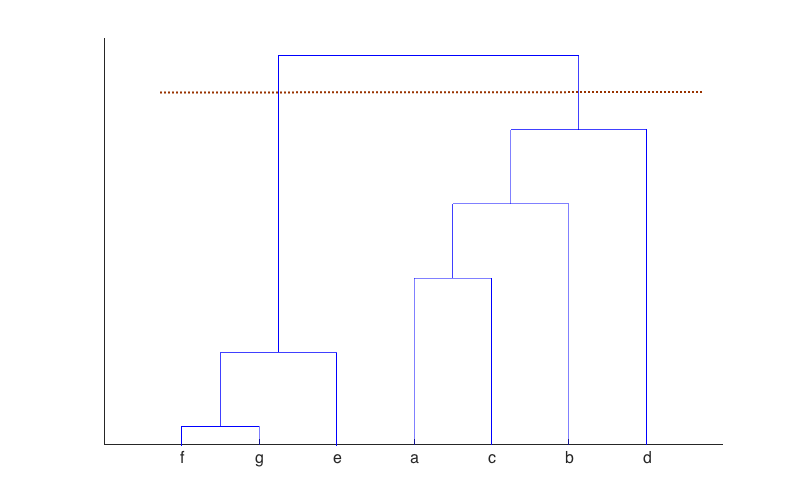
\includegraphics[width=3.5in]{figure/dendrogram_greedy}
	\caption{Dendrogram result of greedy algorithm}
	\label{fig:dendrogram_greedy}
\end{figure*}
%-------------------------------------------------------------------------------------
\subsection{Spectral Modularity Maximization Optimization Algorithm}
The spectral modularity maximization optimization algorithm is proposed by \citet{newman2006modularity}. This algorithm implies that modularity can be represented as the eigenvectors of  the modularity matrix, a characteristic matrix for the network, and applies a spectral method on this expression to obtain a high-quality community detection for the network. For each step, the algorithm divides the network into two communities based on the sign of the leading eigenvector and then repeats the process on the two communities. So first we introduce how to divide a network into two communities. This algorithm applies a different approach to define the modularity. Unlike the original one, \citet{newman2006modularity} supposes dividing a network into two communities and represents such a division by the quantities as follow:
\begin{equation}
s_{i} = \begin{cases}
+1 & \mbox{if vertex i belongs to community 1} \\
-1 & \mbox{if vertex i belongs to community 2} \\
\end{cases}
\end{equation}
So if vertex i and j are in the same community, $\frac{1}{2}(s_{i}s_{j} + 1)$ is 1, otherwise the value is 0. Based on this, the modularity can be represented as follows
\begin{equation}
Q  = \frac{1}{2m}(A_{ij} - \frac{k_{i}k_{j}}{2m})(s_{i}s_{j} + 1) = \frac{1}{4m}(A_{ij} - \frac{k_{i}k_{j}}{2m})s_{i}s_{j}
\end{equation}
This equation can be written in matrix form as
\begin{equation}
Q = \frac{1}{4m}s^{T}Bs
\label{equ:matrix form}
\end{equation}
where \textbf{s} is the column vector with $s_{i}$ as the elements. And B is called the modularity matrix, a real symmetric matrix whose elements are
\begin{equation}
	B_{ij} = A_{ij} - \frac{k_{i}k_{j}}{2m}
\label{equ:modularity matrix}
\end{equation}
The goal of the algorithm is to find a good division of the network that gets the highest modularity, which means we need to find the maximum value of equation \ref{equ:matrix form} for a given modularity matrix B. To satisfy this purpose, let $u_{i}(i = 1 , \cdots n)$ be  eigenvectors of B with eigenvalue $\beta_{i}$ for vector $u_{i}$(Assume $\beta_{1} \geq \beta_{2} \geq \beta_{2} \geq \cdots \geq \beta_{k}$). So \textbf{s} can be written as $s = \sum_{i}^{n}a_{i}u_{i}$, where $a_{i} = u_{i}^{T} \cdot s$. Now the equation \ref{equ:matrix form} can be transformed as follows
\begin{equation}
\begin{split}
Q & = \frac{1}{4m}s^{T}Bs \\
& = \frac{1}{4m}(\sum_{i}a_{i}u_{i}^{T})B(\sum_{j}a_{j}u_{j}) \\
& = \frac{1}{4m}(\sum_{i}\sum_{j}a_{i}a_{j}u_{i}^{T}Bu_{j})
\end{split}
\end{equation}
As $u_{i}$ and $\beta_{i}$ are the corresponding eigenvector and eigenvalue of B, we have $Bu_{i} = \beta_{i}u_{i}$. Besides, due to the distinct eigenvectors of the symmetric matrix are orthogonal. Therefor, if $i \neq j$,  the value of $u_{i}^{T}Bu_{j}$ is 0. Then the formulation of modularity can be simplified as follows
\begin{equation}
Q = \frac{1}{4m}(\sum_{i}(u_{i}^{T}s)^{2}\beta_{i})
\label{equ:final modularity}
\end{equation}
So, to get the highest modularity by choosing an appropriate clustering of the network, we hope to find a \textbf{s} to gain as much value as possible for the sum in equation \ref{equ:final modularity}. If there are no other restrictions, this problem could be solved easily by choosing the \textbf{s}, which is parallel to the $u_{1}$, which is the leading eigenvector of the modularity matrix \cite{newman2010networks}. This promise the largest eigenvalue $\beta_{1}$ is involved in the sum and the other terms in the equation are automatically zero, because the eigenvectors of the symmetric matrix  are orthogonal to each other. While, unfortunately, there is a restriction that the value of $s_{i}$ should be 1 or -1, which means \textbf{s} would not be easily selected parallel to $u_{1}$. So the best we can do is to make \textbf{s} as close parallel as possible to $u_{1}$. In others words, we should keep the dot product $u_{1}^{T}\cdot s$ be the highest value. To maximize the dot product, we should let $s_{i} = 1$ if the corresponding element of $u_{1}$ is positive, otherwise $s_{i} = -1$. Then based on the sign of $s_{i}$, we would divide the whole network into two communities. The positive value is one community and the negative ones compose another one. Here is an example displays how this algorithm divides a network into two communities.For the network shown in figure \ref{fig:exp spectral}, based on equation \ref{equ:modularity matrix} we constructed the modularity matrix B, as shown in Figure \ref{equ:exp modularity matrix}. Then based on the modularity matrix, we calculated the leading vector(see Figure \ref{equ:exp leading vector}) of this modularity matrix. At last,  based on the sign of leading vector, we can divide the network into two parts, which is shown in figure \ref{fig:result of spectral}. We can see that the clustering result is same as the one we have obtained by the greedy modularity maximization optimization algorithm.
\begin{figure*}
	\centering
	\resizebox{2.5in}{!}{
		\begin{tikzpicture}
		\node(a) at (-2,2)[node]{a};
		\node(b) at (2,2)[node]{b};
		\node(c) at (-2,-2)[node]{c};
		\node(d) at (2,-2)[node]{d};
		\node(e) at (6,0)[node]{e};
		\node(f) at (8,2)[node]{f};
		\node(g) at (8,-2)[node]{g};
		\draw[arrow4] (a) -- (b);
		\draw[arrow4] (a) -- (c);
		\draw[arrow4] (b) -- (c);
		\draw[arrow4] (b) -- (d);
		\draw[arrow4] (b) -- (e);
		\draw[arrow4] (c) -- (d);
		\draw[arrow4] (d) -- (e);
		\draw[arrow4] (e) -- (f);
		\draw[arrow4] (e) -- (g);
		\draw[arrow4] (f) -- (g);
		\end{tikzpicture}}
	\caption{Example for spectral modularity optimization algorithm}
	\label{fig:exp spectral}
\end{figure*}

\begin{figure*}
	\centering
	\resizebox{2.8in}{!}{
	\begin{minipage}{0.55\textwidth}
		\begin{equation*}
		B = \frac{1}{20}
		\begin{pmatrix}
		-4 & 12 & 14 & -6 & -8 & -4 & -4 \\
		12 & -16 & 8 & 8 & 4 & -8 & -8 \\
		14 & 8 & -9 & 11 & -12 & -6 & -6 \\
		-6 & 8 & 11 & -9 & 8 & -6 & -6 \\
		-8 & 4 & -12 & 8 & -16 & 12 & 12 \\
		-4 & -8 & -6 & -6 & 12 & -4 & 16 \\
		-4 & -8 & -6 & -6 & 12 & 16 & -4 
		\end{pmatrix}
		\end{equation*}
		\caption{Modularity matrix}
		\label{equ:exp modularity matrix}
	\end{minipage}}
		\resizebox{2in}{!}{
			\begin{minipage}{0.4\textwidth}
				\begin{equation*}
				Leading ~ eigenvector = 
				\begin{pmatrix}
				-0.37 \\
				-0.30 \\
				-0.43 \\
				-0.17 \\
				0.32 \\
				0.48 \\
				0.48
				\end{pmatrix}
				\end{equation*}
				\caption{Leading eigenvector}
				\label{equ:exp leading vector}
			\end{minipage}}
\end{figure*}

\begin{figure*}
	\centering
	\resizebox{2.6in}{!}{
		\begin{tikzpicture}
		\node(a) at (-2,2)[node]{a};
		\node(b) at (2,2)[node]{b};
		\node(c) at (-2,-2)[node]{c};
		\node(d) at (2,-2)[node]{d};
		\node(e) at (6,0)[node]{e};
		\node(f) at (8,2)[node]{f};
		\node(g) at (8,-2)[node]{g};
		\draw[arrow4] (a) -- (b);
		\draw[arrow4] (a) -- (c);
		\draw[arrow4] (b) -- (c);
		\draw[arrow4] (b) -- (d);
		\draw[arrow4] (b) -- (e);
		\draw[arrow4] (c) -- (d);
		\draw[arrow4] (d) -- (e);
		\draw[arrow4] (e) -- (f);
		\draw[arrow4] (e) -- (g);
		\draw[arrow4] (f) -- (g);
		\draw[red,dotted, line width = 1pt] (0,0) circle (3.5);
		\draw[red,dotted, line width = 1pt] (7.2,0) ellipse (2 and 3.5);
		\end{tikzpicture}}
	\caption{Result of spectral modularity optimization algorithm}
	\label{fig:result of spectral}
\end{figure*}

However, in the real world, most of the networks contain more than two communities, so we extend the spectral modularity maximization optimization algorithm to find appropriate divisions of the network into several communities. To address this problem, we first divide the network into two subnetworks and then repeatedly apply the algorithm on the subnetwork divided by the last step and compute the additional modularity $\bigtriangleup Q$ for each division. Suppose dividing a network n of size $l_{n}$ into two subnetworks, the additional modularity to the whole modularity is
\begin{equation}
	\bigtriangleup Q = \frac{1}{2m}[\frac{1}{2}\sum_{i,j \in n}B_{ij}(s_{i}s_{j} + 1) - \sum_{i,j \in n}B_{ij} ]
\end{equation}

As $\sum_{i,j \in c}B_{ij} = \sum_{i,j\in c}s_{i}s_{j}\delta_{ij}\sum_{k\in c}B_{ik}$ and let $\omega_{ij} = 1$ if i = j, otherwise is 0, the equation can be simplified as follows
\begin{equation}
\begin{split}
\bigtriangleup Q & = \frac{1}{2m}[\frac{1}{2}\sum_{i,j \in n}B_{ij}(s_{i}s_{j} + 1) - \sum_{i,j \in n}B_{ij} ] \\
& =  \frac{1}{4m}[\frac{1}{2}\sum_{i,j \in c}B_{ij}s_{i}s_{j} - \sum_{i,j \in c}B_{ij} ]\\
& = \frac{1}{4m}\sum_{i,j \in c}[B_{ij} - \omega_{ij} \sum_{k \in c}B_{ik}]s_{i}s_{j} \\
& = \frac{1}{4m}s^{T}B^{(n)}s
\end{split} 
\label{equ:spectral modularity more than two}
\end{equation}
where  $B^{(n)}$ is the matrix of size $l_{n} \times l_{n}$ with elements which is indexed by the label i,j of nodes in network n and having weights
\begin{equation}
B_{ij}^{(g)} = B_{ij} - \omega_{ij}\sum_{k \in g} B_{ik}
\end{equation}
We noticed that equation \ref{equ:spectral modularity more than two} has the same form of equation \ref{equ:matrix form}, so we also apply the spectral method to maximize $\bigtriangleup Q $ of the generalized modularity matrix. If there is no positive value of $\bigtriangleup Q $, the subgroup is indivisible. Thus the algorithm is shown as Algorithm 2: 
\begin{algorithm}
	\caption{Spectral Modularity Maximization Algorithm}
	Construct the modularity matrix for the network\;
	\Repeat{find the split make no positive contribution to the total modularity}{
		Find the leading eigenvalue and corresponding eigenvector of the modularity matrix\;
		Add the change of modularity to the total modularity\;
		Divide the network into two communities based on the signs of the elements of the eigenvector\;
		Construct the modularity matrix for the subnetwork\;}
\end{algorithm}
%-------------------------------------------------------------------------------------
\section{Evaluation measures}
We use two categories of evaluation measure. One is F-measure \cite{wagner2007comparing}, which is based on the cluster matching. Another is Rand Index(RI) \cite{rand1971objective}, which is based on the pair counting. We use programming language labeled by GitHub as the ground truth. 
%-------------------------------------------------------------------------------------
\subsection{F-measure}
F-measure \cite{wagner2007comparing} is usually used to measure the similarity between to partitions. Its value depends on the combination of precision and recall. Precision is the percentage of selected items that are correct and recall represents the percentage of correct items that are selected. Suppose Figure \ref{fig:F-measure} is a network, $C = \{C_{1}, \cdots C_{k}\}$ is the ground truth for network and $C' = \{C'_{1}, \cdots C'_{k}\}$ represents a clustering for the network. So the precision for each pair of $C_{i}$ and $C'_{j}$ 
\begin{figure*}
	\centering
	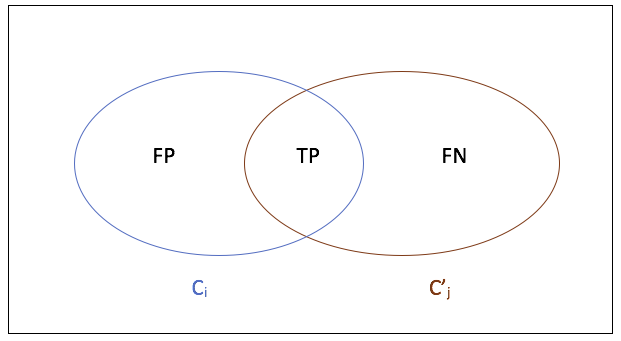
\includegraphics[width=3in,keepaspectratio]{figure/F_measure}
	\caption{F-measure}
	\label{fig:F-measure}
\end{figure*}
\begin{equation}
	Precision = \frac{TP}{TP + FP} = \frac{|C_{i} \cap C'_{j}|}{|C_{i}|}
\end{equation}
and recall is 
\begin{equation}
	Recall = \frac{TP}{TP + FN} = \frac{|C_{i} \cap C'_{j}|}{|C'_{j}|}
\end{equation}
Then we get the F-measure for $C_{i}$ and $C'_{j}$ is
\begin{equation}
	\mbox{F-measure}(C_{i}, C'_{j}) = \dfrac{2 \cdot Precision \cdot Recall}{Precision + Recall} = \dfrac{2 \cdot |C_{i} \cap C'_{j}|}{|C_{i} + C'_{j}|}
	\label{equ:F-measure}
\end{equation}
So the overall F-measure is the weighted sum of the maximum F-measures for clusters $C$:
\begin{equation}
\mbox{F-measure}(C,C') = \frac{1}{|V|}\sum_{c_{i}\in C}|c_{i}|\max_{c'_{j}\in C'}\frac{2|c_{i}\cap c'_{j}|}{|c_{i}|+|c'_{j}|} 
\end{equation}
\begin{figure*}
	\centering
	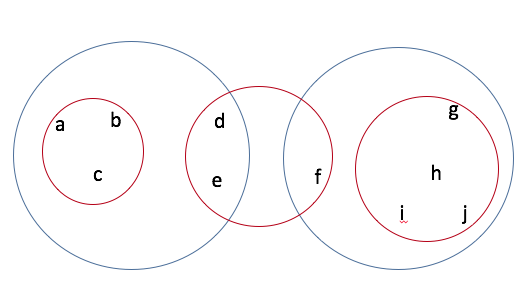
\includegraphics[width=3in,keepaspectratio]{figure/Fmeasure_example}
	\caption{Example of F-measure}
	\label{fig:F-measure example}
\end{figure*}

Here is an example(see Figure \ref{fig:F-measure example}) explain how to calculate the F-measure. In the example, there are 10 vertices. The blue circles represent the clusters of ground truth and the red  circles are the clusters we have got. So we have C : $c_{1}\{a,b,c,d,e\}$, $c_{2} \{f,g,h,i,k \}$ and $C'$: $c'_{1}\{ a,b,c\}$, $c'_{2} \{d,e,f\}$ , $c'_{3} \{g,h,i,k\}$. So based on equation \ref{equ:F-measure}, we calculate the F-measure of each pair of C and $C'$ and result is shown as follows
\begin{equation*}
	\frac{2|c_{1}\cap c'_{1}|}{|c_{1}|+|c'_{1}|} = \frac{2 \times 3}{5 + 3} = \frac{3}{4}   \qquad	\frac{2|c_{1}\cap c'_{2}|}{|c_{1}|+|c'_{2}|} = \frac{2 \times 2}{5 + 3} = \frac{1}{2}  \qquad 
	\frac{2|c_{1}\cap c'_{4}|}{|c_{1}|+|c'_{4}|} = \frac{2 \times 0}{5 + 4} = 0
\end{equation*}
\begin{equation*}
	\frac{2|c_{2}\cap c'_{1}|}{|c_{2}|+|c'_{1}|} = \frac{2 \times 0}{5 + 3} = 0   \qquad   \frac{2|c_{2}\cap c'_{2}|}{|c_{2}|+|c'_{2}|} = \frac{2 \times 1}{5 + 3} = \frac{1}{4} \qquad
	\frac{2|c_{2}\cap c'_{3}|}{|c_{2}|+|c'_{3}|} = \frac{2 \times 4}{5 + 4} = \frac{8}{9}
\end{equation*}
So the overall F-measure of clustering C' is  
\begin{equation*}
\mbox{F-measure}(C, C') = \frac{1}{10} (5 \times \frac{3}{4} + 5 \times \frac{8}{9} ) \approx 0.82
\end{equation*}
%-------------------------------------------------------------------------------------
\subsection{Rand Index}
Rand Index \cite{rand1971objective} is also a measure used to evaluate the similarity between two clusterings. Unlike F-measure, rand index considers the pair of vertices. It represents the fraction of the number of vertex pair which is clustered in the same ways in both clusterings to the total number of pairs. So errors only happen under two situations. One is two vertices belonging to the same community are assigned to different communities after clustering and another is two vertices belonging to different communities are assigned to the same community.
\begin{table*}[h]
	\centering
	\begin{tabular}{|c c|c c|} \hline
		& & \multicolumn{2}{|c|}{Ground Truth} \\  
		& & $C(v_{i}) = C(v_{j})$ &  $C(v_{i}) \neq C(v_{j})$ \\ \hline
		Clustering &  $C'(v_{i}) = C'(v_{j})$ & $ a_{11} $ & $a_{10}$ \\ 
		Result & $C'(v_{i}) \neq C'(v_{j})$ & $ a_{01} $ & $a_{00}$ \\ \hline
	\end{tabular}
	\caption{Rand index}
	\label{tab:rand index}
\end{table*}

Suppose C represents the ground truth of a network and $C'$ is a clustering for the same network.  As Table \ref{tab:rand index} shown, $a_{11}$ represent the number of pair of vertices that are in the same clusters in both the ground truth and the partition. $a_{10}$ indicates the count of pairs of vertices that are in the different communities of the ground truth but in the same community for in partition C'. $a_{01}$ denote the number of pairs of vertices that in the same community of ground truth which are in different communities in C'. And $a_{00}$ be the number of pairs of vertices which are in different clusters for both ground truth C and clusters C'. So $A = a_{11} + a_{01} + a_{10} + a_{00}$ is the total number of pairs of vertices in the network. So the rand index is 
\begin{equation}
Rand ~ Index = \frac{a_{11} + a_{00}}{a_{11} + a_{01} + a_{10} + a_{00}}
\end{equation}
%-------------------------------------------------------------------------------------
%In this chapter, we firstly introduce three different weighting schemes, dot product, cosine similarity and Jaccard similarity and we used these weighting schemes to transform the heterogeneous network to the homogeneous network. Then, we explain the inverse document frequency,which is used to reduce the effect of users who participate a large number of repositories. Next, we describe the theory of two clustering algorithms based on the modularity. One is the greedy modularity maximization optimization algorithm and another one is spectral modularity maximization optimization algorithm. At last, we introduce the evaluation measures that will be used in our experiments, F-measure and rand index.
%-------------------------------------------------------------------------------------
\section{Clustering Results}
In this subsection, we introduced the experiment we have done to study the interaction between different weighting schemes and clustering algorithms. In my experiments, we extracted four subnetworks(Python \& HTML, Objective-C \& C, PHP \& CSS and Java \& Ruby), which only includes two categories of programming language repository, from both repository-contributor network and repository-stargazer network. Then we transformed the heterogeneous subnetwork into the homogeneous network, which only includes repositories, by using three weighting schemes, dot product, cosine similarity and Jaccard similarity. In addition, we also applied the inverse document frequency on the original heterogeneous network to reduce the effect of those users, who participate too many repositories, and then transformed the new network by dot product and cosine similarity, because Jaccard similarity is only available for binary one. At last, we separately applied the greedy modularity optimization algorithm and spectral modularity optimization algorithm to cluster the homogeneous network. As we have already known that each dataset only includes two kinds of repositories, we just cluster the network into two communities and  evaluate the performance of different weighing schemes by F-measure and rand Index with ground truth. In addition, we also analyzed those repositories that are clustered into the wrong communities to find out the reason. 

In my experiments, I have implemented the process of data crawling, extraction of subnetworks, network transformation, and network clustering. All of the code is written in Python. Except the implementation of greedy modularity maximization optimization algorithm, I used the function community\_fastgreedy of igraph \cite{igraph}, all the other code is original.
%-------------------------------------------------------------------------------------
 \subsection{Visualization of the Original Clusters}
Before running the clustering algorithm, we visualized the clusters using labeled data. First, we transformed the repository-user networks to repository networks using three weighting schemes, dot product, cosine similarity and Jaccard similarity. In addition, to reduce the effect of users that participate in a large number of repositories, we also applied the inverse document frequency on the repository-user subnetworks and then transformed the new heterogeneous network to the homogeneous one. As Jaccard similarity is only available for the binary object, we just utilized dot product and cosine similarity to complete the transformation. Now we have obtained the repository network and to visualize the repository networks, firstly, we used Gephi \cite{bastian2009gephi} and Figure \ref{fig:Gephi visualization of Objective-C and C repository-stargazer networks} is an example of the repository network transformed from Objective-C and C repository-stargazer network. From the figure, we can see that although we have already applied the function of preventing overlap, there is still a lot of vertices overlap and we also noticed that the red vertices are located close to each other, while the blue vertices are distributed dispersedly. In addition, after we applied the inverse document frequency, the two kinds of vertices are mixed together and it is impossible to find a borderline between them. The reason cause this is that the layout of the Gephi graph is one dimensional. To ameliorate this problem, we use Largevis\cite{tang2016visualizing} to visualize the networks. Largevis takes a weighted graph as input and utilizes node embedding technology and represents each vertex using a vector. Then it reduces vector length to two dimensions to implement network visualization.
\begin{figure*}
	\centering
	\subcaptionbox{Dot product}{
		\includegraphics[width = 1.8 in]{figure/OC_intersection}}
	\subcaptionbox{Cosine}{
		\includegraphics[width = 1.8 in]{figure/OC_cosine}}
	\subcaptionbox{Jaccard}{
		\includegraphics[width = 1.8 in]{figure/OC_Jaccard}}
	\subcaptionbox{Dot product \& IDF}{
		\includegraphics[width = 1.8 in]{figure/OC_idf_intersection}}
	\subcaptionbox{Cosine \& IDF}{
		\includegraphics[width = 1.8 in]{figure/OC_idf_cosine}}
	\caption{Gephi visualization of Objective-C and C repository-stargazer networks}
	\label{fig:Gephi visualization of Objective-C and C repository-stargazer networks}
\end{figure*}

 As the weighted repository network could be represented as a square matrix and each repository could be represented as a vector, whose element is the distance between this repository to the others, reducing the vector length to two dimensions by Largevis, we get the coordinates of each repository. Then we plot the repository based on the coordinates by Matlab and Figure \ref{fig:repository distribution of repository-contributor} and Figure \ref{fig:repository distribution of repository-stargazer} display the distribution of repositories of repository-contributor subnetworks and repository-stargazer subnetworks that transformed by different weighting schemes, respectively. From Figure \ref{fig:repository distribution of repository-contributor}, we found that for all subnetworks of repository-contributor network, no matter which weighting schemes we selected or whether applied the inverse document frequency or not, after the transformation, most of the repositories are distributed together. But there are also some repositories are located away from the principal part and after checking these repositories, we found that there is no connection between these repositories and the principal part and these repositories are usually only connected with one repository, which is also far away from the main part. And for the main part, in most cases, we can clearly distinguish two kinds of repositories as there is a clear borderline between two communities. While, there are some special cases that two categories are distributed together so that it is difficult to cluster, such as the Python and HTML network transformed by the combination of cosine similarity and inverse document frequency. 

Unlike the repository-contributor subnetworks, for all weighting schemes, the repositories of all repository subnetworks, obtained by the subnetworks extracted from repository-stargazer network, are clearly distributed into two regions and there is only a few number of repositories are distributed into the incorrect communities. In addition, we found that after applying the inverse document frequency, the distribution of repositories is more sparsely. Therefore, comparing the distribution of two kinds of subnetworks, we could get better clustering results of repository subnetworks transformed by the repository-stargazer network than those transformed by the repository-contributor subnetworks.
\begin{figure*}
	\centering
	\subcaptionbox{Dot product}{
		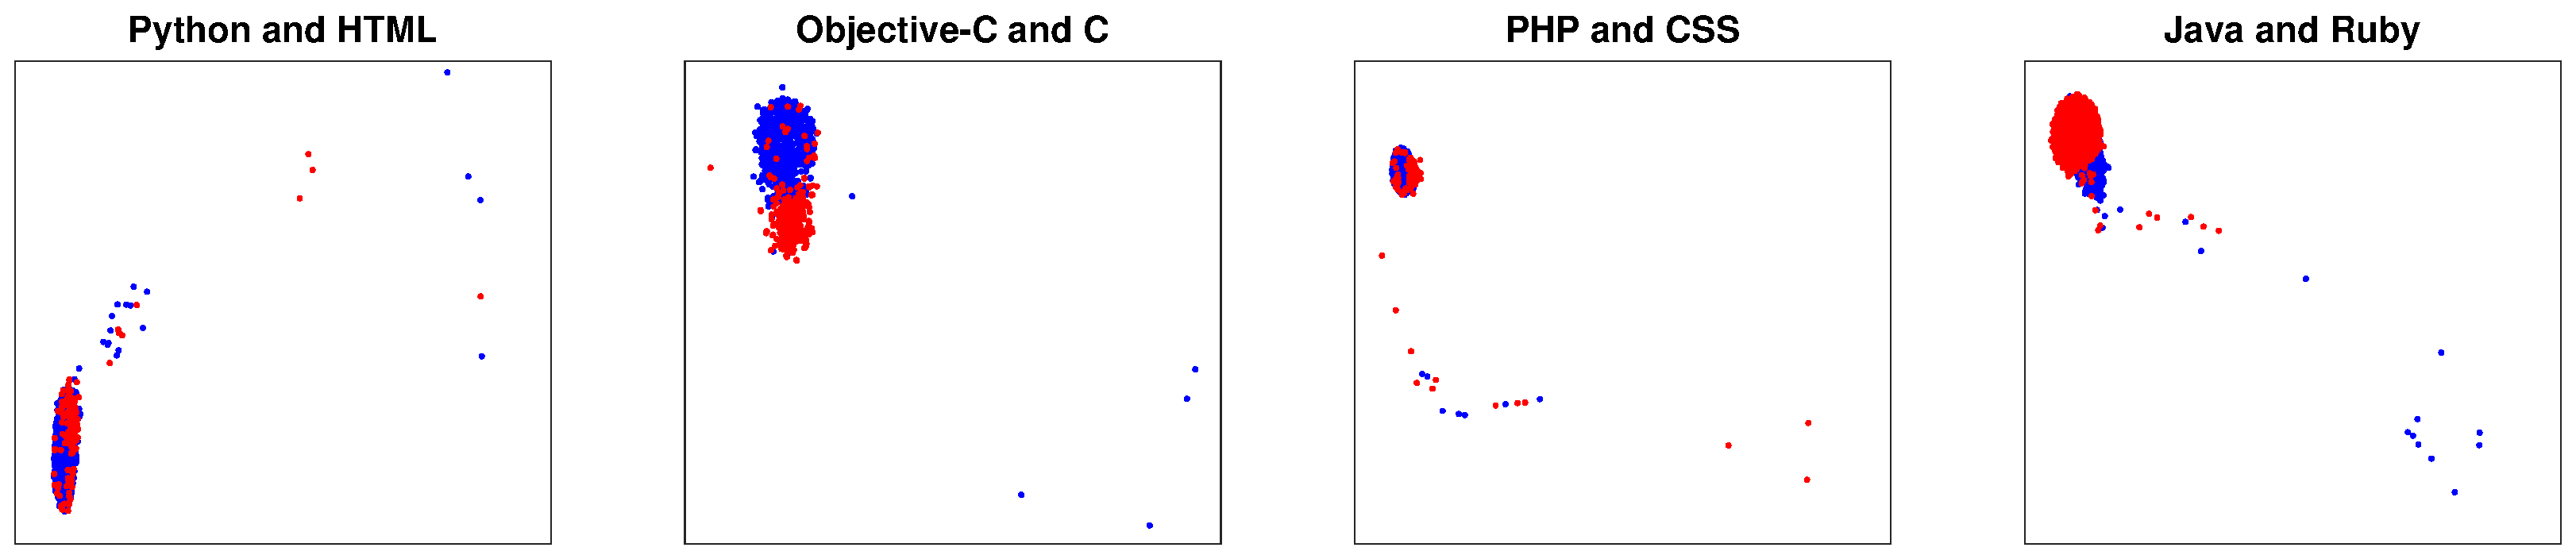
\includegraphics[width = 6 in]{figure/con_intersection.eps}}
	\subcaptionbox{Cosine}{
		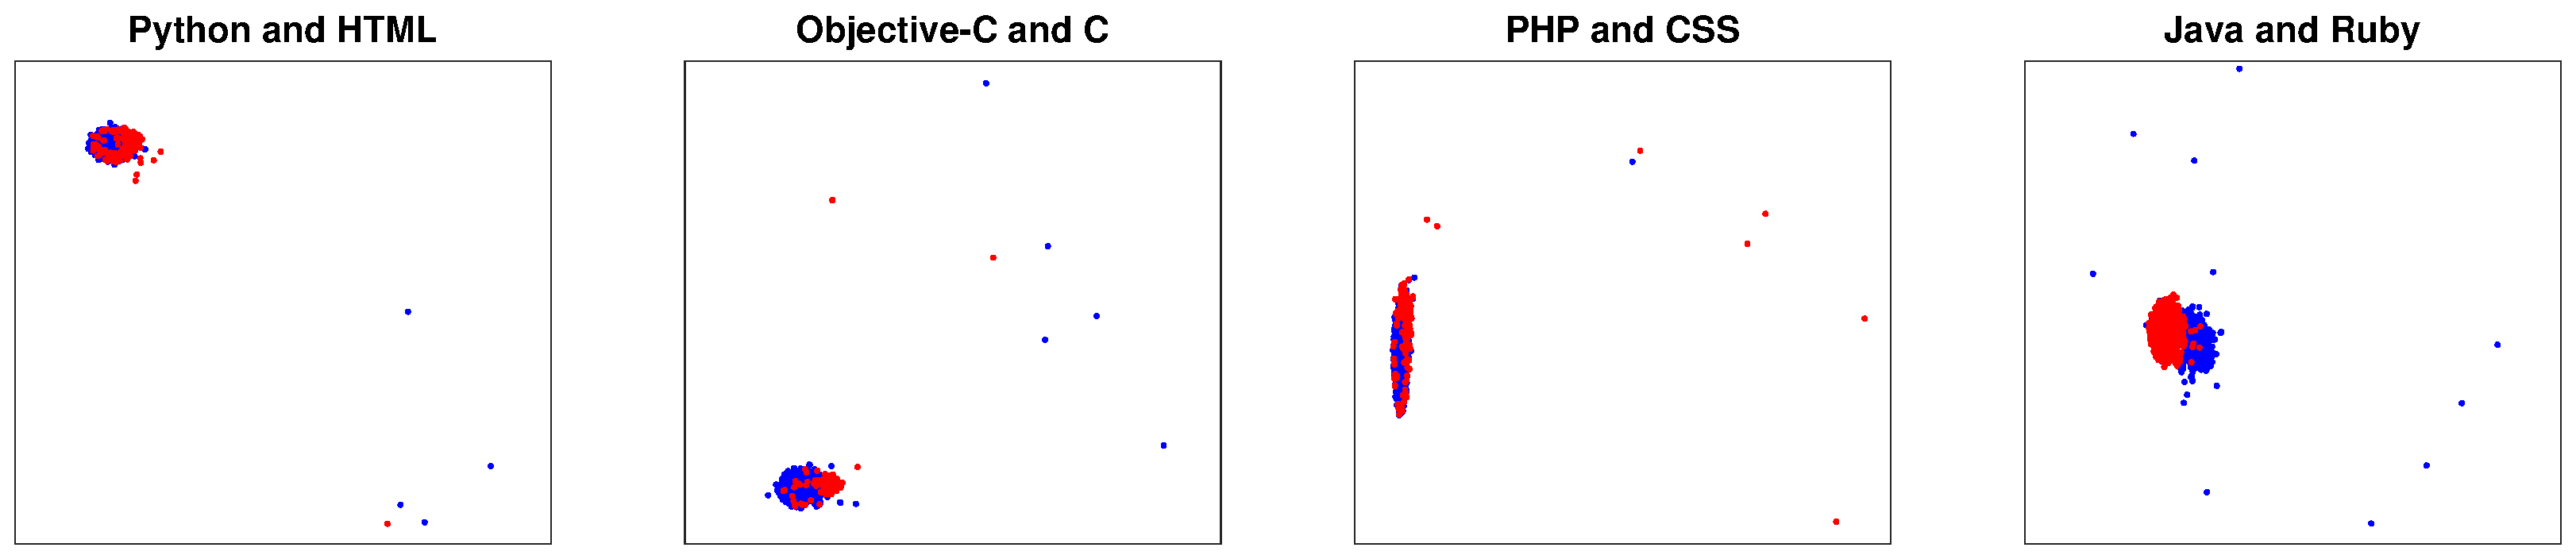
\includegraphics[width = 6 in]{figure/con_cosine.eps}}
	\subcaptionbox{Jaccard}{
		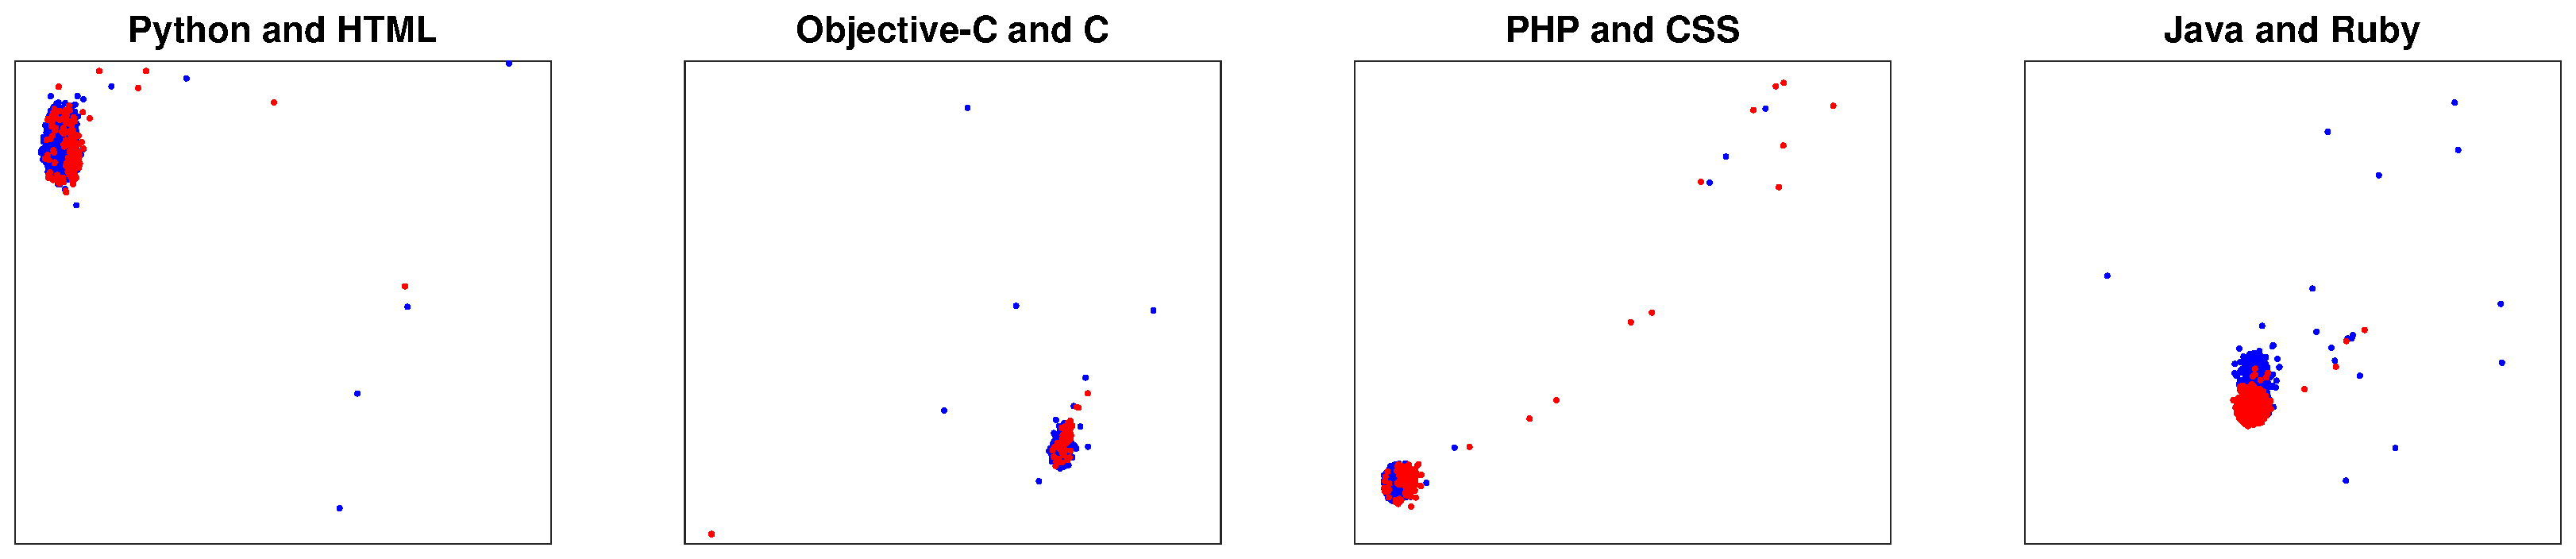
\includegraphics[width = 6 in]{figure/con_Jaccard.eps}}
	\subcaptionbox{Dot product + idf}{
		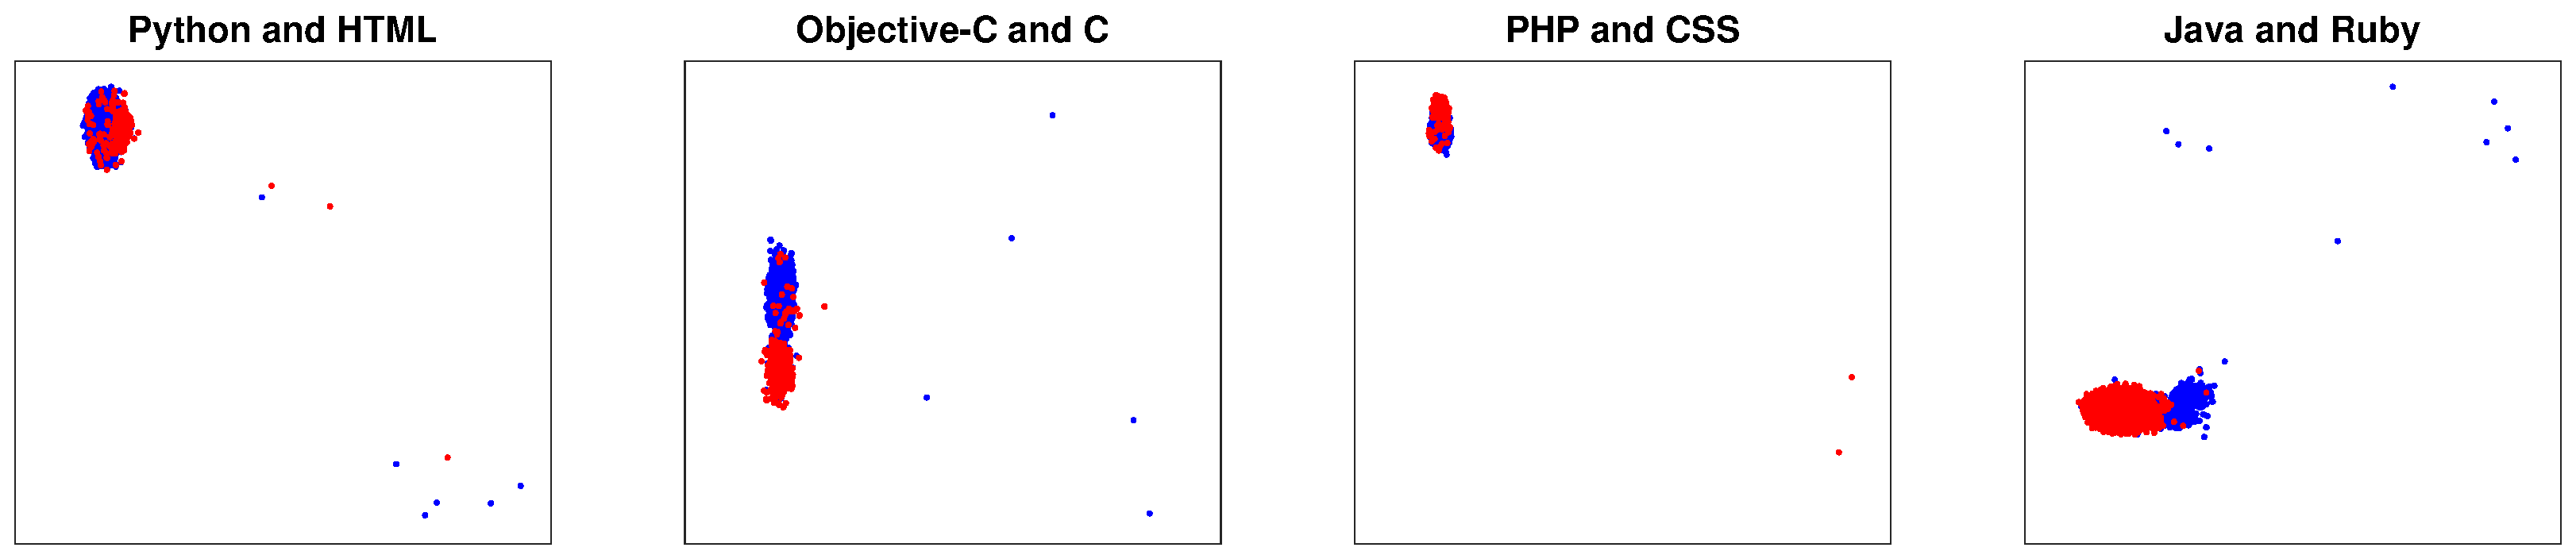
\includegraphics[width = 6 in]{figure/con_idf_intersection.eps}}
	\subcaptionbox{Cosine + idf}{
		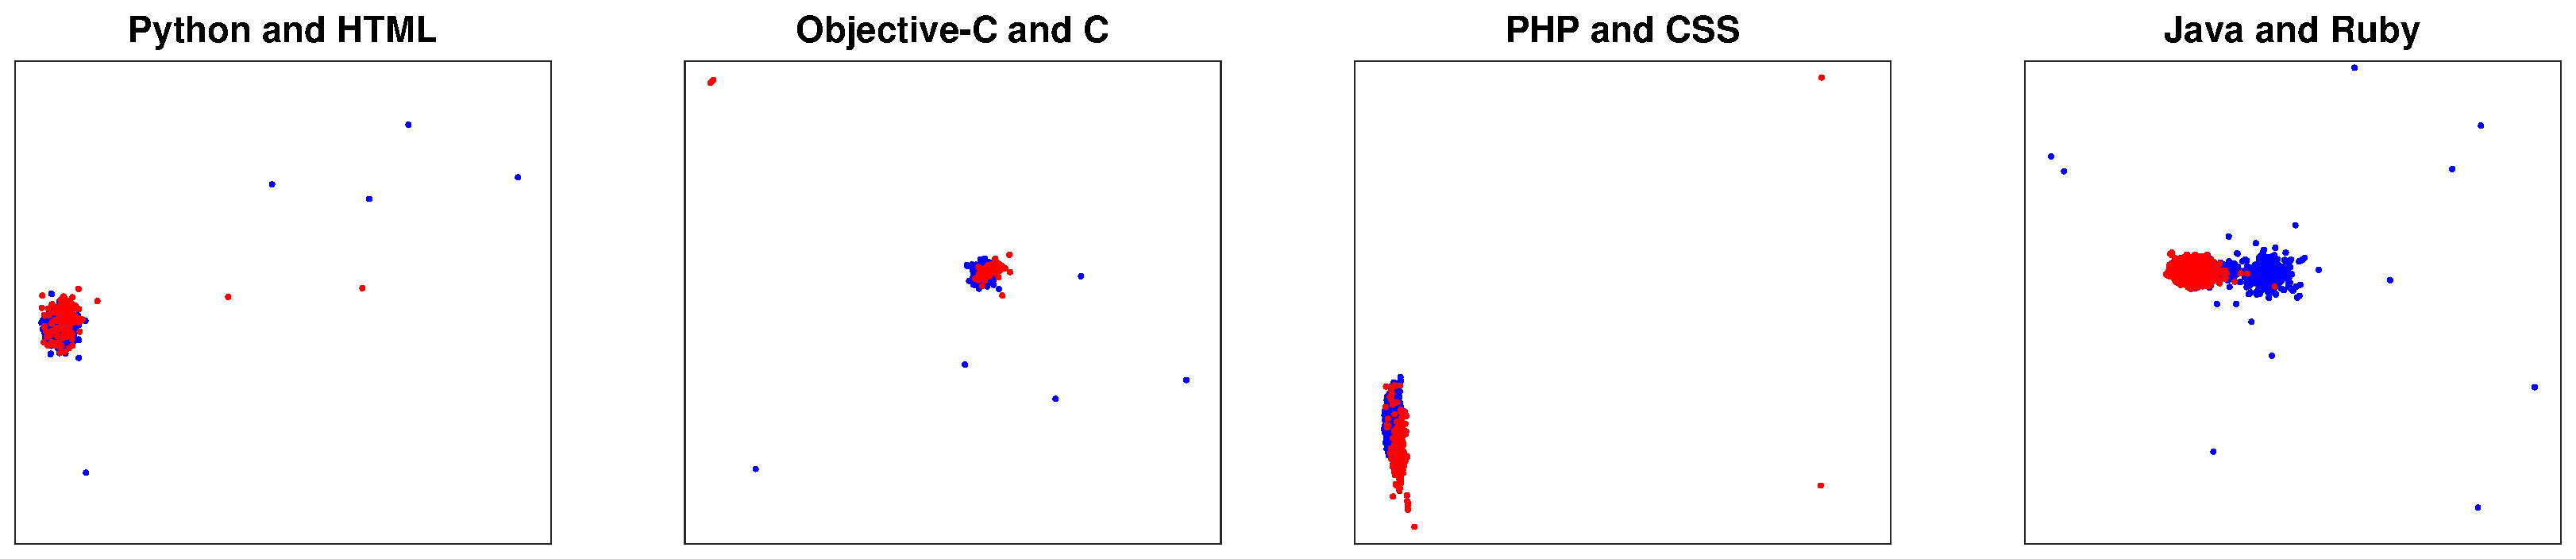
\includegraphics[width = 6 in]{figure/con_idf_cosine.eps}}
	\caption{Repository distribution of subnetworks transformed from repository-contributor networks}
	\label{fig:repository distribution of repository-contributor}
\end{figure*}


\begin{figure*}
	\centering
	\subcaptionbox{Dot product}{
		\includegraphics[width = 6 in]{figure/star_intersection.eps}}
	\subcaptionbox{Cosine}{
		\includegraphics[width = 6 in]{figure/star_cosine.eps}}
	\subcaptionbox{Jaccard}{
		\includegraphics[width = 6 in]{figure/star_Jaccard.eps}}
	\subcaptionbox{Dot product + idf}{
		\includegraphics[width = 6 in]{figure/star_idf_intersection.eps}}
	\subcaptionbox{Cosine + idf}{
		\includegraphics[width = 6 in]{figure/star_idf_cosine.eps}}
	\caption{Repository distribution of subnetworks transformed from repository-stargazer subnetworks}
	\label{fig:repository distribution of repository-stargazer}
\end{figure*}

\subsection{SubNetwork Clustering Results}
	Then we clustered these repository networks by two clustering algorithms, greedy modularity maximization optimization algorithm and spectral modularity maximization optimization algorithm. Based on the clustering results, we reordered the repositories of each repository network and plotted their relations for different weighting schemes. Figure \ref{fig:clustering result by greedy algorithm of repository-contributor network} and Figure \ref{fig:clustering result by spectral algorithm of repository-contributor network} separately display the clustering results of the repository network, obtained from the repository-contributor network, for greedy clustering algorithm and spectral clustering algorithm.  For the greedy algorithm, the figures of the same dataset are almost same. While, for the spectral algorithm, most of these figures also do not provide useful information and it is difficult to distinguish two communities from the figures. Table \ref{tab:evaluation result of repository-contributor network} displays the value of modularity and the evaluation measure values of community structures detected by the two clustering algorithms on these subnetworks. From the table, we noticed a strange phenomenon that no matter which weighting schemes we used to transform the repository-contributor network, the evaluation measures of the greedy algorithm is same for all four datasets. The result also explains why in Figure \ref{fig:clustering result by greedy algorithm of repository-contributor network} all the figures of the same dataset  are same. However, as the different weighting schemes we used, the modularity is different. We can see that without inverse document frequency, Jaccard similarity obtains the highest modularity, which is followed by cosine similarity and the value of dot product gets the lowest one. When we applied the inverse document frequency, the modularity of both dot product and cosine similarity increase and cosine similarity receives the highest modularity from all the weighting schemes. On the other hand, for the spectral algorithm, the combination of cosine similarity and inverse document frequency gets the highest value of both F-measure and rand index on Python and HTML dataset and PHP and CSS dataset. It also obtains higher F-measure(0.7510) than other weighing schemes on Objective-C and C dataset, but dot product receives the highest rand index(0.6323). For Java and Ruby, cosine similarity performs best for both evaluation measures. In addition, we found cosine similarity and Jaccard similarity gets higher modularity than dot product. Unlike the result of greedy algorithm, the inverse document frequency decreases the modularity for both dot product and cosine similarity. 
\begin{figure*}
	\centering
	\subcaptionbox{Dot product}{
		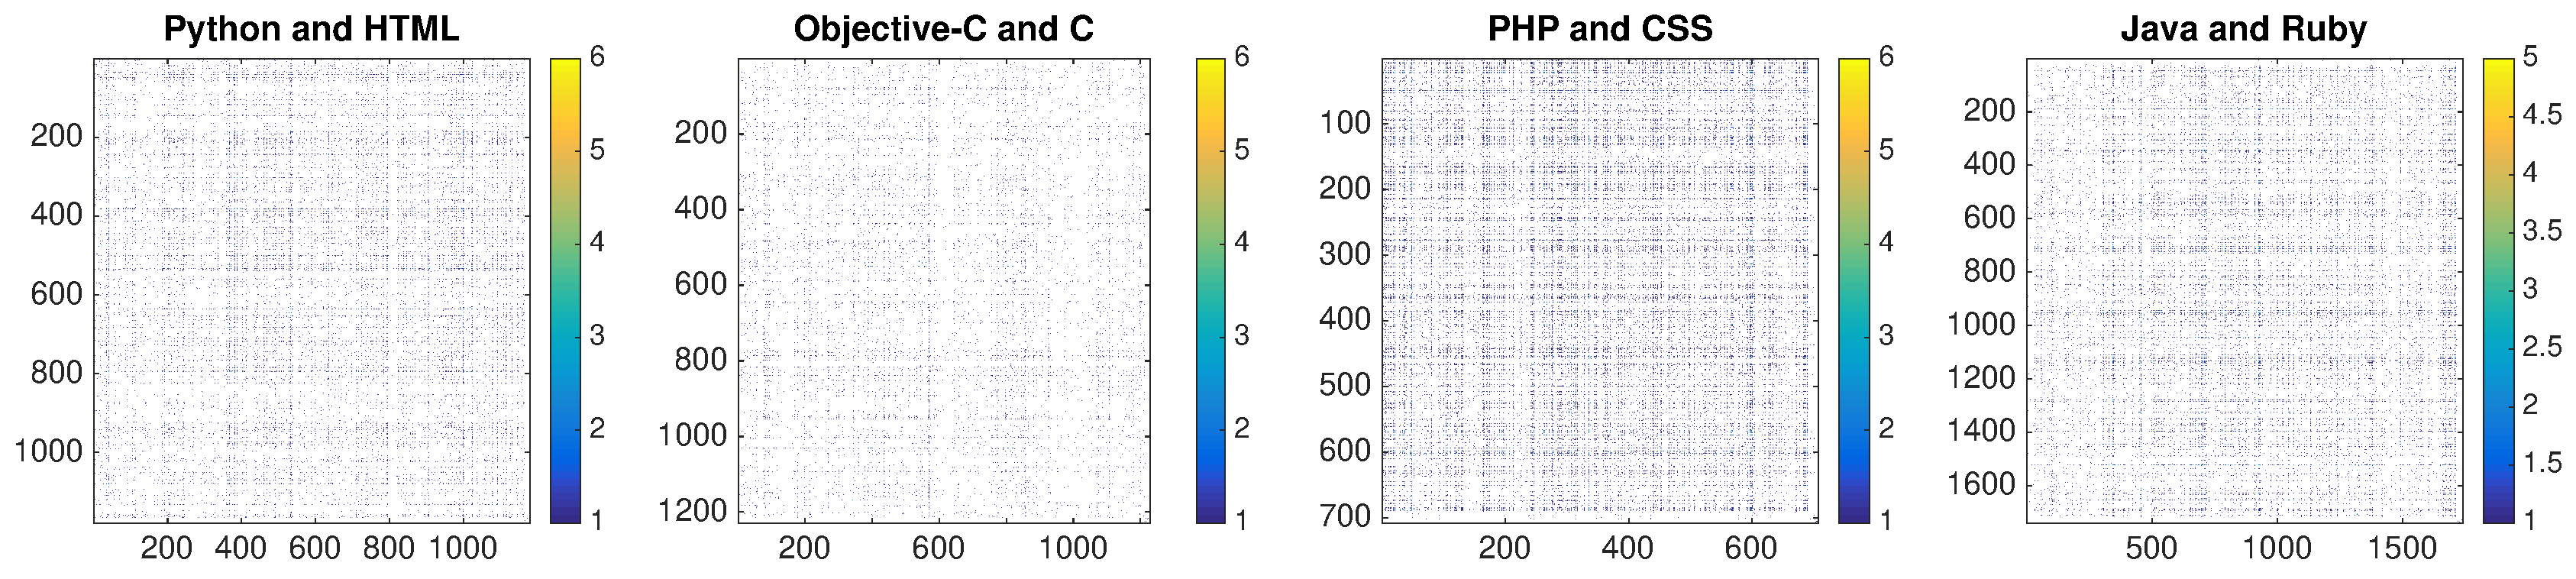
\includegraphics[width = 6 in]{figure/con_intersection_greedy.eps}}
	\subcaptionbox{Cosine}{
		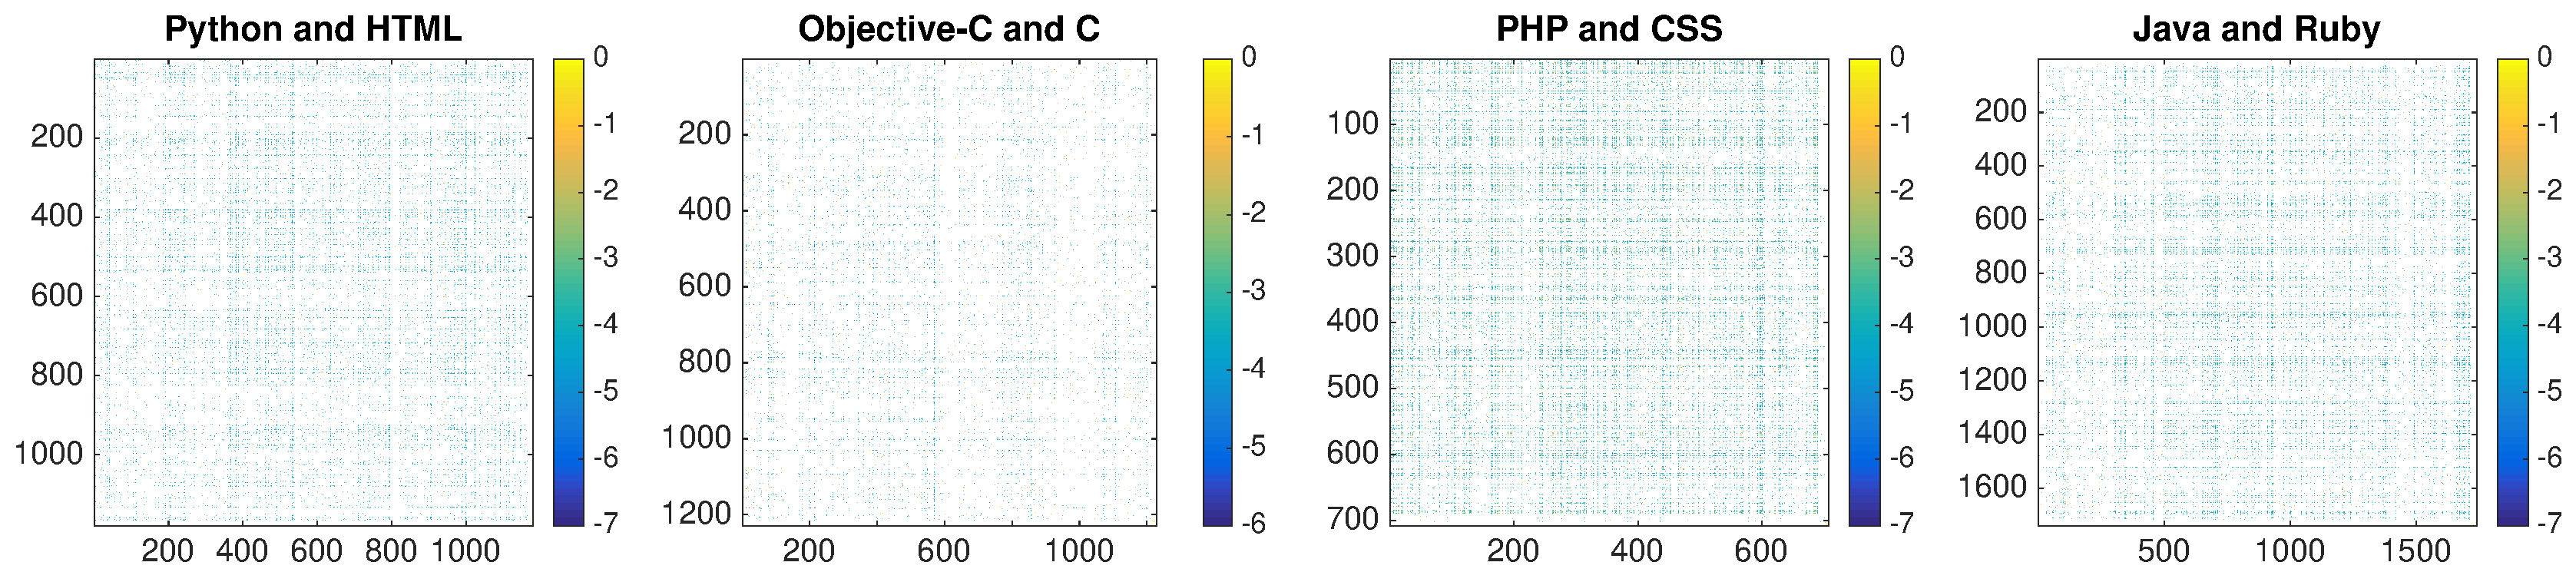
\includegraphics[width = 6 in]{figure/con_cosine_greedy.eps}}
	\subcaptionbox{Jaccard}{
		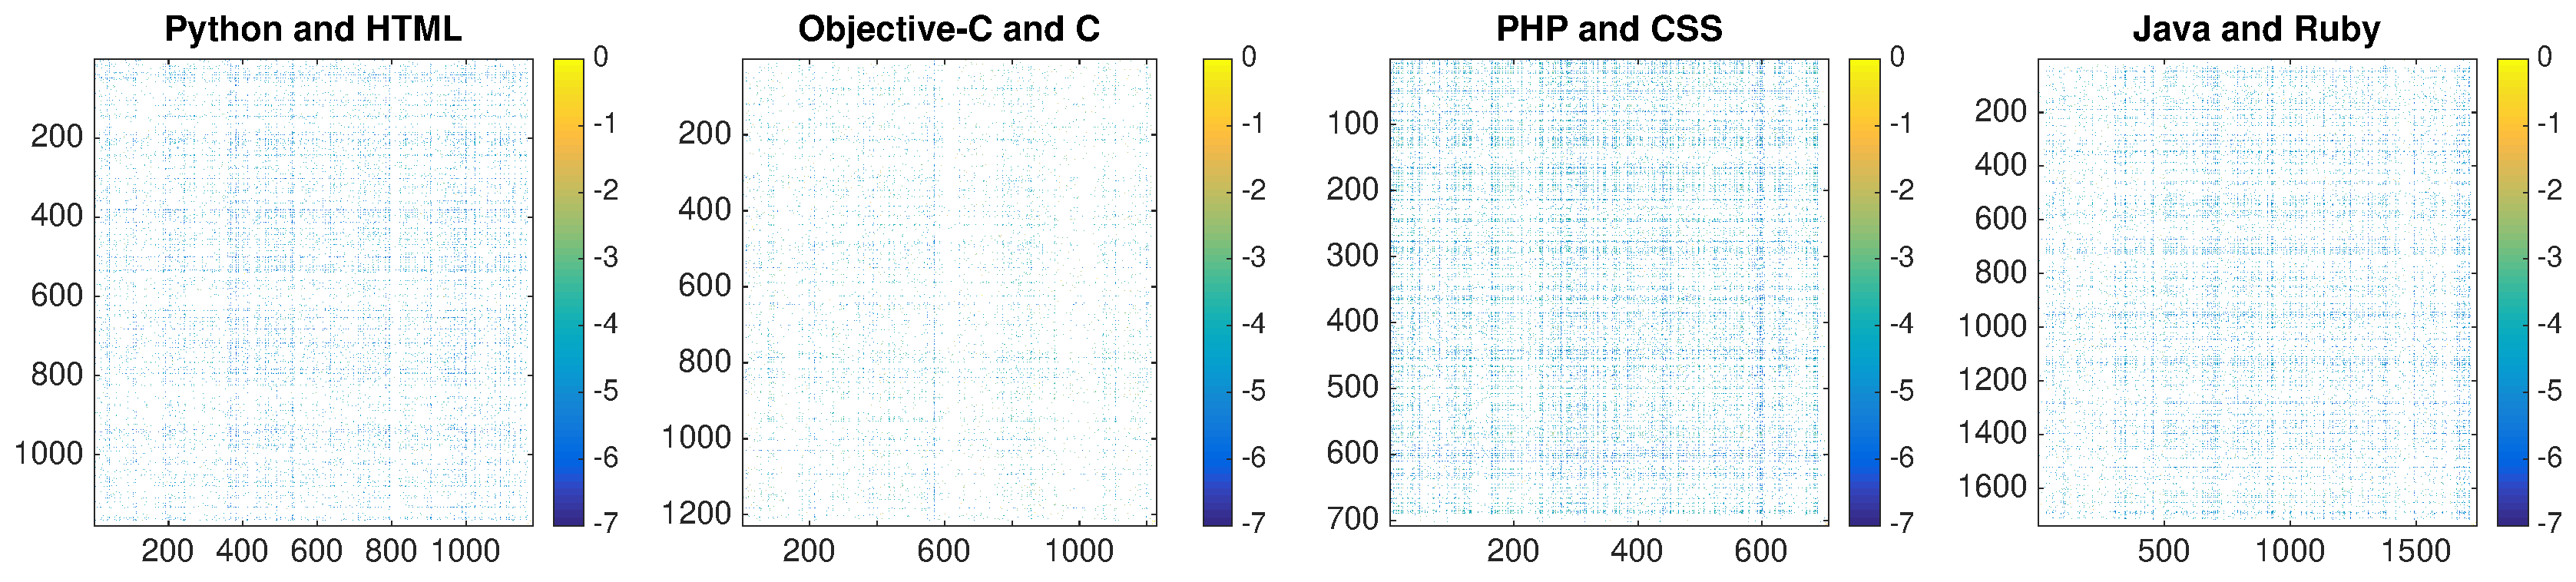
\includegraphics[width = 6 in]{figure/con_Jaccard_greedy.eps}}
	\subcaptionbox{Dot product + idf}{
		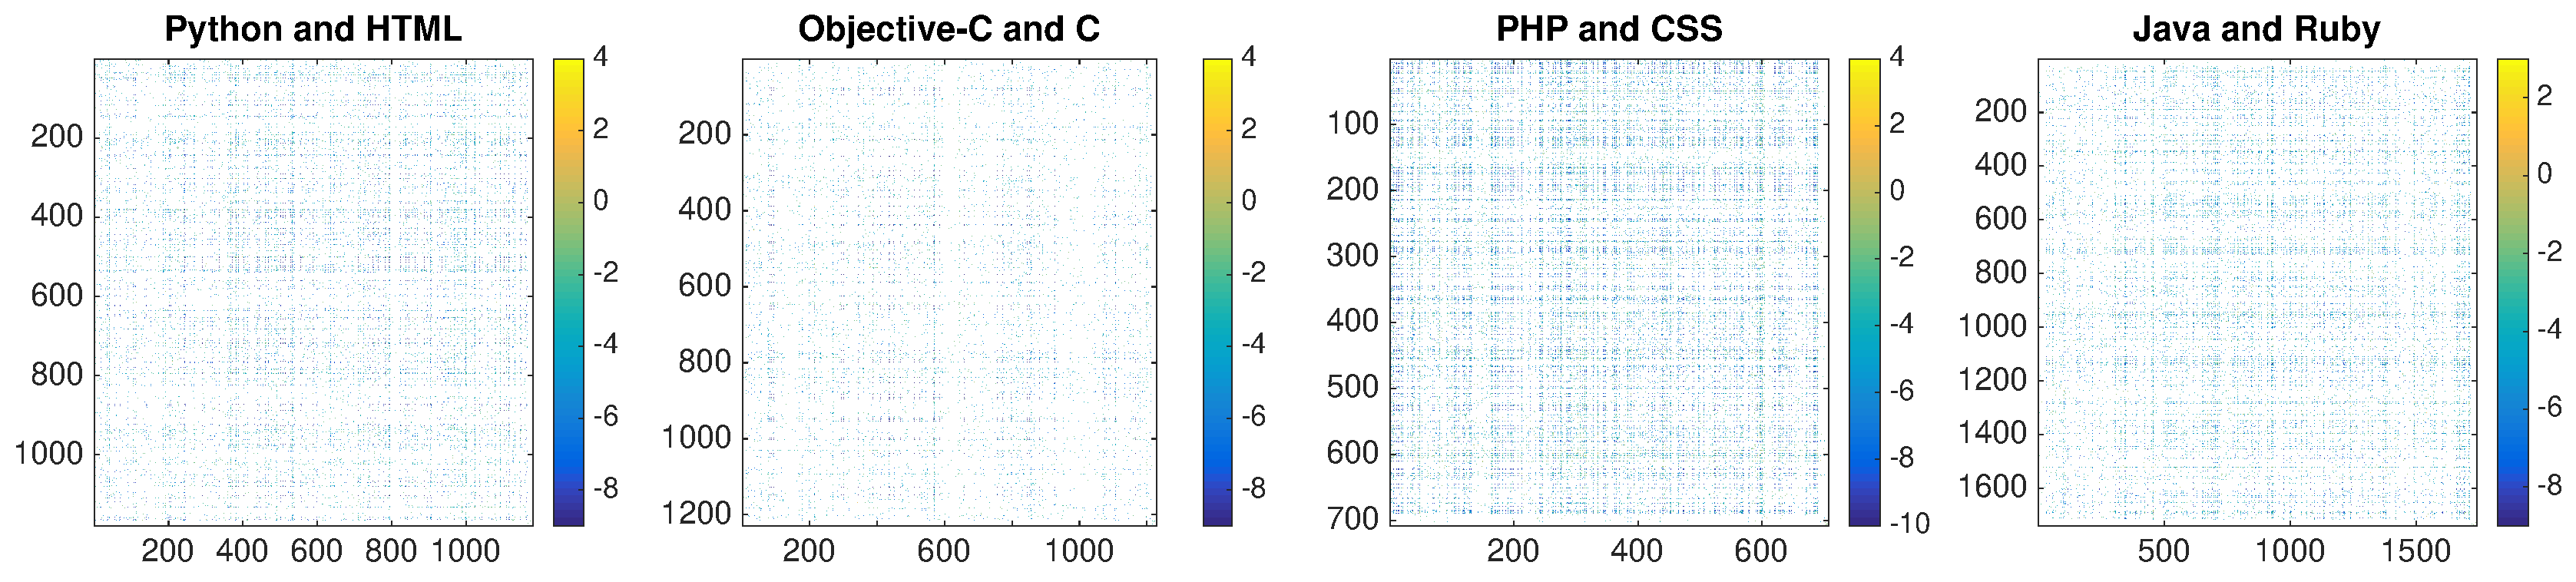
\includegraphics[width = 6 in]{figure/con_idf_intersection_greedy.eps}}
	\subcaptionbox{Cosine + idf}{
		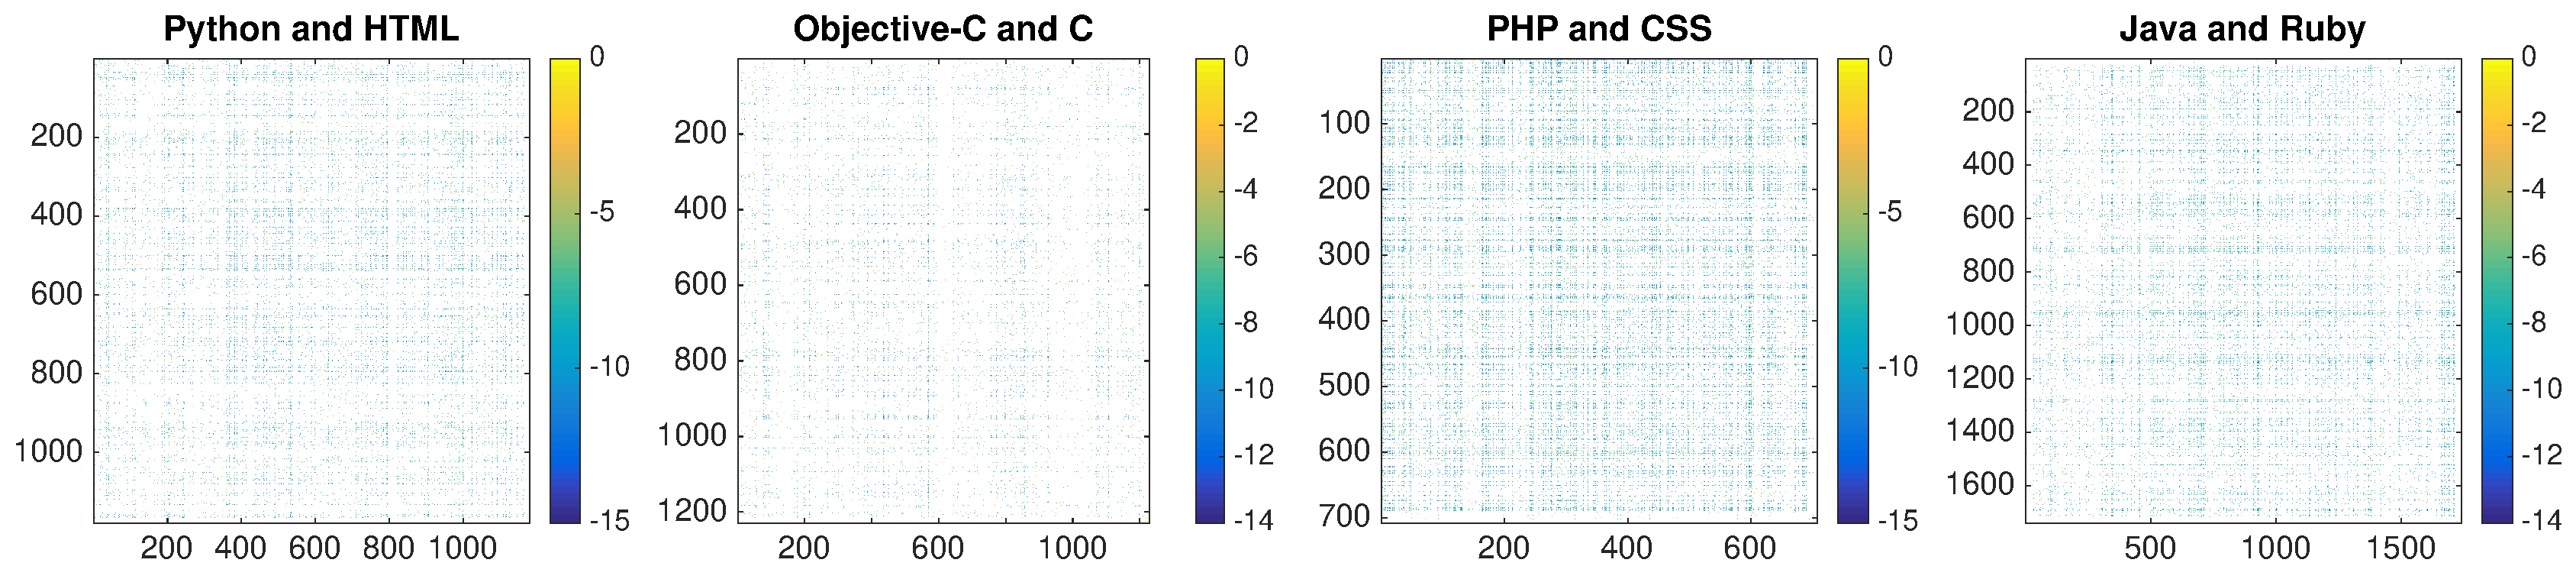
\includegraphics[width = 6 in]{figure/con_idf_cosine_greedy.eps}}
	\caption{Clustering result by greedy algorithm of subnetworks transformed from repository-contributor subnetworks}
	\label{fig:clustering result by greedy algorithm of repository-contributor network}
\end{figure*}

\begin{figure*}
	\centering
	\subcaptionbox{Dot product}{
		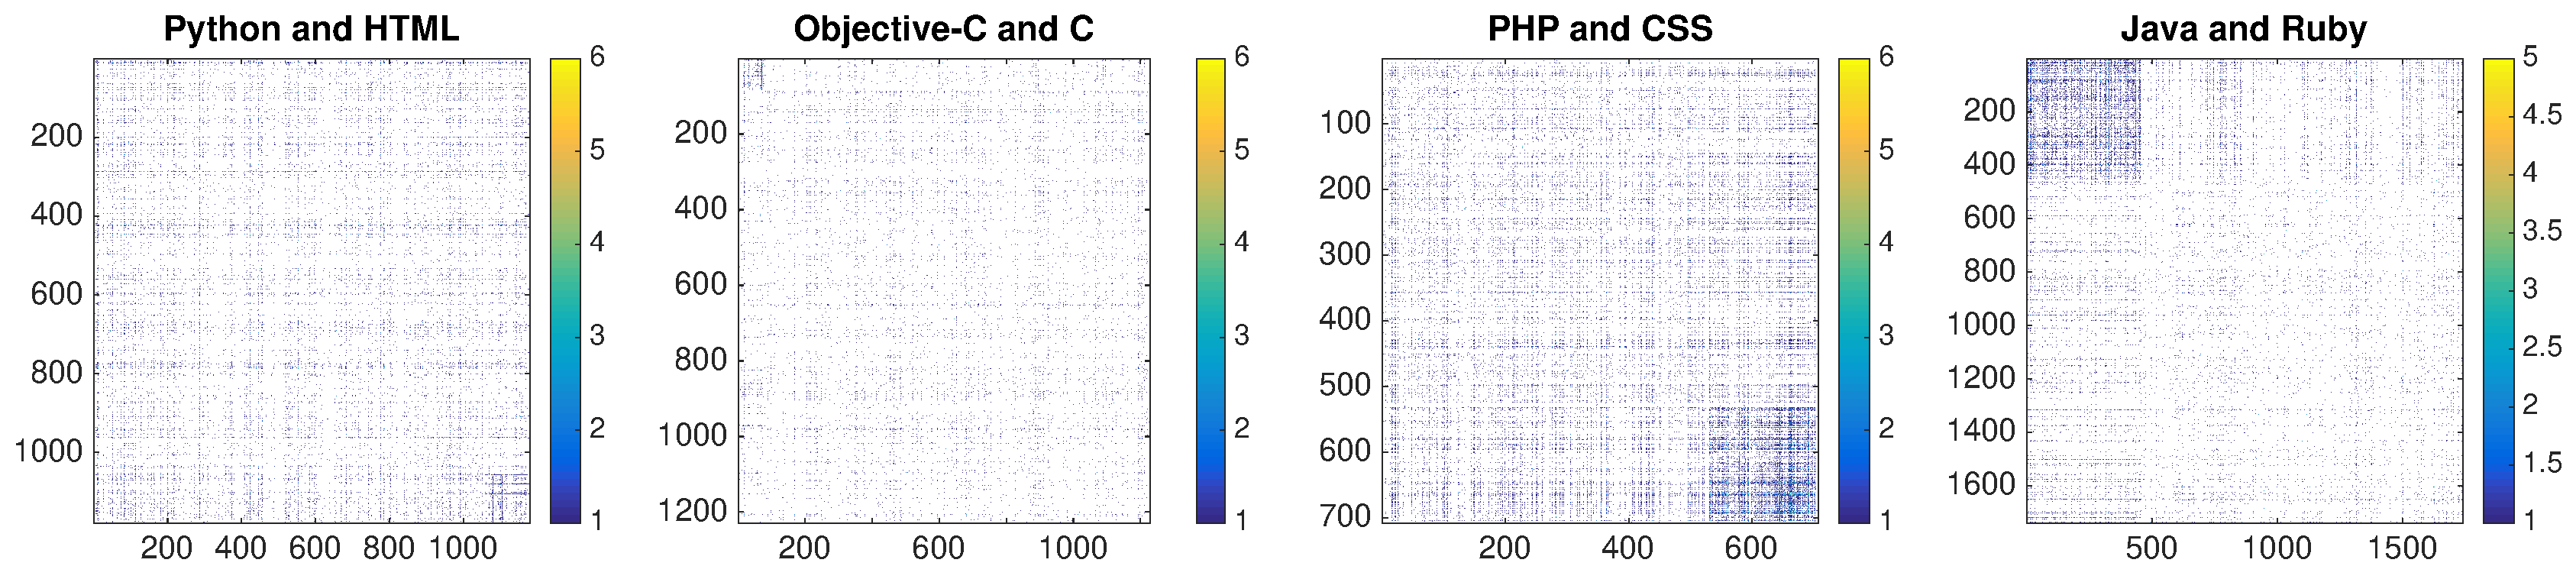
\includegraphics[width = 6 in]{figure/con_intersection_spectral.eps}}
	\subcaptionbox{Cosine}{
		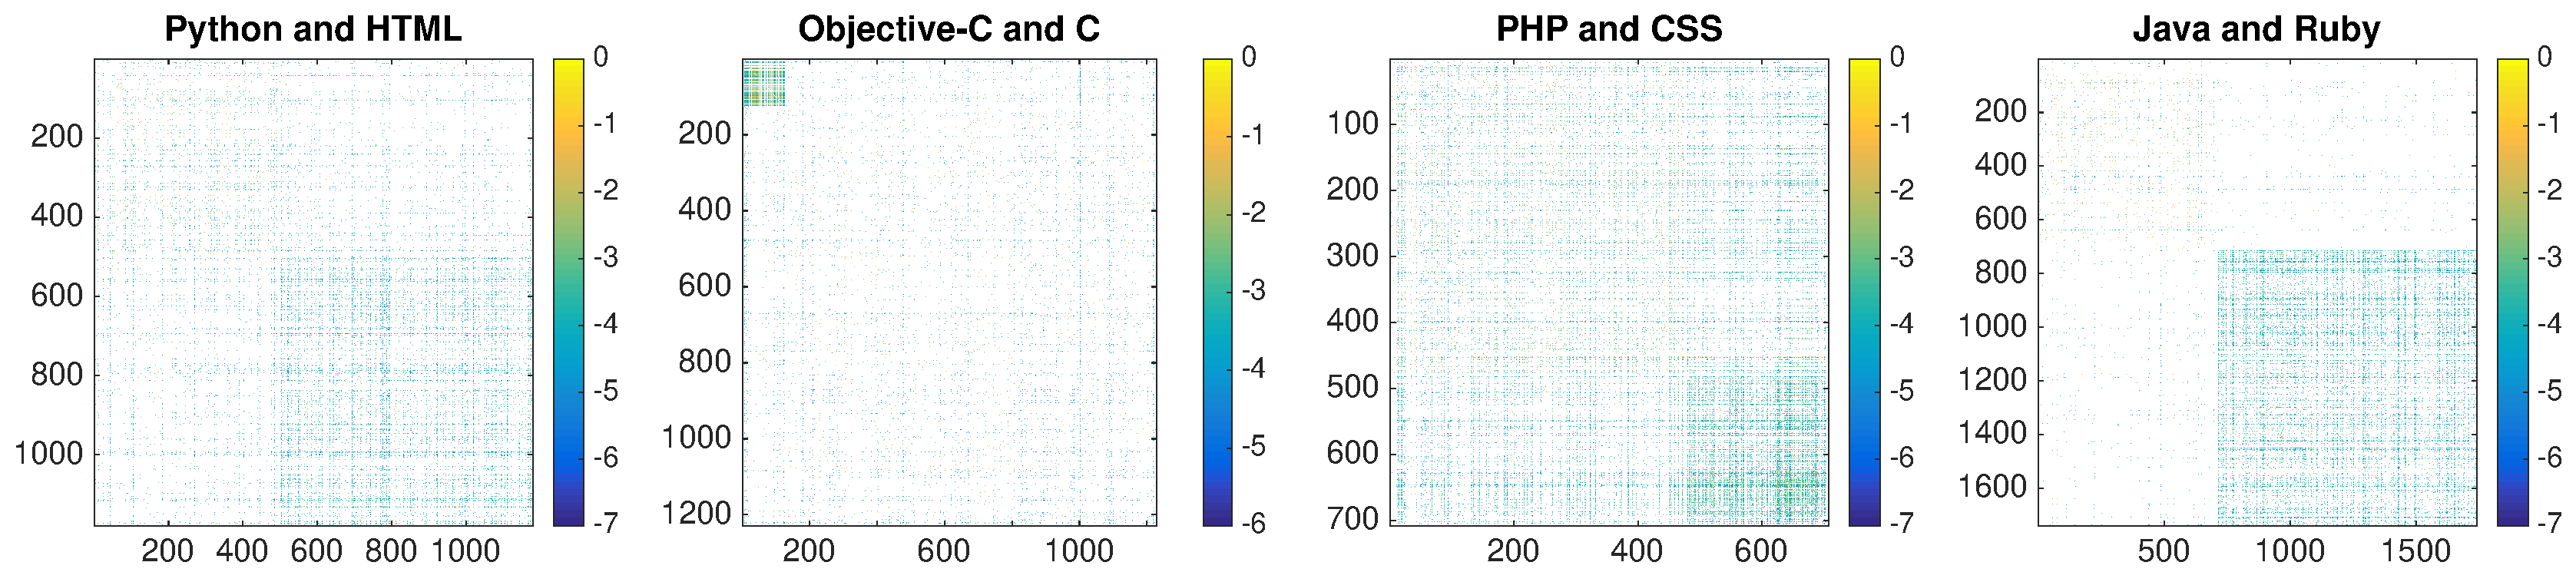
\includegraphics[width = 6 in]{figure/con_cosine_spectral.eps}}
	\subcaptionbox{Jaccard}{
		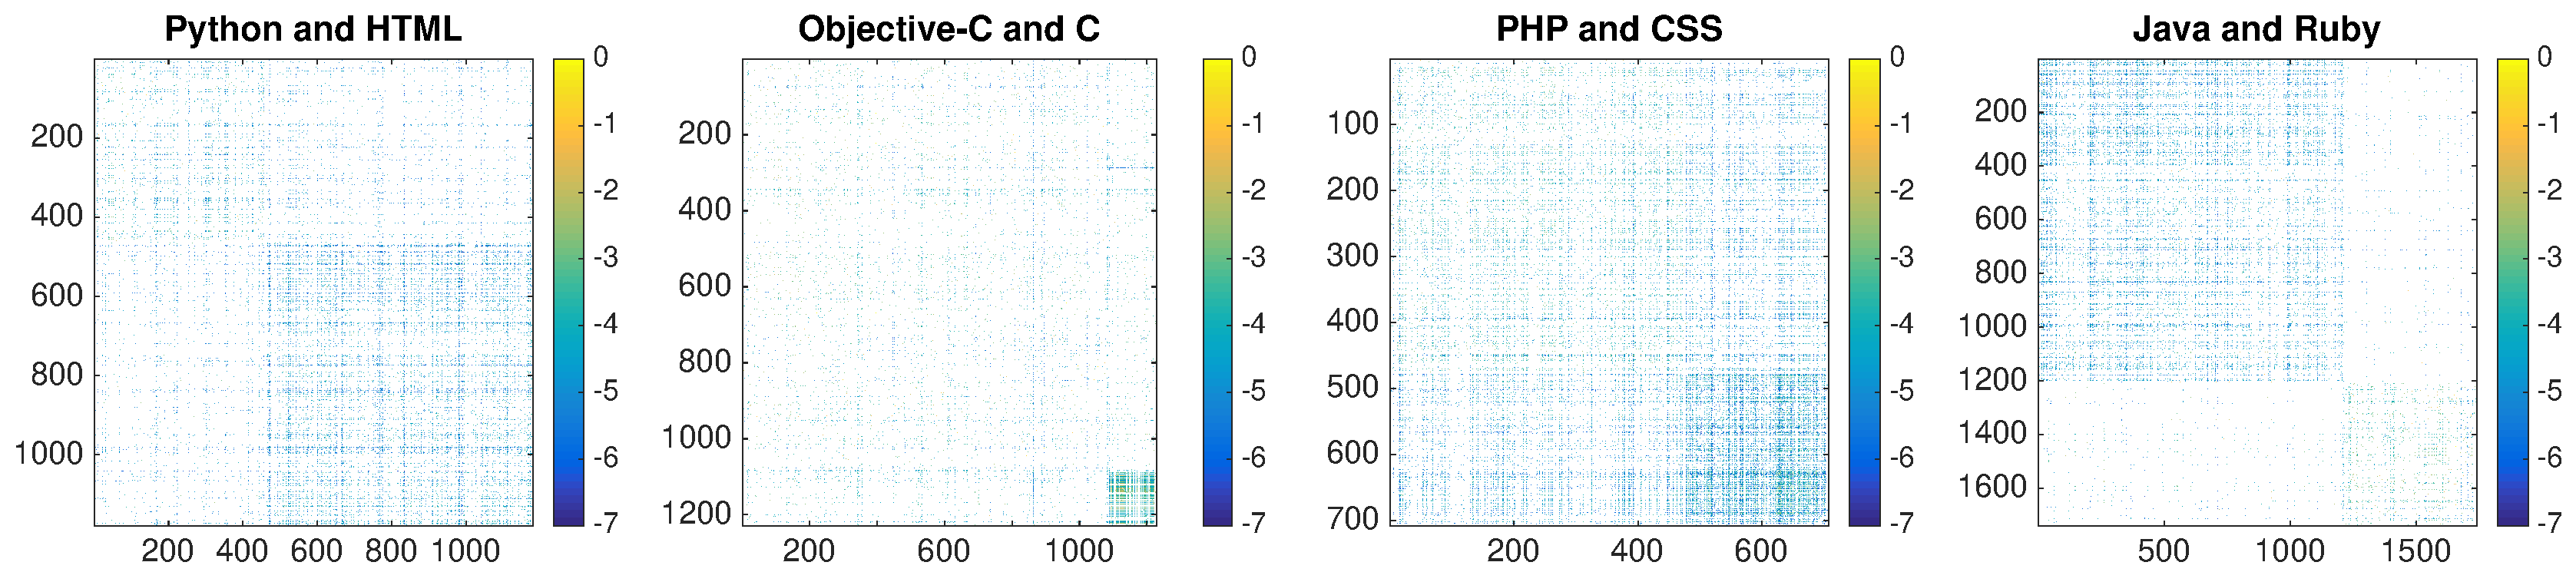
\includegraphics[width = 6 in]{figure/con_Jaccard_spectral.eps}}
	\subcaptionbox{Dot product + idf}{
		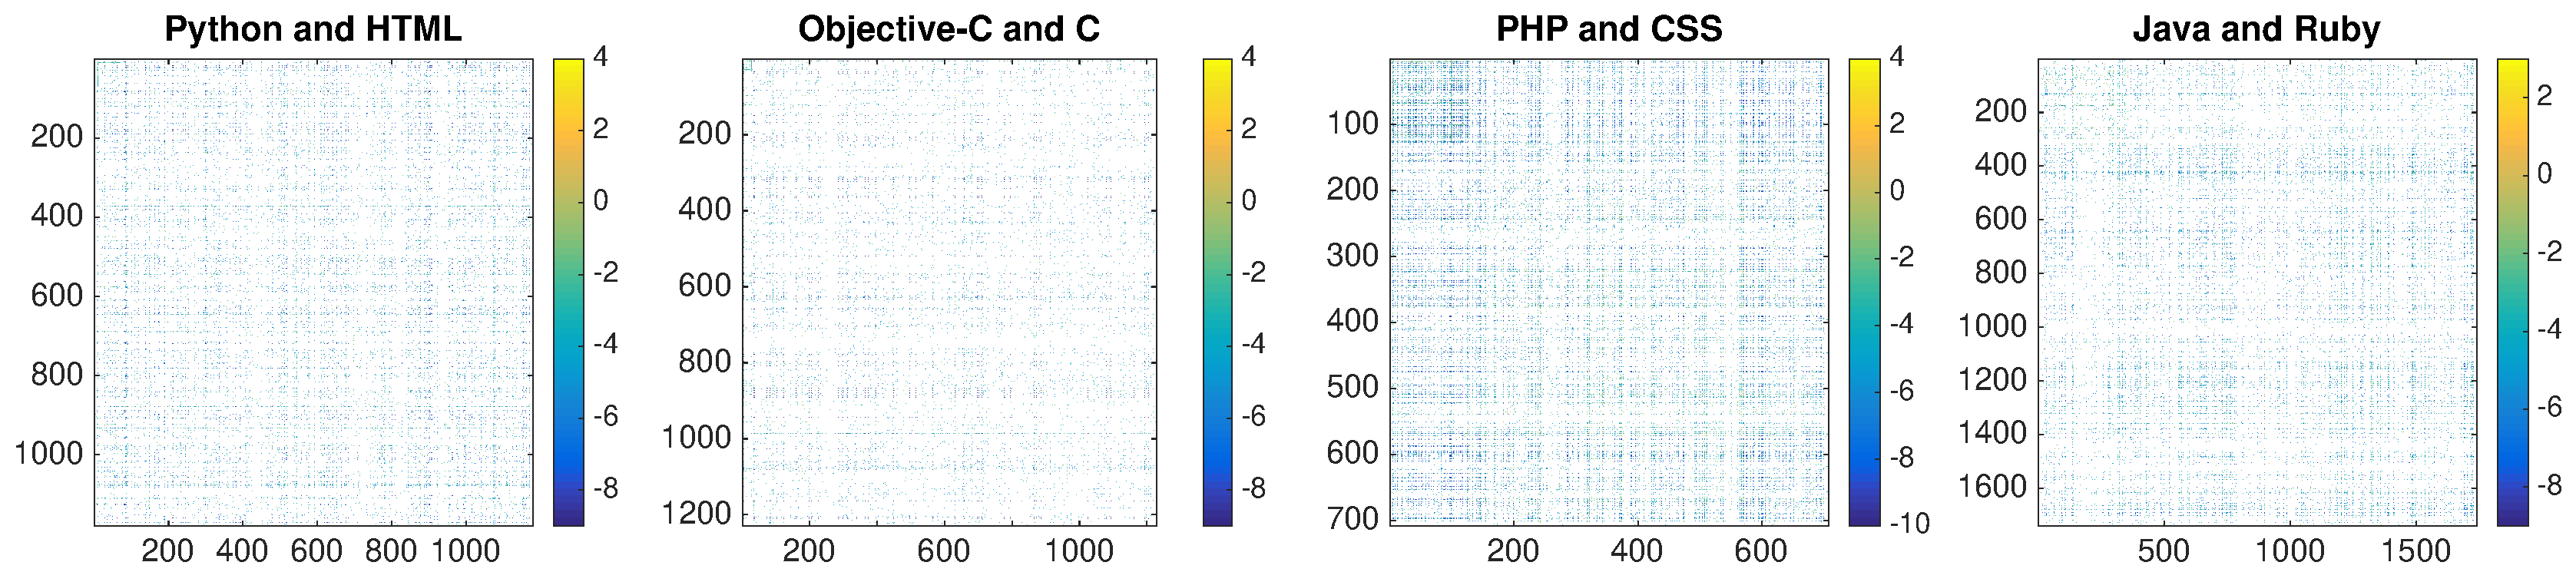
\includegraphics[width = 6 in]{figure/con_idf_intersection_spectral.eps}}
	\subcaptionbox{Cosine + idf}{
		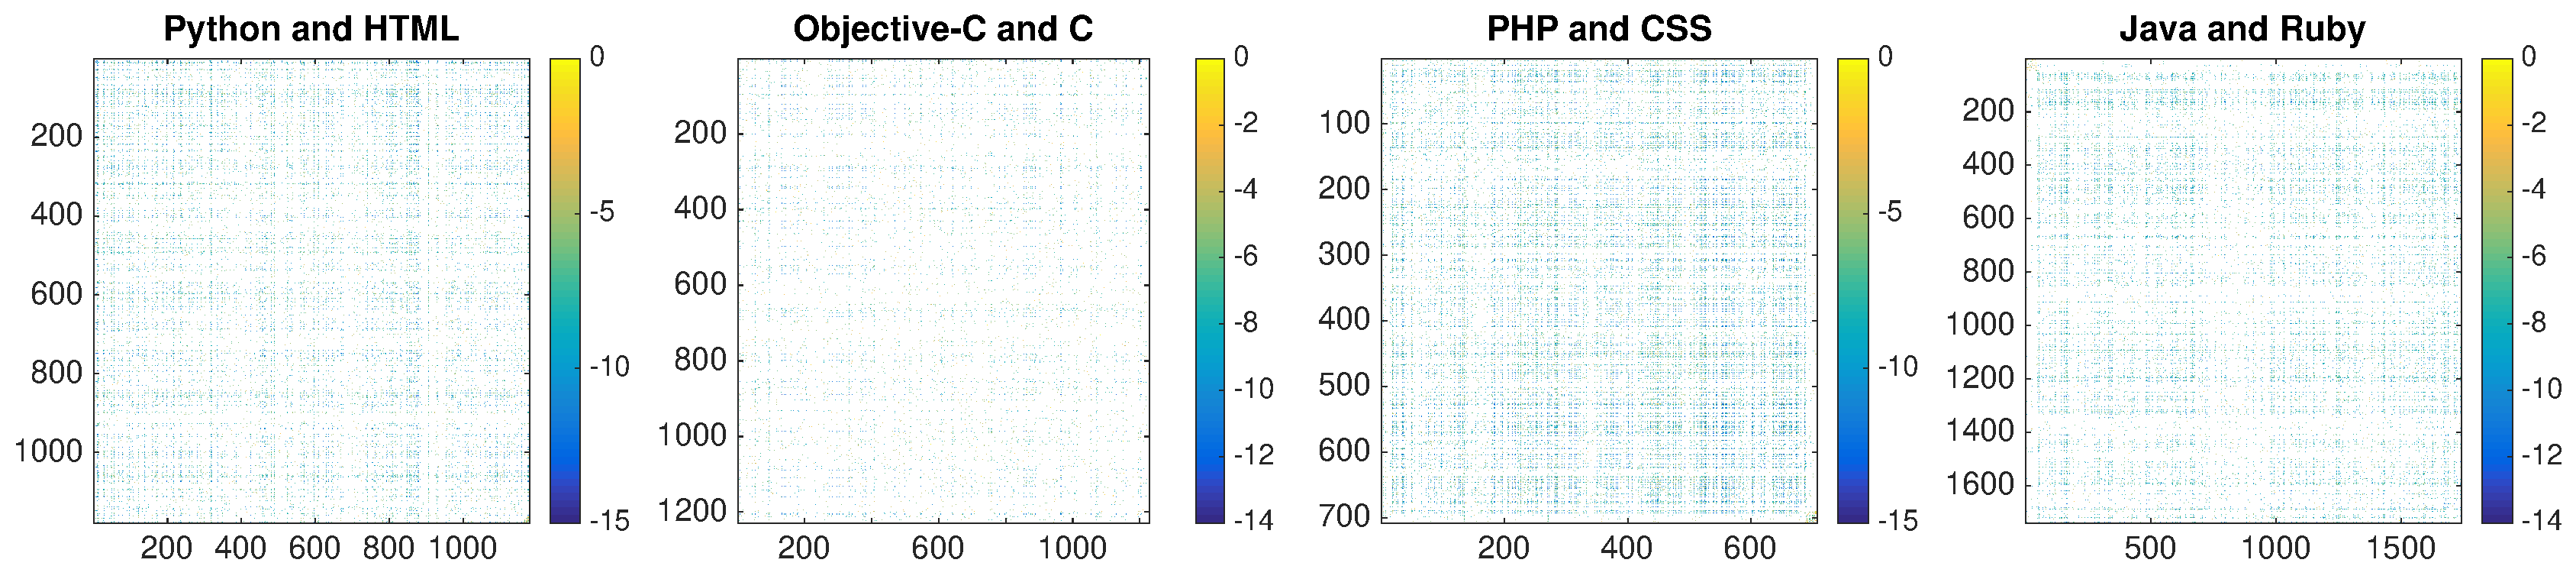
\includegraphics[width = 6 in]{figure/con_idf_cosine_spectral.eps}}
	\caption{Clustering result by spectral algorithm of subnetworks transformed from repository-contributor subnetworks}
	\label{fig:clustering result by spectral algorithm of repository-contributor network}
\end{figure*}

%\begin{table*}
%	\begin{tabular}{c|c|cc|cc} \toprule
%		\multirow{2}{*}{Dataset}&\multirow{2}{*}{Transform approach} & \multicolumn{2}{c}{Greedy Algorithm} &  \multicolumn{2}{|c}{Spectral Algorithm} \\ \cline{3-6}
%		& & F-measure & Rand Index & F-measure & Rand Index \\ \hline
%		\multirow{5}*{\minitab[c]{Python \\ and \\ HTML}}&\multirow{5}{*}{}  Dot product & 0.7598 & 0.6042  & 0.7245 & 0.5524\\ 
%		&Cosine      & 0.7598 & 0.6042 & 0.7278 & 0.5696 \\ 
%		&Jaccard     & 0.7598 & 0.6042  & 0.7284 & 0.5715\\ 
%		&Dot product + idf & 0.7598 & 0.6042  & 0.7396 & 0.5715 \\ 
%		&Cosine + idf    & 0.7598 & 0.6042  & \textbf{0.7584} & \textbf{0.6003} \\  \hline
%		
%		\multirow{5}*{\minitab[c]{Objective-C \\ and \\ C}} & \multirow{5}{*}{}  Dot product & 0.7479 & 0.5827  & 0.7436 & \textbf{0.6323} \\ 
%		&Cosine     & 0.7479 & 0.5827  & 0.7071 & 0.5280 \\ 
%		&Jaccard     & 0.7479 & 0.5827  & 0.7061 & 0.5261 \\ 
%		&Dot product + idf & 0.7479 & 0.5827  & 0.7490 & 0.6099 \\ 
%		&Cosine + idf    & 0.7479 & 0.5827  & \textbf{0.7510} & 0.5930 \\ \hline
%		
%		\multirow{5}*{\minitab[c]{PHP \\ and \\ CSS}}  & \multirow{5}{*}{}  Dot product & 0.7247 & 0.5361  & 0.6381 & 0.5034 \\ 
%		&Cosine      & 0.7247 & 0.5361  & 0.6088 & 0.5118 \\ 
%		&Jaccard     & 0.7247 & 0.5361  & 0.607 & 0.5123 \\ 
%		&Dot product + idf & 0.7247 & 0.5361  & 0.6641 & 0.4993 \\ 
%		&Cosine + idf    & 0.7247 & 0.5361  & \textbf{0.7209} & \textbf{0.5417} \\ \hline
%		
%		\multirow{5}*{\minitab[c]{Java \\ and \\ Ruby}} & \multirow{5}{*}{}  Dot product & 0.6891 & 0.5000  & 0.7503 & 0.6158 \\ 
%		&Cosine      & 0.6891 & 0.5000 & \textbf{0.9304} & \textbf{0.8329} \\ 
%		&Jaccard     & 0.6891 & 0.5000 & 0.8074 & 0.6784 \\ 
%		&Dot product + idf & 0.6891 & 0.5000  & 0.6410 & 0.4997 \\ 
%		&Cosine + idf    & 0.6891 & 0.5000  & 0.6838 & 0.5016 \\  \bottomrule
%	\end{tabular}
%	\caption{Evaluation result of subnetworks transformed from repository-contributor subnetworks}
%	\label{tab:evaluation result of repository-contributor network}
%\end{table*}

\begin{table*}
	\centering
	\begin{tabular}{c|c|P{1cm}P{1cm}P{1cm}|P{1cm}P{1cm}P{1cm}} \toprule
		\multirow{2}{*}{Dataset}&\multirow{2}*{\minitab[c]{Transform \\ approach}} & \multicolumn{3}{c}{Greedy Algorithm} &  \multicolumn{3}{|c}{Spectral Algorithm} \\ \cline{3-8}
		& & M & F & RI & M & F & RI \\ \hline
		\multirow{5}*{\minitab[c]{Python \\ and \\ HTML}}&\multirow{5}{*}{}  Dot product & 0.0002 & 0.7598 & 0.6042  &0.0572& 0.7245 & 0.5524\\ 
		&Cosine      &0.0049& 0.7598 & 0.6042 & 0.2608& 0.7278 & 0.5696 \\ 
		&Jaccard     & 0.0076&0.7598 & 0.6042  &0.2750& 0.7284 & 0.5715\\ 
		&Dot product + idf &0.0012& 0.7598 & 0.6042  & 0.0765 & 0.7396 & 0.5715 \\ 
		&Cosine + idf    & 0.0321 &0.7598 & 0.6042  & 0.0371& \textbf{0.7584} & \textbf{0.6003} \\  \hline
		
		\multirow{5}*{\minitab[c]{Objective-C \\ and \\ C}} & \multirow{5}{*}{}  Dot product &0.0007& 0.7479 & 0.5827 &0.1787 & 0.7436 & \textbf{0.6323} \\ 
		&Cosine     & 0.0127& 0.7479 & 0.5827  & 0.2859&0.7071 & 0.5280 \\ 
		&Jaccard     & 0.0249& 0.7479 & 0.5827  & 0.2890 & 0.7061 & 0.5261 \\ 
		&Dot product + idf & 0.0017 &0.7479 & 0.5827 &0.1501  & 0.7490 & 0.6099 \\ 
		&Cosine + idf    & 0.0742&0.7479 & 0.5827 &0.0737  & \textbf{0.7510} & 0.5930 \\ \hline
		
		\multirow{5}*{\minitab[c]{PHP \\ and \\ CSS}}  & \multirow{5}{*}{}  Dot product &0.0001 &0.7247 & 0.5361  &0.2311 &0.6381 & 0.5034 \\ 
		&Cosine      &0.0022 &0.7247 & 0.5361  &0.2345 &0.6088 & 0.5118 \\ 
		&Jaccard     &0.0022 &0.7247 & 0.5361  &0.2388 &0.607 & 0.5123 \\ 
		&Dot product + idf &0.0007 &0.7247 & 0.5361  &0.1765 &0.6641 & 0.4993 \\ 
		&Cosine + idf    &0.0181 &0.7247 & 0.5361  &0.0514 &\textbf{0.7209} & \textbf{0.5417} \\ \hline
		
		\multirow{5}*{\minitab[c]{Java \\ and \\ Ruby}} & \multirow{5}{*}{}  Dot product &0.0002 &0.6891 & 0.5000  &0.1601 &0.7503 & 0.6158 \\ 
		&Cosine      &0.0051 &0.6891 & 0.5000 &0.3557 &\textbf{0.9304} & \textbf{0.8329} \\ 
		&Jaccard     &0.0089 &0.6891 & 0.5000 &0.3125 &0.8074 & 0.6784 \\ 
		&Dot product + idf &0.0013 &0.6891 & 0.5000  &0.1279 &0.6410 & 0.4997 \\ 
		&Cosine + idf    &0.0329 &0.6891 & 0.5000  &0.0830 &0.6838 & 0.5016 \\  \bottomrule
	\end{tabular}
	\caption{Evaluation result of subnetworks transformed from repository-contributor subnetworks, M: Modularity, F: F-measure, RI:Rand Index}
	\label{tab:evaluation result of repository-contributor network}
\end{table*}
Then we clustered repository networks, obtained from the repository-stargazer network. Figure \ref{fig:clustering result by greedy algorithm of repository-stargazer network} and Figure \ref{fig:clustering result by spectral algorithm of repository-stargazer network}  separately display the clustering results for both clustering algorithms. Unlike the network transformed from the repository-contributor network, this time, we can clearly differentiate two categories of repositories from all the figures, no matter which the weighting schemes or the clustering algorithms we applied, although in some figures there is only one distinct community. We also noticed that  in most of the figures, the connection between the repositories in the same community is tighter than the repository in different communities. In addition, just considering the number of repositories of each community, the result of dot product is more like the ground truth than the other two weighting schemes. If we apply the inverse document frequency, both dot product and cosine similarity perform better than the original ones. Table \ref{tab:evaluation result of repository-stargazer network} displays the value of modularity and the evaluation measure values of community structures detected by the two clustering algorithms on these subnetworks. For the modularity, we found that the inverse document frequency increases the value of both dot product and cosine similarity for both clustering algorithms. In addition, in PHP and CSS dataset and Java and Ruby dataset, cosine similarity and Jaccard similarity performs better and dot product. But in Objective-C and C dataset, dot product receives the highest value of modularity for both algorithms. In Python and HTML dataset, dot product and Jaccard similarity separately obtain higher value than the other two weighting schemes for greedy algorithm and spectral algorithm. When we cluster the subnetworks by the greedy algorithm, the combination of dot product and inverse document frequency performs better than the other weighting schemes and it gets the highest value of both evaluation measures on Python and HTML dataset, Objective-C and C dataset and Java and Ruby dataset. While on the PHP and CSS dataset, dot product obtains the best result value of F-measures and rand index, separately 0.8714 and 0.7740. However, for the spectral algorithm, the combination of dot product and inverse document gets the highest value for both evaluation measures on all four datasets. 

\begin{figure*}
	\centering
	\subcaptionbox{Dot product}{
		\includegraphics[width = 6 in]{figure/star_intersection_greedy.eps}}
	\subcaptionbox{Cosine}{
		\includegraphics[width = 6 in]{figure/star_cosine_greedy.eps}}
	\subcaptionbox{Jaccard}{
		\includegraphics[width = 6 in]{figure/star_Jaccard_greedy.eps}}
	\subcaptionbox{Dot product + idf}{
		\includegraphics[width = 6 in]{figure/star_idf_intersection_greedy.eps}}
	\subcaptionbox{Cosine + idf}{
		\includegraphics[width = 6 in]{figure/star_idf_cosine_greedy.eps}}
	\caption{Clustering result by greedy algorithm of subnetworks transformed from repository-stargazer subnetworks}
	\label{fig:clustering result by greedy algorithm of repository-stargazer network}
\end{figure*}

\begin{figure*}
	\centering
	\subcaptionbox{Dot product}{
		\includegraphics[width = 6 in]{figure/star_intersection_spectral.eps}}
	\subcaptionbox{Cosine}{
		\includegraphics[width = 6 in]{figure/star_cosine_spectral.eps}}
	\subcaptionbox{Jaccard}{
		\includegraphics[width = 6 in]{figure/star_Jaccard_spectral.eps}}
	\subcaptionbox{Dot product + idf}{
		\includegraphics[width = 6 in]{figure/star_idf_intersection_spectral.eps}}
	\subcaptionbox{Cosine + idf}{
		\includegraphics[width = 6 in]{figure/star_idf_cosine_spectral.eps}}
	\caption{Clustering result by spectral algorithm of subnetworks transformed from repository-stargazer subnetworks}
	\label{fig:clustering result by spectral algorithm of repository-stargazer network}
\end{figure*}

%\begin{table*}
%	\begin{tabular}{c|c|cc|cc} \toprule
%		\multirow{2}{*}{Dataset}&\multirow{2}{*}{Transform approach} & \multicolumn{2}{c}{Greedy Algorithm} &  \multicolumn{2}{|c}{Spectral Algorithm} \\ \cline{3-6}
%		& & F-measure & Rand Index & F-measure & Rand Index \\ \hline
%		\multirow{5}*{\minitab[c]{Python \\ and \\ HTML}}&\multirow{5}{*}{}  Dot product & 0.7245 & 0.5884  & 0.8278 & 0.7043 \\ 
%		&Cosine     & 0.7809 & 0.6455  & 0.6983 & 0.5678 \\ 
%		&Jaccard     & 0.7902 & 0.6559  & 0.6943 & 0.5649 \\ 
%		&Dot product + idf & \textbf{0.8743} & \textbf{0.7800} & \textbf{0.8658} & \textbf{0.7649} \\ 
%		&Cosine + idf    & 0.6681 & 0.5474  & 0.7239 & 0.5878 \\  \hline
%		
%		\multirow{5}*{\minitab[c]{Objective-C \\ and \\ C}}  & \multirow{5}{*}{}  Dot product & 0.9040 & 0.8219  & 0.8623 & 0.7545 \\ 
%		&Cosine      & 0.7593 & 0.6238  & 0.7585 & 0.623 \\ 
%		&Jaccard     & 0.7196 & 0.5871  & 0.6699 & 0.5514 \\ 
%		&Dot product + idf & \textbf{0.9189} & \textbf{0.8478} & \textbf{0.9432} & \textbf{0.8919} \\ 
%		&Cosine + idf    & 0.9048 & 0.8231  & 0.8645 & 0.7577 \\ \hline
%		
%		\multirow{5}*{\minitab[c]{PHP \\ and \\ CSS}}  & \multirow{5}{*}{}  Dot product & \textbf{0.8714} & \textbf{0.7740}  & 0.8829 & 0.7914 \\ 
%		&Cosine      & 0.8508 & 0.7444   & 0.8573 & 0.7535 \\ 
%		&Jaccard     & 0.8496 & 0.7426  & 0.8521 & 0.7462\\ 
%		&Dot product + idf & 0.8339 & 0.7216  & \textbf{0.9045} & \textbf{0.8258} \\ 
%		&Cosine + idf    & 0.8008 & 0.6808  & 0.8274 & 0.7131 \\  \hline
%		
%		\multirow{5}*{\minitab[c]{Java \\ and \\ Ruby}} &  Dot product & 0.8677 & 0.7724  & 0.9090 & 0.8350 \\ 
%		&Cosine      & 0.8694 & 0.7749  & 0.8935 & 0.8106 \\ 
%		&Jaccard     & 0.8688 & 0.7740  & 0.8868 & 0.8004 \\ 
%		&Dot product + idf  & \textbf{0.9756} & \textbf{0.9523}  & \textbf{0.9582} & \textbf{0.9198} \\ 
%		&Cosine + idf    & 0.9723 & 0.9461  & 0.9391 & 0.8857 \\  \bottomrule
%	\end{tabular}
%	\caption{Evaluation result of subnetworks transformed from repository-stargazer subnetworks}
%	\label{tab:evaluation result of repository-stargazer network}
%\end{table*}

\begin{table*}
	\centering
	\begin{tabular}{c|c|P{1.1cm}P{1.1cm}P{1.1cm}|P{1.1cm}P{1.1cm}P{1.1cm}} \toprule
		\multirow{2}{*}{Dataset}&\multirow{2}*{\minitab[c]{Transform \\ approach}} & \multicolumn{3}{c}{Greedy Algorithm} &  \multicolumn{3}{|c}{Spectral Algorithm} \\ \cline{3-8}
		& & M & F & RI & M & F & RI \\ \hline
		\multirow{5}*{\minitab[c]{Python \\ and \\ HTML}}&\multirow{5}{*}{}  Dot product &0.1185 &0.7245 & 0.5884  &0.1169 &0.8278 & 0.7043 \\ 
		&Cosine     &0.0969 &0.7809 & 0.6455  &0.1203 &0.6983 & 0.5678 \\ 
		&Jaccard     &0.1055 &0.7902 & 0.6559  &0.1229 &0.6943 & 0.5649 \\ 
		&Dot product + idf &0.2020 &\textbf{0.8743} & \textbf{0.7800} &0.2029 &\textbf{0.8658} & \textbf{0.7649} \\ 
		&Cosine + idf    &0.2215 &0.6681 & 0.5474  &0.2198 &0.7239 & 0.5878 \\  \hline
		
		\multirow{5}*{\minitab[c]{Objective-C \\ and \\ C}}  & \multirow{5}{*}{}  Dot product &0.0974 &0.9040 & 0.8219  &0.0965 &0.8623 & 0.7545 \\ 
		&Cosine      &0.0940 &0.7593 & 0.6238  &0.0936 &0.7585 & 0.623 \\ 
		&Jaccard     &0.0937 &0.7196 & 0.5871  &0.0914 &0.6699 & 0.5514 \\ 
		&Dot product + idf &0.3499 &\textbf{0.9189} & \textbf{0.8478} &0.3394 &\textbf{0.9432} & \textbf{0.8919} \\ 
		&Cosine + idf    &0.2369 &0.9048 & 0.8231  &0.2384 &0.8645 & 0.7577 \\ \hline
		
		\multirow{5}*{\minitab[c]{PHP \\ and \\ CSS}}  & \multirow{5}{*}{}  Dot product &0.1695 &\textbf{0.8714} & \textbf{0.7740}  &0.1690 &0.8829 & 0.7914 \\ 
		&Cosine      & 0.1722 &0.8508 & 0.7444   &0.1721 &0.8573 & 0.7535 \\ 
		&Jaccard     &0.1766 &0.8496 & 0.7426  &0.1763 &0.8521 & 0.7462\\ 
		&Dot product + idf &0.2770 &0.8339 & 0.7216  &0.2333 &\textbf{0.9045} & \textbf{0.8258} \\ 
		&Cosine + idf    &0.2261 &0.8008 & 0.6808  &0.2822 &0.8274 & 0.7131 \\  \hline
		
		\multirow{5}*{\minitab[c]{Java \\ and \\ Ruby}} &  Dot product &0.3999 &0.8677 & 0.7724  &0.4000 &0.9090 & 0.8350 \\ 
		&Cosine      &0.4079 &0.8694 & 0.7749  &0.4073& 0.8935 & 0.8106 \\ 
		&Jaccard     &0.4108 &0.8688 & 0.7740  &0.4100 &0.8868 & 0.8004 \\ 
		&Dot product + idf  &0.3206 &\textbf{0.9756} & \textbf{0.9523}  &0.3166 &\textbf{0.9582} & \textbf{0.9198} \\ 
		&Cosine + idf    &0.4037 &0.9723 & 0.9461  &0.4066 &0.9391 & 0.8857 \\  \bottomrule
	\end{tabular}
	\caption{Evaluation result of subnetworks transformed from repository-stargazer subnetworks, M: Modularity, F: F-measure, RI:Rand Index}
	\label{tab:evaluation result of repository-stargazer network}
\end{table*}

\subsection{Distribution of Weighting Schemes}
From the experiments, we fount that Dot product is best weighting schemes in most case and inverse document frequency greatly improve the performance of both dot product and cosine similarity. To explain this phenomenon, we firstly plotted the distribution of all weighting schemes. Figure \ref{fig:weight degree distribution of repository-contributor} and Figure \ref{fig:weight degree distribution of repository-stargazer} separately plot the distribution of weighting schemes of repository subnetworks obtained by the transformation of repository-contributor subnetworks and repository-stargazer subnetworks. From Figure \ref{fig:weight degree distribution of repository-contributor}, we noticed that for each weighting schemes, the distribution of all four subnetworks is shown the same trend. For both dot product and the combination of cosine similarity and inverse document frequency, the distribution follows a power law distribution. Without applying the inverse document frequency, the distribution of cosine similarity increases at first and reach the peak around 0.01. Then it begins to decrease and follows a power law distribution. However, the distribution of Jaccard similarity is strange. At the beginning, it climbs to the top when the value of Jaccard similarity is around 0.005 and then begins to drop. But during the process of reducing,with the increase of Jaccard similarity value, there is a gap for the count. In addition, this phenomenon is also shown in the distribution of the combination of dot product and inverse document frequency, although it follows a power law distribution. Comparing the three weighting schemes, we found that for all the four datasets, the count of dot product, which is equal to 1, is the largest one, but the large count of cosine similarity and Jaccard similarity obtains the largest count at the medium value. If we apply the inverse document frequency, we noticed although there is a large number weight gets small value, there is also a lot of weight get higher values. However, the distribution of cosine similarity follows a power law distribution. From the result we found that the combination of cosine similarity and inverse document frequency achieves the best performance, so I think that if the distribution follows a power law distribution, the network may be clustered more like the original one. 

For the repository subnetworks transformed from the repository-stargazer subnetworks, the distribution of dot product, the combination of dot product and inverse document frequency and the combination of cosine similarity and inverse document frequency follows a power law distribution. While for the other two weighting schemes, except the increase at the start, they also follow a power law distribution. Besides we also noticed that the distribution of Objective-C and C dataset transformed by cosine similarity and Jaccard similarity has a phase that the count of value remains constant.  Comparing the distribution of dot product, cosine similarity, and Jaccard similarity, we found that there is a lot of weight gets small values of dot product, but the number of small weight of cosine similarity and Jaccard similarity is far less than dot product. Most of the weight of cosine similarity and Jaccard similarity gets medium value. This may cause the performance of cosine similarity and Jaccard similarity worse than dot product. However, when we apply the inverse document frequency, cosine similarity shows the same distribution as dot product, and this explains why the inverse document frequency significantly improves the value of evaluation measures. In addition, we found that after the inverse document frequency, the distribution of dot product is tighter than the original one and it also performs better. 
\begin{figure*}
	\centering
	\subcaptionbox{Dot product}{
		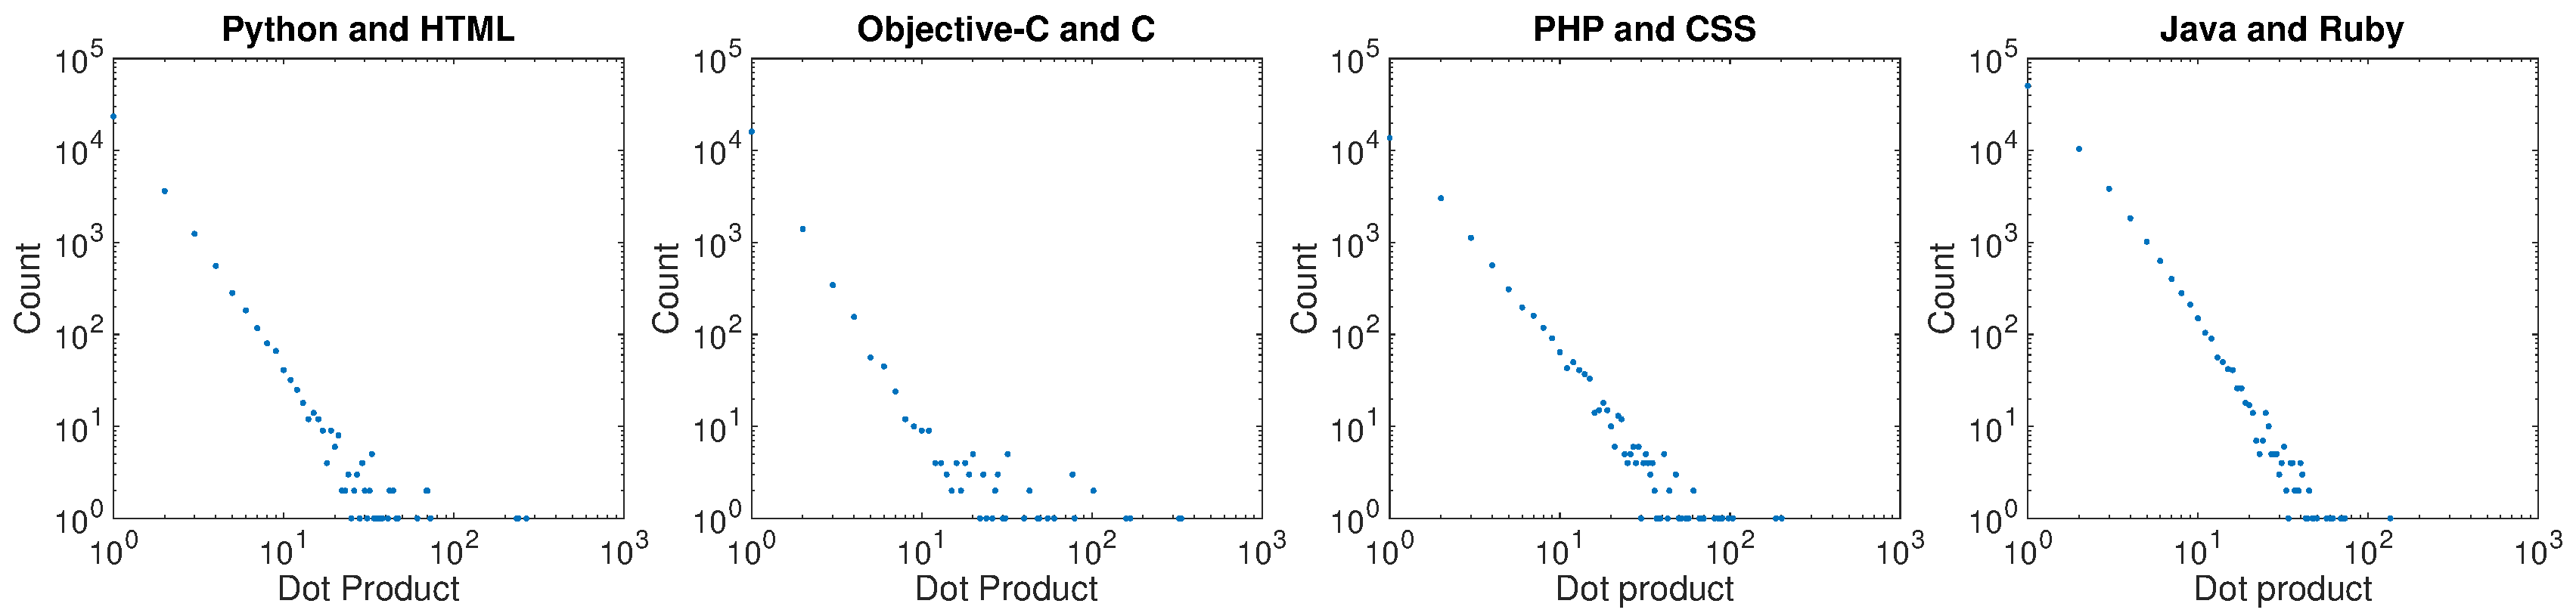
\includegraphics[width = 6 in]{figure/con_intersection_degree.eps}}
	\subcaptionbox{Cosine}{
		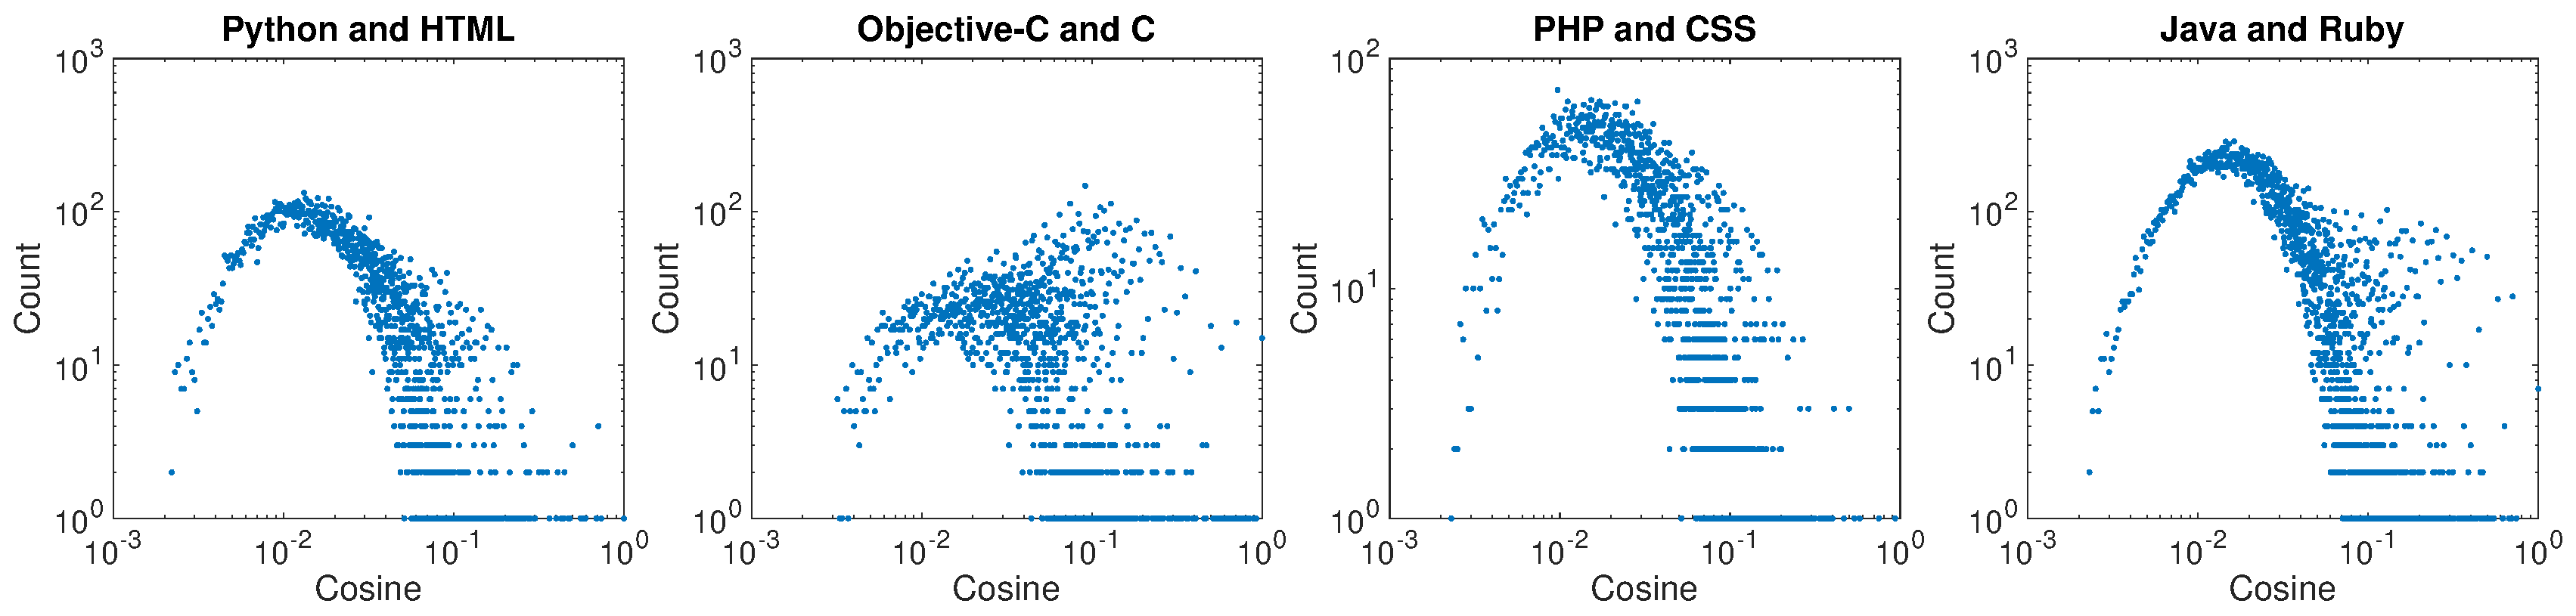
\includegraphics[width = 6 in]{figure/con_cosine_degree.eps}}
	\subcaptionbox{Jaccard}{
		\includegraphics[width = 6 in]{figure/con_Jaccard_degree.eps}}
	\subcaptionbox{Dot product + idf}{
		\includegraphics[width = 6 in]{figure/con_idf_intersection_degree.eps}}
	\subcaptionbox{Cosine + idf}{
		\includegraphics[width = 6 in]{figure/con_idf_cosine_degree.eps}}
	\caption{Weighting schemes distribution of subnetworks transformed from repository-contributor subnetworks}
	\label{fig:weight degree distribution of repository-contributor}
\end{figure*}


\begin{figure*}
	\centering
	\subcaptionbox{Dot product}{
		\includegraphics[width = 6 in]{figure/star_intersection_degree.eps}}
	\subcaptionbox{Cosine}{
		\includegraphics[width = 6 in]{figure/star_cosine_degree.eps}}
	\subcaptionbox{Jaccard}{
		\includegraphics[width = 6 in]{figure/star_Jaccard_degree.eps}}
	\subcaptionbox{Dot product + idf}{
		\includegraphics[width = 6 in]{figure/star_idf_intersection_degree.eps}}
	\subcaptionbox{Cosine + idf}{
		\includegraphics[width = 6 in]{figure/star_idf_cosine_degree.eps}}
	\caption{Weighting schemes distribution of subnetworks transformed from repository-stargazer subnetworks}
	\label{fig:weight degree distribution of repository-stargazer}
\end{figure*}

\subsection{Visualization of Clustering Results}
To find out the reason of the incorrect clustering, we labeled those repositories, which are clustered into the wrong communities, on the distribution of repositories. Because the clustering result of the repository network transformed from the repository-contributor is not good, we just plot those repository network obtained from the repository-contributor network. Figure \ref {fig:repository distribution labeled by greedy algorithm clustering results of repository-stargazer network} and Figure \ref{fig:repository distribution labeled by spectral algorithm clustering results of repository-stargazer network} separately display the clustering result of greedy modularity maximization optimization algorithm and spectral modularity optimization algorithm on all subnetworks transformed by different weighting schemes. In these figures, each colour represents a kind of repositories of the original label. The point means the repository is clustered into the correct community and the cross means the repository is clustered into the wrong community. We noticed that except those repositories are distributed into the other community are clustered incorrectly, most of the repositories clustered mistakenly is located on the border of two communities. In addition, we can clearly found that before applying the process of inverse document frequency, when we using dot product to transform the network, there are fewer repositories are clustered into the wrong communities. We also found that the inverse document frequency also decreases the rate of incorrect clustering, which is just as we have shown in \ref{fig:clustering result by greedy algorithm of repository-stargazer network} and Figure \ref{fig:clustering result by spectral algorithm of repository-stargazer network}. Then we separately selected a repository, which is incorrectly clustered for all the five different weighting scheme subnetworks, from four datasets and the detail of the repositories are shown in Table \ref{tab:example of repositories that are clustered into the wrong communities}. We can see that all of these repositories are written by at least three different programming languages and both of the languages we selected to labeled the dataset are included these programming languages. And these two languages are usually widely used in these repositories. So the composite application of programming languages may be the main reason cause the incorrect clustering.
\begin{figure*}
	\centering
	\subcaptionbox{Dot product}{
		\includegraphics[width = 6 in]{figure/star_intersection_greedy_wrong.eps}}
	\subcaptionbox{Cosine}{
		\includegraphics[width = 6 in]{figure/star_cosine_greedy_wrong.eps}}
	\subcaptionbox{Jaccard}{
		\includegraphics[width = 6 in]{figure/star_Jaccard_greedy_wrong.eps}}
	\subcaptionbox{Dot product + idf}{
		\includegraphics[width = 6 in]{figure/star_idf_intersection_greedy_wrong.eps}}
	\subcaptionbox{Cosine + idf}{
		\includegraphics[width = 6 in]{figure/star_idf_cosine_greedy_wrong.eps}}
	\caption{ Repository distribution labeled by greedy algorithm clustering results of subnetworks transformed from repository-stargazer subnetworks, point means repository is clustered into correct communities and cross means repository is clustered into wrong communities}
	\label{fig:repository distribution labeled by greedy algorithm clustering results of repository-stargazer network}
\end{figure*}

\begin{figure*}
	\centering
	\subcaptionbox{Dot product}{
		\includegraphics[width = 6 in]{figure/star_intersection_spectral_wrong.eps}}
	\subcaptionbox{Cosine}{
		\includegraphics[width = 6 in]{figure/star_cosine_spectral_wrong.eps}}
	\subcaptionbox{Jaccard}{
		\includegraphics[width = 6 in]{figure/star_Jaccard_spectral_wrong.eps}}
	\subcaptionbox{Dot product + idf}{
		\includegraphics[width = 6 in]{figure/star_idf_intersection_spectral_wrong.eps}}
	\subcaptionbox{Cosine + idf}{
		\includegraphics[width = 6 in]{figure/star_idf_cosine_spectral_wrong.eps}}
	\caption{Repository distribution labeled by spectral algorithm clustering results of subnetworks transformed from repository-stargazer subnetworks, point means repository is clustered into correct communities and cross means repository is clustered into wrong communities}
	\label{fig:repository distribution labeled by spectral algorithm clustering results of repository-stargazer network}
\end{figure*}

\begin{table*}
	\centering
	\begin{tabular}{c|ccc}  \toprule
		Repository ID & Dataset & Labeled Language & Actual Language \\ \hline
		\multirow{3}*{9089664}  & \multirow{3}*{PHP and CSS} & \multirow{3}*{PHP} & PHP 273765 \\
		& & &JavaScript	235403 \\
		& & &CSS	145940 \\ \hline
		\multirow{7}*{33945}  & \multirow{7}*{Java and Ruby} & \multirow{7}*{Java} & Java	716739 \\
		& & &Ruby	611648 \\
		& & &C	189161 \\
		& & &HTML	96249 \\
		& & &Yacc	7381 \\
		& & &Shell	3964 \\
		& & &XSLT	1868 \\ \hline
		\multirow{4}*{11766695}  & \multirow{4}*{Objective-C and C} & \multirow{4}*{C} & C	1359072 \\
		& & &Objective-C	212092 \\
		& & &C++	98486 \\
		& & &Ruby	1514 \\ \hline
		\multirow{5}*{27534934}  & \multirow{5}*{Python and HTML} & \multirow{5}*{Python} & Python	779863 \\
		& & &HTML	62123\\
		& & &CSS	5766 \\
		& & &JavaScript	2447 \\
		& & &Makefile	399 \\ \hline
	\end{tabular}
	\caption{Example of repositories that are clustered into the wrong communities by two clustering algorithms for all weighting schemes}
	\label{tab:example of repositories that are clustered into the wrong communities}
\end{table*}
%-------------------------------------------------------------------------------------
\section{Summary}
This section discussed the heterogeneous-transformed homogeneous clustering method for the homogeneous network clustering. We selected three different categories weight, dot product, cosine similarity and Jaccard similarity to transform the heterogeneous network to a homogeneous one.Then we use modularity optimization algorithm cluster the homogeneous network and evaluated the result by F-measure and rand index. Table \ref{tab:weighting schemes of best result} lists the weighting schemes when we get the best results on different datasets for both algorithms, and we found that for the repository-stargazer network, the combination of dot product and inverse document frequency perform better than other weight schemes for both clustering algorithms.  As the sparsity of repository-contributory, the clustering result is not satisfied. But we also found that we usually get the same clustering result of the greedy modularity maximization optimization algorithm, no matter which weighting schemes we select or whether apply the inverse document frequency. However, if we cluster the homogeneous by the spectral algorithm, the combination of cosine similarity and inverse document is the best choice. Therefore, for GitHub dataset, repository-stargazer network provides more information and dot product-idf is the best weighting schemes to describe the relation between repositories. 
%But for the different network, the best weighting scheme is different and different clustering algorithm also affect the choice of weighting schemes. And the inverse document frequency will improve the performance in general. In addition, we also found that the composite application of programming languages may cause incorrect clustering in our experiments.

\begin{table*}
\centering
\begin{tabular}{c|cc|cc} \toprule
\multirow{2}{*}{Dataset} & \multicolumn{2}{c}{Contributor} &  \multicolumn{2}{|c}{Stargazer} \\ \cline{2-5}
&Greedy & Spectral & Greedy & Spectral  \\ \hline
\multirow{5}{*}{}  
Python and HTML& all &  C + idf & D+idf & D +idf  \\
Objective-C and C & all & C+idf  & D+idf  & D+idf\\
PHP and CSS & all & C+idf & D & D+idf \\
Java and Ruby & all & C& D+idf & D+idf \\
\bottomrule
\end{tabular}
\caption{Weighting schemes for best result}
\label{tab:weighting schemes of best result}
\end{table*}
%-------------------------------------------------------------------------------------
\chapter{Communities in Repositories}\label{chapter:communities in repositories}
In previous sections, we have found that dot product-idf is the best weighting scheme to describe the relations between repositories. This section uses this weighting scheme to reveal the overall relationship between repositories and their communities.   

\section{Visualization of the Original Clusters}
Based on the whole repository-stargazer network that has been collected, we first transform the heterogeneous network to homogeneous repository network using dot product-idf and each repository can be represented as a vector, whose element is the distance from this repository to the others. This vector is further reduced to two dimensions using LargeVis .  All the repositories are plotted in fig \ref{fig:Original communities visualization}(a). In this figure, repositories with popular languages(at least has over 100 repositories) are labeled by different colours, and the rest of repositories are belong to otherwise. To clearly observe the relationship between different communities, we subplot some figures only including a few number of programming languages repositories. The result is shown in Figure \ref{fig:Original communities visualization}. From Figure  \ref{fig:Original communities visualization}(b), we can see that the distance between JavaScript with PHP is close and the repository of JavaScript, HTML and CSS and mixed together. Then we removed JavaScript repositories(Figure  \ref{fig:Original communities visualization}(c)), we found that the distance between HTML and CSS repository are tight, which means these two kinds of programming languages are usually used together.  Then we plot the JavaScript and Java repositories(Figure  \ref{fig:Original communities visualization}(d)), and we can clearly observe that these two categories of repositories are distributed into different areas and there is just a few repositories are close to the other kind of repositories. In Figure  \ref{fig:Original communities visualization}(e), we can see that the communities of Python, C, Go, and C++ are close to each other. While the repositories of C\# are distributed in the same area, which is far away from the communities of the other four programming languages. At last, we plot the repositories with Objective-C, Ruby, and Swift. From Figure  \ref{fig:Original communities visualization}(f), it is clearly shown that Objective-C is close to Swift, and both languages are used for OS X and iOS operating systems. However, the communities of Ruby are located away from these communities in the contrary direction.  
\begin{figure*}
	\centering
	\subcaptionbox{Whole network visualization}{
		\includegraphics[width = 2.5 in]{figure/All_plot.eps}}
	\subcaptionbox{JavaScript, PHP, HTML, CSS}{
		\includegraphics[width = 2.5 in]{figure/All_plot1.eps}}
	\subcaptionbox{PHP, HTML, CSS}{
		\includegraphics[width = 2.5 in]{figure/All_plot5.eps}}
	\subcaptionbox{JavaScript, Java}{
		\includegraphics[width = 2.5 in]{figure/All_plot4.eps}}
	\subcaptionbox{Python, C, Go, C++, C\#}{
		\includegraphics[width = 2.5 in]{figure/All_plot2.eps}}
	\subcaptionbox{Objective-C, Ruby, Swift}{
		\includegraphics[width = 2.5 in]{figure/All_plot3.eps}}
	\caption{Original communities visualization}
	\label{fig:Original communities visualization}
\end{figure*}
 
\section{Clustering Results}
Then we applied greedy modularity optimization algorithm and spectral modularity optimization algorithm on the repository network. Figure \ref{fig:Clustering results visualization} separately show the clustering results of these two algorithms. For greedy modularity optimization algorithm(Figure \ref{fig:Clustering results visualization}(a)), when we detect 7 communities, we get the highest modularity, 0.3050. At the same time, the value of F-measure and rand index is 0.4888 and 0.7932, respectively. Comparing with the original clusters, we can see that  Ruby repositories belong to community 1. Community 2 includes Python, C, C++, and Go repositories and in reality, people who like to use C also prefer to utilize C++, Python, and Go. Objective-C and Swift form communities 3 and both programming languages are designed by Apple Inc. Community 4 is mainly composed by repositories from JavaScript, HTML, PHP, and CSS. All of these programming languages are used for web developing. Java and C\# separately constitute community 5 and 6. Community 7 only includes 21 repositories, including 8 ActionScript repositories, 4 Haxe repositories,4 JavaScript repositories, 2 C++ repositories, 2 Shell repositories and 1 Dare repository. 

Figure \ref{fig:Clustering results visualization}(b) show the clustering result of spectral modularity optimization algorithm. From the figure we can see there are totally four communities. At this time, the value of modularity, F-measure and rand index are separately 0.253, 0.3287and 0.7009. All of these value are lower than the result of greedy algorithm, which means the result of greedy algorithm is closer to the ground truth. The four communities we have detected separately includes 4497, 2743, 398
and 3027 repositories. Unlike the greedy algorithm, the spectral algorithm merges Ruby repositories into the community 1 of JavaScript, HTML, PHP, and CSS. Java, Objective-C, and Swift compose community 2. Community 3 is located between Community 1 and 2, and most of the repositories of this community are JavaScript repository. Community 4 is mainly made up of Python, C, C++ and Go repositories. 

Comparing the results, we found the spectral algorithm detect fewer communities than greedy algorithm. Both clustering results present the relationship between communities of repositories. Each community is constructed by a serious of repositories with different programming languages. We can found that the programming languages belong to the same community are usually used together in practice. For instance, HTML, PHP, and CSS are used together to create web pages and web applications. Therefore, the clustering result shows the real reaction between programming languages in some degree. 

\begin{figure*}
	\centering
	\subcaptionbox{Greedy}{
		\includegraphics[width = 2.5 in]{figure/All_greedy.eps}}
	\subcaptionbox{Spectral}{
		\includegraphics[width = 2.5 in]{figure/All_spectral.eps}}
	\caption{Clustering results visualization}
	\label{fig:Clustering results visualization}
\end{figure*}
 
\chapter{Relationship between Programming Languages}\label{chapter:relationship between programming languages}
In this chapter, we investigate the relation between programming languages. We use three methods to cluster programming languages. One is based on the interaction between presuming languages and repositories and another is based on the relation between programming languages and users. In addition, we also reduced the matrix of programming languages-repositories to 2 dimensions and then detect the communities of programming languages. 
\section{Clustering using repositories}\label{subsection:Clustering using repositories}
Now we can study the relationship between programming languages based on repository interactions.  First, we need to find a vector representation for each language. We define the vector representation of language $L$ is the sum of all the vectors of the repositories in language $L$, i.e., 
\begin{align}
L=\sum_{R_i\in L} R_i, 
\end{align}
where $R_i$ is the vector representation of the $i$-th repository that is discussed in the last section. For example, Table \ref{tab:Repository-repository-matrix transform to Language-repository Matrix}(a) show a repository-repository matrix. Suppose repository R1, R2 are labeled by language L1, and R3, R4 belong to L2. Then we separately add the first , the second row, and the third, the fourth row together. We get the language-repository matrix and each language is represented as a vector. Based on the result of the last section, the most promising representations are dot product-idf. Hence, in the following discussions, we will focus on the weighting scheme only. 

\begin{table*}
	\subcaptionbox{Repository-repository matrix}{
		\begin{minipage}[b]{0.5\textwidth}
			\begin{center}
				\resizebox{2.5in}{0.52in}{
				\begin{tabular}{c|cccc} \toprule
					& R1 & R2 & R3 & R4 \\ \hline
					R1 & 0 & 5/16 & 1/16 & 5/16 \\
					R2 & 5/16 & 0 & 9/16 & 1/16 \\ 
					R3 & 1/16 & 9/16 & 0 & 5/16 \\ 
					R4 & 5/16 & 1/16 & 5/16 & 0 \\ \bottomrule
				\end{tabular}}
			\end{center}
		\end{minipage}}	
	\subcaptionbox{Language-repository matrix}{
		\begin{minipage}[b]{0.5\textwidth}
			\begin{center}
				\begin{tabular}{c|cccc} \toprule
					& R1 & R2 & R3 & R4 \\ \hline
					L1 & 5/16 & 5/16 & 10/16 & 6/16 \\ 
					L2 & 6/16 & 10/16 & 5/16 & 5/16 \\ \bottomrule
				\end{tabular}
			\end{center}
		\end{minipage}}	
	\caption{Repository-repository-matrix transform toLanguage-repository Matrix}
	\label{tab:Repository-repository-matrix transform to Language-repository Matrix}
\end{table*}

Once the language vectors are available, we can calculate their pairwise distances. We use cosine distance for the vectors. To reveal the hierarchical structure of programming languages, we apply HAC (hierarchical agglomerative clustering).

When running the HAC algorithms, the choice of the distance function for clusters is important. We tried several cluster distance functions, including single, complete, average, and weighted.  Single calculates the shortest distance between two clusters. On the contrary, complete calculate the furthest distance. Average represents the unweighted average distance and weighted means the inner squared distance. 

Figure \ref{fig:Dendrogram Tree for different linkage} show the dendrograms generated from various distance functions. From the plots, we can see that mostly the clustering results are similar, but weighted is slightly better than the others. In the following, we discussed the details of the clustering result using weighted as cluster distance function.
\begin{figure*}
	\centering
	\subcaptionbox{single}{
		\includegraphics[width = 3.5 in]{figure/lan_dendrogram_dot_cosine_single.eps}}
	\subcaptionbox{complete}{
		\includegraphics[width = 3.5 in]{figure/lan_dendrogram_dot_cosine_complete.eps}}
	\subcaptionbox{average}{
		\includegraphics[width = 3.5 in]{figure/lan_dendrogram_dot_cosine_average.eps}}
	\subcaptionbox{weighted}{
		\includegraphics[width = 3.5 in]{figure/lan_dendrogram_dot_cosine_weighted.eps}}
	\caption{Dendrogram Tree for different linkage}
	\label{fig:Dendrogram Tree for different linkage}
\end{figure*}

From the dendrogram (Figure \ref {fig:Dendrogram Tree of All Programming Languages}) and the heatmap (Figure \ref{fig:Spyplot of All Programming Languages})  we can observe that
\begin{itemize}
\item  For the dendrogram tree of dot product-idf(Figure\ref {fig:Dendrogram Tree of All Programming Languages}), there are mainly three clusters. The first one is from HTML to Puppet. In this cluster, HTML, CSS, JavaScript, and PHP are usually applied for web development. While Python, C, C++, and Go are used for system programming languages and python could also be used for web developing. Another community is the functional programming languages. From Scala to Red is the second clusters. In this cluster, most of the programming languages are not popular. And the rest programming languages constitute the last communities. This cluster includes Objective-C, Swift, and Objective-C++, which are designed by Apple Inc. for OS X and iOS operating system. And Java is also in this clusters with some other program languages, which is applied with Java or on the platform developed by Java, such as IDL and Groovy. 
%On the other hand, in Figure \ref {fig:Dendrogram Tree of All Programming Languages}(b), the merge order of programming languages is different and we can not clearly see the clusters.
\item Based on the order of the dendrogram tree, we separately draw the heatmap for both clustering schemes. In Figure \ref{fig:Spyplot of All Programming Languages}, we can see the distance between HTML, CSS and JavaScript are close and all these programming languages are usually used together for web developing. We also found python is popular language and connect with a lot of other languages. The connection between C and C++ is tight because C++ is generated from C. Java is close to IDL , which is used to describe interface written by Java, and Groovy, an object-oriented programming language for Java platform. Besides, Objective-C, Swift, and Objective-C++ connect tightly with each other as all of them designed by the same company, Apple. 
%Unlike the result of the dendrogram tree, in Figure \ref{fig:Spyplot of All Programming Languages}(b), we see the scene, although the order of programming languages is different. 
\end{itemize}

%\begin{figure*}
%	\centering
%	\subcaptionbox{Dendrogram}{
%		\includegraphics[width = 6 in]{figure/lan_dendrogram_dot_cosine_ward.eps}}
%	\vspace{3mm}	
%	\subcaptionbox{Heatmap}{
%			\includegraphics[width = 4.5 in]{figure/dot_lan_spyplot_cos_ward.eps}}
%	\caption{Clustering result using Intersection/idf as repository distance and WARD as cluster distance.}
%	\label{fig:Dendrogram Tree of All Programming Languages}
%\end{figure*}
%
%\begin{figure*}
%	\centering
%	\subcaptionbox{Dendrogram}{
%		\includegraphics[width = 6 in]{figure/lan_dendrogram_cos_cosine_ward.eps}}
%	\subcaptionbox{Heatmap}{
%		\includegraphics[width = 4.5 in]{figure/cosine_lan_spyplot_cos_ward.eps}}
%	\caption{Clustering result using cosine/idf as repository distance and WARD as cluster distance.}
%	\label{fig:Spyplot of All Programming Languages}
%\end{figure*}

\begin{figure*}
	\centering
	%\subcaptionbox{Dot Product-idf}{
		\includegraphics[width = 6 in,  height = 8.5in]{figure/lan_dendrogram_dot_cosine_weighted_left.eps}
		%}
	%\subcaptionbox{Cosine similarity-idf}{
	%	\includegraphics[width = 6 in]{figure/lan_dendrogram_cos_cosine_weighted.eps}}
	\caption{Dendrogram tree of all programming languages using cosine as repository distance and weighted as cluster distance}
	\label{fig:Dendrogram Tree of All Programming Languages}
\end{figure*}

\begin{figure*}
	\centering
	%\subcaptionbox{Dot Product-idf}{
		\includegraphics[width = 6.5 in]{figure/dot_lan_spyplot_cos_weighted.eps}
		%}
	%\subcaptionbox{Cosine similarity-idf}{
	%	\includegraphics[width = 4.5 in]{figure/cosine_lan_spyplot_cos_weighted.eps}}
	\caption{Heatmap of all programming languages using dot product-idf as repository distance and weighted as cluster distance}
	\label{fig:Spyplot of All Programming Languages}
\end{figure*}

\section{Clustering using users}\label{subsection:Clustering using users}
During the process of network transformation, we lost some information which may affect the relation between programming languages. To solve this problem, we directly qualify the relation based on the repository-stargazer network by mutual information(MI). Since each repository is labeled by one programming languages, we can transfer the repository-stargazer network to the language-stargazer matrix. If the user stars the repository labeled by the programming language, the value of the row of the programming language and the column of the user is 1, otherwise is 0. For example, Table \ref{tab:Repository-User matrix transform to Language-repository matrix}(a) show a repository-user matrix. Suppose repository R1, R2 are labeled by language L1, and R3, R4 belong to L2. We can see that both R1 and R2 are not connected with U6, so in Table \ref{tab:Repository-User matrix transform to Language-repository matrix}(b), for L1, the value of column U6 is 0. 
\begin{table*}
	\centering
	\subcaptionbox{Repository-user matrix}{
		\resizebox{2.5in}{0.52in}{
		\begin{tabular}{c|ccccccc} \toprule
			& U1 & U2 & U3 & U4 & U5 & U6 & U7\\ \hline
			R1 & 1 & 0 & 1 & 0& 0& 0& 1\\  
			R2 & 1 & 1 & 0 & 1& 1& 0& 1\\ 
			R3 & 0 & 1 & 0 & 1& 0& 1& 1\\ 
			R4 & 0 & 0 & 1 & 0& 0& 1& 1\\ \bottomrule
		\end{tabular}}
	}
	\subcaptionbox{Language-user matrix}{
		
		\begin{tabular}{c|ccccccc} \toprule
			& U1 & U2 & U3 & U4 & U5 & U6 & U7\\ \hline
			L1 & 1 & 1 & 1 & 1& 1& 0& 1\\  
			L2 & 0 & 1 & 1 & 1& 0& 1& 1\\ \bottomrule
		\end{tabular}
		}
	\caption{Repository-User matrix transform to Language-repository matrix}
	\label{tab:Repository-User matrix transform to Language-repository matrix}
\end{table*}

So We get the language-repository matrix and each language is represented as a vector. Then we can use the following mutual information to quantify the connection between programming language a and b:

\begin{equation}
	MI(a,b) = \dfrac{\log \dfrac{P_{ab}}{P_{a}P_{b}}}{-\log P_{ab}}
\end{equation}

where the probabilities $P_{a}$ and $P_{ab}$ is defined as follows. Suppose  $n_{a}$ is the number of users connect with programming languages a and $n_{ab}$ is the common users between two programming languages a and b. N is the total number of users. Then   $P_{a}= n_{a} / N $ and $P_{ab}=n_{ab}/N $. We add $-\log P_{ab}$ to normalize the value so that this value is in the range of -1 to 1. The positive value means there are more common users between these two programming languages than we expect, and a negative means there are less.  As the large number of users, we removed those users whose degree is less than 3 from the network. So we calculate the mutual information of 95 programming languages on 592,259 users. 

Then we plot the dendrogram tree of programming languages using mutual information as similarity measurement and the result is shown in Figure \ref{fig:dendro_mi}. This figure reveals some close pairs that are not so obvious, such as Julia\&Fortran, Stan\&R, Swift\&ObjectiveC. Julia and Fortran are close because Julia supports the direct call of Fortran code. Stan is a statistic tool that is integrated with R.  Swift is a successor of  ObjectiveC. Elixir runs on Erlang virtual machine. Groovy interoperates with Java code and library, runs on Java Virtual Machine.  Most valid Java programs are also valid for Groovy. There are also some obvious clusters of programming languages. For instance, C is close to C++ and python . C++ is designed based on C and the implementation of Python is written by C.Besides, HTML, CSS, PHP, JavaScript is also close to each other and all of these programming languages are used to web developing. 

The pairwise mutual information is plotted in Figure \ref{fig:Mutual Information between  Programming Languages}. Programming languages are sorted using hierarchical agglomerative clustering by average linkage. From this figure, we found the same result that web programming languages, functional programming languages and system programming languages separately compose a community. 

\begin{figure*}
	\centering
	\includegraphics[width = 6 in, height = 8.5in]{figure/lan_dendrogram_MI.eps}
	\caption{Clustering result using MI as similarity measurement}
	\label{fig:dendro_mi}
\end{figure*}

\begin{figure*}
	\centering
	\includegraphics[width = 6.5 in]{figure/MI_test.eps}
	\caption{Mutual Information between  Programming Languages}
	\label{fig:Mutual Information between  Programming Languages}
\end{figure*}

\begin{itemize}
\item Functional programming: common-lisp, racket, scheme, frege, Wisp:
\item OSX: ObjectiveC, Swift, Groff %(text formatting for Unix system, written by C++)
, ObjectiveC++, SQLPL
%(extend the use of SQL for IBM DB2) 
\item System programming: C, C++, Go,Shell
%(command-line interpreter)
\item Web development programming: JavaScript, CSS, HTML, PHP, XML, CoffeeScript 
\end{itemize}

\section{Clustering using reduced dimensionality}

Clustering high dimensional data is may not be accurate-- high dimensions cause the distance large, and thereby the differences between pairs of entities be small. In subsections \ref{subsection:Clustering using repositories} and  \ref{subsection:Clustering using users} , the dimension is separately in the order of $10^4$ for repositories, and $10^6$ for users. %This can be demonstrated in Fig.., where most distances are large.  
One remedy to the problem is to reduce the dimensions. Common approaches to dimensional reduction is PCA (principal component analysis), and more recently, t-SNE \cite{maaten2008visualizing}. t-SNE (t-distributed stochastic neighbour embedding) is suitable for embedding high dimensional data to two or three dimensions. This is particularly good for us to visualize the relations between languages using scatter plot, so that we can plot similar languages by nearby points.  In the following, we use t-SNE to reduce the dimensions. 


Given the Language-Repository $m\times n$ matrix M, 
\[
\begin{bmatrix}
L_{1,1} & L_{1,2} & \dots &L_{1,n} \\
L_{2,1} & L_{2,2} & \dots &L_{2,n} \\
\dots \\
L_{m,1} & L_{m,2} & \dots &L_{m,n} \\
\end{bmatrix}
\]

where m=94 and n=10,065. Each row is a vector representation of the language that is obtained in subsection \ref{subsection:Clustering using repositories}. we run t-SNE to turn this matrix to a $m\times 2$ matrix as below, so that each language is represented by a two dimensional vector. 

\[
\begin{bmatrix}
T_{1,1} & T_{1,2} \\
T_{2,1} & T_{2,2} \\
\dots \\
T_{m,1} & T_{m,2}  \\
\end{bmatrix}
\]

t-SNE is downloaded from https://github.com/lvdmaaten/bhtsne. The command to run the program is python bhtsne.py -i input file -o outpace -p 5 -d 2 -t 1 -v. The parameters include perplexity, dimension, and threads.  One important parameter is perplexity and we tried perplexity = 5, which is the one commonly used. 

Once the 2-dimensional vector representations are available for the languages, we run HAC using the Euclidean distance as defined by
\begin{align}
d_{ij}=\sqrt{(T_{i,1}-T_{j,1})^2+ (T_{i,2}-T_{j,2})^2} 
\end{align}

We run HAC using this distance function and use average as cluster distance. the resulting dendrogram and heatmap are shown in Figures \ref{fig:Dendrogram Tree of All Programming Languages based on language-language relation} and \ref{fig:Heatmap of All Programming Languages based on language-language relation}. In addition to the dendrogram and the heatmap, we now can scatter-plot 2-dimensional embeddings of the languages in fig \ref{fig:scatter-plot  Tree of All Programming Languages based on language-language relation}. 
\begin{figure*}
	\centering
	%\subcaptionbox{Dot Product-idf}{
		\includegraphics[width = 6 in, height = 8.5in]{figure/lan_pid_dendrogram_dot_average.eps}
		%}
	%\subcaptionbox{Cosine similarity-idf}{
	%	\includegraphics[width = 6 in]{figure/lan_pid_dendrogram_cos_average.eps}}
	\caption{Languages clustered by Euclidian distance when dimensions are reduced to two using t-SNE}
	\label{fig:Dendrogram Tree of All Programming Languages based on language-language relation}
\end{figure*}

\begin{figure*}
	\centering
	%\subcaptionbox{Dot Product-idf}{
		\includegraphics[width = 6.5 in]{figure/dot_lan_pid_heatmap.eps}
		%}
	%\subcaptionbox{Cosine similarity-idf}{
	%	\includegraphics[width = 4 in]{figure/cos_lan_pid_heatmap.eps}}
	\caption{Heatmap of All Programming Languages based on language-language relation}
	\label{fig:Heatmap of All Programming Languages based on language-language relation}
\end{figure*}

From these plots we can make the following observations.

\begin{itemize}
\item   Overall clustering results are close to previous methods. We can see close pairs, such as  C\&C++, Objective-C\&Swift, HTML\& CSS 
\item Figure \ref{fig:scatter-plot  Tree of All Programming Languages based on language-language relation} reveals more clustering information. We see, in both figures,  som closely knit communities that are far away from any other languages, i.e., the group contains languages Matlab, R, Stan, Fortran, Julia.
\end{itemize}

\begin{figure*}
	\centering
	%\subcaptionbox{Dot Product-idf}{
		\includegraphics[width = 6.5 in]{figure/lan_relation_all_dot.eps}
		%}
	%\subcaptionbox{Cosine similarity-idf}{
	%	\includegraphics[width = 4 in]{figure/lan_relation_all_cos.eps}}
	\caption{Scatter plot of two dimensional vectors of programming languages generated by t-SNE. Repository-repository proximity matrix is generated using dot product-idf weight}
	\label{fig:scatter-plot  Tree of All Programming Languages based on language-language relation}
\end{figure*}

\section{Summary}
We studied relations between languages based on distance between repositories and user interactions. Through the experiment, we found some interesting results. For example, no matter which method we used, C\&C++, HTML\&CSS, and Objective-C\&Swift are always connected closely. An interesting phenomenon is FORTRAN, Matlab, Stan, and Julia are usually clustered in the same community. All of these programming languages are used for data analysis for statistical computing and numeric computation. For all the three different clustering method, we can see that most of the programming languages are clustered in the same communities but there is also some difference. For instance, only for clustering using repositories, Common-Lisp and Emacs-Lisp are close. While for the other two methods, these two programming languages are in different clusters.
%-------------------------------------------------------------------------------------
\chapter{Conclusion and Future Work}\label{chapter:conclusion}
%-------------------------------------------------------------------------------------
In this thesis, we crawled around 12 million users from GitHub. Based on the user information, we collected over 1 million followers of users, around 10,000 popular repositories with at least 500 stars and the contributors and stargazers of these repositories. Then we discussed the heterogeneous-transformed homogeneous clustering method for the homogeneous network clustering. We selected three different categories weight, dot product, cosine similarity and Jaccard similarity to transform the heterogeneous network to a homogeneous one. Then we use modularity optimization algorithm cluster the homogeneous network and evaluated the result by F-measure and rand index. Through the experiments on the subdatasets of GitHub, we found that for the repository-stargazer network provides more information than the repository-contributor network. On the repository-stargazer network, the combination of dot product and inverse document frequency performs better than other weight schemes for both clustering algorithms. Next, we used dot product-idf as the weighting scheme to reveal the relationship between communities of the whole network. We separately detected 7 communities for greedy modularity algorithm and 4 communities for spectral modularity algorithm. From the result of both clustering algorithm, we found that there are some programming languages are usually belong to the same community, such web development programming languages(JavaScript, HTML, CSS and PHP), system programming languages(Python, C, C++ and Go) and programming languages for OS X and iOS system(Objective-C and Swift). 

We also investigated the relation between programming languages on different clustering methods. One is based on the repository interaction. Transforming the repository-repository matrix to language-repository matrix, each programming languages could be represented as a vector. Then we calculated the cosine distance between each vector and applied HAC (hierarchical agglomerative clustering) to get the hierarchical structure of programming languages.  As the high dimensional of the language-repository matrix, the clustering result may not be accurate. Then we apply t-SNE to reduce the matrix to 2 dimensions and ran HAC using Euclidean distance as the input. Besides, due to the transformation may lose some information, we directly use the language-user relation to cluster the programming languages. This time, we utilized the mutual information as the distance function to evaluate the relation between programming languages. Form the experiment, it is difficult to decide which methods better performs the relation between programming languages, but we found some common phenomenon. Some pairs of programming languages are usually close, such as HTML\&CSS, C\&C++, and Matlab\&FORTRAN. Overall, we find that languages fall into five communities, i.e., web and  scripting languages (JavaScrip, HTML, CSS, etc.), system programming languages (C, C++, Python, etc.), OS X and IOS programming languages (Objective-C, Swift, Objective-C++, etc.), numerical and statistical languages (Matlab, FORTRAN, Julia and R), and functional programming (Lisp, Scheme, Racket, Haskell, etc.).

Future work will be addressed better understand the relation between programming languages and it can be summarized below: 
\begin{itemize}
\item Data: the data is not large enough, especially the number of projects. When more projects are collected, we expect to have more programming languages. In addition to more comprehensive GitHub data, other data sources, such as GoogleCode, StatckOverflow, could be included. 
\item  Language label: a project normally involves multiple languages. currently we use the top language to label the project.  For each project, GitHub provides the lines of code for each language. The top language is the language that has the largest line of code.  A more accurate analysis is needed for multi-labeled projects. 
\item Network embedding:  we used t-SNE to reduce the dimensions. There are other dimensionality reduction techniques, in particular, network embedding techniques such as node2vec. 
\item Utilize user network: users are not isolated. they form a network by following links. this info could be utilized in network embedding. 
\item Compare with co-occurrence data: a project can use multiple languages. Thus, relations between languages can be quantified by their co-occurrences in projects. Existing analyses on co-occurrence data including the mining of association rules.  This could be improved, and compared with the relation inferred from user interactions. 
\end{itemize} 

%For now, we just collected 10,000 repository and 95 programming languages. The data is not large enough, especially the number of projects. When more projects are collected, we expect to have more programming languages. Besides, a repository normally involves multiple languages. Currently, Github use the top language, the one has the largest line of code, to label the repository.  For each repository, GitHub provides the lines of code for each language.  A more accurate analysis is needed for multi-labeled projects.  For the dimensions reducing, we used t-SNE. There are other dimensionality reduction techniques, in particular, network embedding techniques such as node2vec. We expect to try more new approaches in the future. 
\addcontentsline{toc}{chapter}{References}
\bibliography{Thesis.bib}



%\newpage
%\begin{appendix}
%A short description of all programming languages we have collected and most of the information comes from Wikipedia.
%\begin{table}[h]
%\tiny
%\begin{tabular}{p{2cm}|p{12cm}}
%\toprule
%Language & Summary \\ \hline
%JavaScript &  web develop programming language \\	
%Objective-C++& simply source code mixed with Objective-C and C++ class\\  
%Java& application developing programming language \\
%Arduino&  integrated development environment (IDE), which is a cross-platform application written in the programming language Java \\  
%Objective-C& main programming languages for iOS and OS X operating system\\
%Nginx& web server written in C\\  
%Python& application and web programming language\\
%Matlab& data analysis \\  
%Ruby&popular in Ruby-on-Rails, which is a web framework  \\
%D& Multi-paradigm system programming. reengineering of C++.\\  
%PostScript& used as a page description language in the electronic publishing and desktop publishing\\  
%PHP &web pages \\
%Perl6 & a version of perl \\  
%C & system programming language\\
%Scheme& Functional programming  \\  
%HTML& web mark up language \\
%Batchfile& scripting language for Windows\\  
%Go&developed by Google \\
%F\#&Multi-paradigm, cross platform, supported by Microsoft. .Net implementation of OCaml. \\  
%CSS&web stylesheet \\
%Vala& an object-oriented programming language with a self-hosting compiler that generates C code and uses the GObject system\\  
%C++& system programming language\\
%Pascal& an imperative and procedural programming language \\  
%Swift& extension of ObectiveC \\
%XML& makeup language\\  
%Shell& a computer program designed to be run by the Unix shell, a command-line interpreter\\
%IDL&Interface Definition Language \\  
%C\#& extension of C++\\
%MoonScript& a dynamic scripting language that compiles into Lua\\  
%VimL&Vim script \\
%wisp&  a Lisp programming language \\  
%CoffeeScript& Extension to JavaScripts, learnt from Ruby \\
%Modelica&modelling language \\  
%Clojure& a dialect of Lisp. \\
%Yacc& compiler generation in C\\  
%Scala& Improve shortcomings of Java. compiled into Java bytecode. functional. \\
%NSIS& Nullsoft Scriptable Install System is a tool that allows programmers to create such installers for Windows\\  
%Emacs Lisp&a dialect of the Lisp programming language used by the GNU Emacs and XEmacs text editors\\
%PLpgSQL& a procedural programming language supported by the PostgreSQL ORDBMS\\  
%Perl& scripting language \\
%Racket& functional programming, extension of Scheme \\  
%Lua& lightweight multi-paradigm. written in C\\
%AGS Script& game making, all the interactivity in the game is handled using scripts\\  
%Haskell& a standardized, general-purpose purely functional programming language\\
%\bottomrule
%\end{tabular}
%\end{table}
%
%\end{appendix}
%
%
%
%\begin{table*}
%\tiny
%\begin{tabular}{p{2cm}|p{12cm}} 
%\toprule
%Language & Summary \\ \hline
%SQLPL&  Structured Query Language Procedural Language and was developed by IBM as a set of commands that extend the use of SQL in the IBM DB2 (DB2 UDB Version 7) database system\\  
%Erlang& ericsson Language. For telephone applications. Initially implemented in Prolog. \\
%Mirah& previously called Duby, Ruby-like language, subset of Ruby. Compiled to JVM. \\  
%TeX& text formatting \\
%Awk& a programming language designed for text processing and typically used as a data extraction and reporting tool\\  
%Rust& multi-paradigm, sponsored by Mozilla.\\
%GLSL& OpenGL Shading Language is one of several commonly used shading languages for real-time rendering \\  
%Makefile& much like a shell script with additional directions, which qualify make to focus on the required lines\\
%FORTRAN& for numeric computation and scientific computing \\  
%Jupyter Notebook&a web application that allows you to create and share documents that contain live code, equations, visualizations and explanatory text\\
%Mathematica&  language used in Mathematica, a symbolic mathematical computation program, sometimes called a computer algebra program, used in many scientific, engineering, mathematical, and computing fields\\  
%TypeScript& superset of JavaScript by Microsoft \\
%Nix& package manager using functional language \\  
%Groovy& scripting language for the Java platform. Compiled to JVM. \\
%PigLatin& a language for using Hadoop  \\  
%ActionScript& an object-oriented script programming language for HyperCard,  it is a superset of the syntax and semantics of the language more widely known as JavaScript\\
%Protocol Buffer&  a language-neutral, platform-neutral extensible mechanism for serializing structured data\\  
%R& data analyses  statistical computing and graphics supported by the R Foundation for Statistical Computing\\
%Vue& used in probeVue, tracing environment by IBM. \\  
%OCaml& functional programming \\
%Nimrod& designed to be "efficient, expressive, and elegant",supporting metaprogramming, functional, message passing, procedural, and object-oriented programming styles by providing several features such as compile time code generation, algebraic data types, an elegant foreign function interface (FFI) with C and compiling to JavaScript\\  
%Assembly& a low-level programming language for a computer, or other programmable device, in which there is a very strong correspondence between the language and the architecture's machine code instructions\\
%CMake& cross-platform free and open-source software for managing the build process of software using a compiler-independent method. It has minimal dependencies, requiring only a C++ compiler on its own build system\\  
%Elixir& a variant of Erlang.\\
%Crystal& a general-purpose, object-oriented programming language, developed as open source software with syntax inspired by Ruby\\  
%PowerShell& a task automation and configuration management framework from Microsoft, consisting of a command-line shell and associated scripting language built on the .NET Framework\\
%KiCad& a free software suite for electronic design automation\\  
%Groff& is the GNU replacement for the troff and nroff text formatters. It is an original implementation written primarily in C++ and is modeled after ditroff\\
%PureBasic& a commercially distributed procedural computer programming language and integrated development environment based on BASIC and developed by Fantaisie Software for Windows 32/64-bit, Linux 32/64-bit, and Mac OS X\\  
%Haxe&  an open source, high-level, cross-platform, multi-paradigm programming language and compiler that can produce applications and source code for many different platforms from a single code-base\\
%Arc& a dialect of the Lisp programming language\\  
%Kotlin& compiled to JVM and JavaScript\\
%Handlebars& a semantic web template system\\  
%Common Lisp&functional programming \\
%Red& was made to overcome the limitations of the programming language Rebol\\  
%LiveScript&Indirect descendant of CoffeeScript. Compiles to JavaScript. Functional. \\
%QML& a user interface markup language\\  
%Eagle& graphic layout editor \\
%Puppet& open source configuration management tool\\ 
%\bottomrule
%\end{tabular}\end{table*}

\vita{
\begin{table}[htbp]
\begin{tabular}{p{0.3\linewidth}p{0.65\linewidth}}
	NAME:           & Zhongpei Zhang                                                                                                                                                          \\
	PLACE OF BIRTH: & Harbin, Heilongjiang province, China                                                                                                                                    \\
	YEAR OF BIRTH:  & 1989                                                                                                                                                                    \\
	EDUCATION:      & Heilongjiang University, B.Eng., Computer Science and Technology, Harbin, China, 2012
\vskip1em
University of Windsor, M.Sc in Computer Science, Windsor, Ontario, 2016
\end{tabular}
\end{table}
}

\end{document}  
